%\documentclass[letterpaper,11pt,oneside,reqno]{amsart}

\documentclass{preprint}

%%%%%%%%%%%%%%%%%%%%%%%%%%%%%%%%%%%%%%%%
% Packages
%%%%%%%%%%%%%%%%%%%%%%%%%%%%%%%%%%%%%%%%

\usepackage[marginparwidth=2.4cm, marginparsep=1mm]{geometry}
\geometry{verbose,letterpaper,tmargin=1.2in,bmargin=1.2in,lmargin=1.5in,rmargin=1.5in}

\usepackage[full]{textcomp}
\usepackage[osf]{newtxtext}
\usepackage[title,titletoc]{appendix}

\usepackage{ifthen} 
\usepackage{hyperref}
\usepackage{breakurl}
\usepackage{amsmath}
\usepackage{amssymb}
\usepackage{mhequ}
\usepackage{mhenvs}
\usepackage{mhsymb}
\usepackage{mathrsfs}
\usepackage{microtype}
\usepackage{wasysym}
\usepackage{centernot}
\usepackage{booktabs}
\usepackage{tikz}
\usetikzlibrary{snakes}
\usepackage{colortbl}

\usepackage{hyperref}
\usepackage{amsmath}
\usepackage{amssymb}
\usepackage{mathrsfs}
\usepackage{mathtools}
\usepackage{bbm}
\usepackage{enumitem}
\usepackage{graphicx} 
\usepackage{marginnote}
\usepackage{tikz}
\usepackage{framed}
\usepackage{comment}
\usepackage{esint}
\usepackage{xcolor}
\usepackage{stmaryrd}
\usepackage{subfig}

\allowdisplaybreaks

%%%%%%%%%%%%%%%%%%%%%%%%%%%%%%%%%%%%%%%%
% Settings
%%%%%%%%%%%%%%%%%%%%%%%%%%%%%%%%%%%%%%%%

\definecolor{darkblue}{rgb}{0.13,0.13,0.39}
%\hypersetup{colorlinks=true,urlcolor=darkblue,citecolor=darkblue,linkcolor=darkblue, pdftitle=MartingaleSPDEs, pdfauthor={P. Grazieschi}}
%\allowdisplaybreaks

%\numberwithin{equation}{section}
%\numberwithin{table}{section}

%%%%%%%%%%%%%%%%%%%%%%%%%%%%%%%%%%%%%%%%%
%% Bibliography
%%%%%%%%%%%%%%%%%%%%%%%%%%%%%%%%%%%%%%%%%
%
%\usepackage[style=alphabetic,sorting=nty,natbib=true,maxnames=99,isbn=false,doi=false,url=false,firstinits=true,hyperref=auto,arxiv=abs,backend=bibtex]{biblatex}
%\addbibresource{bibliography.bib}
%\AtEveryBibitem{%
%  \clearlist{language}}
%\DeclareFieldFormat[article,inbook,incollection,inproceedings,patent,thesis,unpublished]{title}{#1\isdot}
%\renewbibmacro{in:}{%
%  \ifentrytype{article}{}{%
%    \printtext{\bibstring{in}\intitlepunct}}} \setlength{\biblabelsep}{6pt}
%\defbibheading{apa}[\refname]{\section*{#1}}
%\DeclareFieldFormat{sentencecase}{\MakeSentenceCase{#1}} \renewbibmacro*{title}{%
%  \ifthenelse{\iffieldundef{title}\AND\iffieldundef{subtitle}}{}
%  {\ifthenelse{\ifentrytype{article}\OR\ifentrytype{inbook}%
%      \OR\ifentrytype{incollection}\OR\ifentrytype{inproceedings}%
%      \OR\ifentrytype{inreference}} {\printtext[title]{%
%        \printfield[sentencecase]{title}%
%        \setunit{\subtitlepunct}%
%        \printfield[sentencecase]{subtitle}}}%
%    {\printtext[title]{%
%        \printfield[titlecase]{title}%
%        \setunit{\subtitlepunct}%
%        \printfield[titlecase]{subtitle}}}%
%    \newunit}%
%  \printfield{titleaddon}}
%
%\makeatletter
%\renewcommand{\email}[2][]{%
%  \ifx\emails\@empty\relax\else{\g@addto@macro\emails{,\space}}\fi%
%  \@ifnotempty{#1}{\g@addto@macro\emails{\textrm{(#1)}\space}}%
%  \g@addto@macro\emails{#2}%
%}
%\makeatother
%
%\makeatletter
%\newcommand\RedeclareMathOperator{%
%  \@ifstar{\def\rmo@s{m}\rmo@redeclare}{\def\rmo@s{o}\rmo@redeclare}%
%}
%% this is taken from \renew@command
%\newcommand\rmo@redeclare[2]{%
%  \begingroup \escapechar\m@ne\xdef\@gtempa{{\string#1}}\endgroup
%  \expandafter\@ifundefined\@gtempa
%     {\@latex@error{\noexpand#1undefined}\@ehc}%
%     \relax
%  \expandafter\rmo@declmathop\rmo@s{#1}{#2}}
%% This is just \@declmathop without \@ifdefinable
%\newcommand\rmo@declmathop[3]{%
%  \DeclareRobustCommand{#2}{\qopname\newmcodes@#1{#3}}%
%}
%\@onlypreamble\RedeclareMathOperator
%\makeatother

%%%%%%%%%%%%%%%%%%%%%%%%%%%%%%%%%%%%%%%%
% Definitions
%%%%%%%%%%%%%%%%%%%%%%%%%%%%%%%%%%%%%%%%

% For the Ising-Kac model
\newcommand{\epsEH}{\mathfrak{e}}
\newcommand{\fm}{\mathfrak{m}}
\newcommand{\fa}{\mathfrak{a}}
\renewcommand{\fM}{\mathfrak{M}}
\newcommand{\dheat}{(\partial_t-\Delta_\ga)}
\def\Heps{\mathcal{H}_{\mathfrak{e}}}
\colorlet{symbols}{black}

\newcommand*{\ldouble}{\{\mskip-6mu\{}
\newcommand*{\rdouble}{\}\mskip-6mu\}}
\newcommand*{\ldoublebig}{\bigl\{\mskip-10mu\bigl\{}
\newcommand*{\rdoublebig}{\bigr\}\mskip-10mu\bigr\}}

% Theorems
%\newtheorem{theorem}{Theorem}[section] 
%\newtheorem{lemma}[theorem]{Lemma}
\newtheorem{assumption}{Assumption}
%\newtheorem{proposition}[theorem]{Proposition} 
%\newtheorem{corollary}[theorem]{Corollary}
%\theoremstyle{definition} 
%\newtheorem{remark}[theorem]{Remark} 
%\newtheorem{definition}[theorem]{Definition} 
%\newtheorem{example}[theorem]{Example}
%\newtheorem{conjec}[theorem]{Conjecture} 
%\newcounter{assum}
%\renewcommand{\theassum}{H\arabic{assum}}
%\newtheorem*{notation}{Notation}
%\newcommand{\thmtitle}[1]{{\bf(#1)}}

% Other symbols
\newcommand*{\dd}{\mathop{}\!\mathrm{d}}
\newcommand{\set}[1]{\llbracket #1 \rrbracket}
\def\deltae{\Delta_{\eps}}
\def\symbol#1{\textcolor{symbols}{#1}}
\def\1{\mathbbm{{1}}}
\def\s{\mathfrak{s}}
\def\X{\symbol{X}}
\def\Wick#1{\,\colon\!\! \phantom{1} #1 \phantom{1} \!\colon}
\def\CCE{\mathbb{E}}
\def\CCV{\mathbb{V}}
\def\CCG{\mathbb{G}}
\def\CCT{\mathbb{T}}
\newcommand\STAR{\scalebox{0.3}{\tikz{\node[draw,fill=black,star,star point height=.7em,minimum size=1em]{};}}}
\def\i{\mathfrak{i}}
\def\CK{\mathcal{K}}
\def\CO{\mathcal{O}}
\def\CB{\mathcal{B}}
\def\CP{\mathcal{P}}
\def\CT{\mathcal{T}}
\def\CA{\mathcal{A}}
\def\CG{\mathcal{G}}
\def\CE{\mathcal{E}}
\def\CR{\mathcal{R}}
\def\L{\mathtt{L}}
\def\var{\mathtt{var}}
\def\nil{\mathtt{nil}}
\def\CN{\mathcal{N}}
\def\bz{\mathbf{z}}
\def\fr{\mathbf{r}}
\def\kone{\mathbf{k_1}}
\def\ktwo{\mathbf{k_2}}
\def\kthree{\mathbf{k_3}}
\def\kfour{\mathbf{k_4}}
\def\fC{\mathfrak{C}}
\def\Cd{\mathtt{C}}
\def\n{\mathbf{n}}
\def\bbz{{\bf \bar z}}
\def\SC{\mathscr{C}}
\def\SD{\mathscr{D}}
\def\SY{\mathscr{Y}}
\def\CL{\mathcal{L}}
\def\nablae{\nabla_{\!\!\eps}}

\renewcommand\emptyset{\varnothing}

\newcommand{\myoverline}[1]{\,\overline{\!{#1}}}
\newcommand{\myring}[1]{\,\mathring{\!{#1}}}
\newcommand{\ringF}{\mathring{F}}
\newcommand{\lineF}{\myoverline{F}}
\newcommand{\ringlineF}{\myring{\myoverline{F}}}
\newcommand{\ringG}{\mathring{G}}
\newcommand{\lineG}{\myoverline{G}}
\newcommand{\ringlineG}{\myring{\myoverline{G}}}

\def\v{\nu}
\def\w{\omega}
\def\u{\upsilon}
\def\Amin{{A^{\!-}}}

\def\cadlag{c\`{a}dl\`{a}g }
\def\Cadlag{C\`{a}dl\`{a}g }
\def\BDG{Burkholder-Davis-Gundy }
\def\CH{\mathcal{H}}
\def\BH{\overline{\mathcal{H}}}
\def\fn{\mathfrak{n}}
\def\CD{\mathcal{D}}
\def\CC{\mathcal{C}}
\def\CI{\mathcal{I}}
\def\fR{\mathfrak{R}}
\def\fK{\mathfrak{K}}
\def\PPi{\mathbf{\Pi}}

% Mathbb letters
% \newcommand{\C}{\mathbb{C}}
\newcommand{\D}{\mathbf{D}}
%\newcommand{\E}{\mathbb{E}}
\newcommand{\M}{\mathbb{M}}
\newcommand{\KK}{\mathscr{K}}
\newcommand{\RR}{\mathscr{R}}
%\newcommand{\C}{\mathbb{C}}
\newcommand{\nn}{\mathbbm{n}}
%\newcommand{\N}{\mathbb{N}}
%\renewcommand{\P}{{\mathbb P}}
%\newcommand{\Q}{{\mathbb Q}}
%\newcommand{\R}{\mathbb{R}}
\newcommand{\T}{\mathbb{T}}
%\newcommand{\Z}{\mathbb{Z}}

% Mathbf letters

\def\rrr{\mathbf{r}}
\def\zz{\mathbf{z}}
\def\xx{\mathbf{x}}
\def\yy{\mathbf{y}}

% Mathfrak (or mathsf) letters 
\newcommand{\ee}{\mathfrak{e}}
\newcommand{\rr}{\mathsf{r}}

% Caligraphic
\newcommand{\Aa}{\mathcal{A}}
\newcommand{\Bb}{\mathcal{B}}
\newcommand{\Cc}{\CC}
\newcommand{\Dd}{\CD}
\newcommand{\Ff}{\mathscr{F}}
\newcommand{\Mm}{\mathcal{M}}
\newcommand{\Nm}{\mathfrak{N}}
\newcommand{\Ss}{\mathcal{S}}
\newcommand{\Zz}{\mathcal{Z}}
\newcommand{\bM}{\mathbf{M}}
\newcommand{\bW}{\mathbf{W}}
\newcommand{\G}{\mathcal{G}}
\newcommand{\RG}{\mathcal{RG}}
%\newcommand{\CW}{\mathcal{W}}

\newcommand{\SK}{\mathscr{K}}
\newcommand{\SR}{\mathscr{R}}

\newcommand{\MM}{\mathscr{M}}
\newcommand{\GG}{\mathscr{G}}
\newcommand{\FF}{\mathscr{F}}
\newcommand{\Kk}{\mathscr{K}}

% Greek letters
\newcommand{\al}{\alpha}
\newcommand{\be}{\beta}
\newcommand{\ga}{\gamma}
\newcommand{\de}{\delta	}
%\newcommand{\eps}{\varepsilon}
\newcommand{\ka}{\kappa}
\newcommand{\la}{\lambda}
\newcommand{\om}{\omega}
\newcommand{\ph}{\phi}
\newcommand{\si}{\sigma}
\def\scal#1{\langle#1\rangle}

% Operators
\DeclareMathOperator{\dist}{dist}
%\DeclareMathOperator{\supp}{Supp}
\newcommand{\ls}{\lesssim}
\renewcommand{\subset}{\subseteq}
\def\un#1{\underline{#1}}

%convenient
\renewcommand{\d}{\mathrm{d}}
\newcommand{\Err}{\mathrm{Err}}
\newcommand{\Ext}{\mathsf{Ext}}
\newcommand{\id}{\mathfrak{1}}
\newcommand{\TV}{\mathrm{TV}}
\newcommand{\ov}{\overline}
\newcommand{\td}{\widetilde}
\newcommand{\mcl}{\mathcal}
\newcommand{\msf}{\mathsf}
\newcommand{\Ll}{\left}
\newcommand{\Rr}{\right}
\newcommand{\cc}{\mathbf{c}}
\newcommand{\F}{\mathscr{F}}
\newcommand{\dk}{\delta_k}
\renewcommand{\hat}{\widehat}
\newcommand{\htau}{\widehat{\tau}}
\newcommand{\hPsi}{\widehat{\Psi}}
\newcommand{\hP}{\widehat{P}}
\renewcommand{\phi}{\varphi}
 								
% Our most commonly used Besov space 
\newcommand{\Ca}{\Cc^{|\tau|}}

%Definitions Sec 2
\newcommand{\hg}{h_{\ga}} 								%Rescaled field
\newcommand{\kg}{\ka_\ga} 								% Interaction kernel
\newcommand{\Kg}{K_\ga} 								% Interaction kernel in macroscopic coordinates
\newcommand{\LN}{\Lambda_N} 							% discrete space microscopic coordinates
\newcommand{\Le}{\Lambda_\eps}		 					% discrete space macroscopic coordinates
\newcommand{\SN}{\Sigma_N} 							% Spin configurations
\newcommand{\Hg}{\mathscr{H}_{\ga}} 						% Hamiltonian
\newcommand{\lbg}{\lambda_{\ga}} 							% Gibbs measure
\newcommand{\Zbg}{\mathscr{Z}_{\ga}} 						% Partition function
\newcommand{\LgN}{\mathscr{L}_{\ga}} 						% Generator
\newcommand{\cg}{c_{\ga}}		 	 					% Jump rate microscopic coordinates
\newcommand{\Cg}{C_\ga} 								% Jump rate macroscopic coordinates
\newcommand{\mg}{m_\ga} 								% noise in microscopic coordinates
\newcommand{\Mg}{M_\ga}  								% noise in macroscopic coordinates
\newcommand{\Dg}{\Delta_\ga}		 					% Approximation to Laplace operator
\renewcommand{\ae}{\star_\eps} 							% Convolution on macroscopic discrete torus
\newcommand{\Eg}{E_\ga} 								% Error term appearing in the equation due to expansion of tanh
\newcommand{\Xg}{X_{\ga}}		  						% The rescaled field - our main object
\newcommand{\co}{c_{\ga,2}}  								% Constant close to 1, due to inaccuracy of $\eps =\ga^2$
\newcommand{\ct}{c_{\ga,1}}  								% Constant close to 1, due to approximation of integral not exactly =1
\newcommand{\Xng}{X_\ga^0} 							% Approximate initial condition
\newcommand{\Xn}{X^0} 							% Initial condition
\newcommand{\CGG}{\mathfrak{c}_{\ga}} 					% gamma - dependent renormalisation constant
\newcommand{\fc}{\mathfrak{c}} 					% gamma - dependent

%Definitions Sec 3
\newcommand{\Xe}{X_\eps}		 						% Solution to approximated PDE
\newcommand{\Ze}{Z_\eps} 								% Approximation to SHE
\newcommand{\Ce}{\mathfrak{c}_\eps} 						% Renormalisation constant
%\def\RR#1{R_{t}^{:{#1}:}} 									% continuous R
\def\ZZ#1{Z^{:{#1}:}} 										% continous Z
\newcommand{\tZ}{\widetilde{Z}} 							% processes with strange initial datum
\newcommand{\tZz}{ \widetilde{Z}^{\colon 2 \colon}} 			% and the second
\newcommand{\tZd}{ \widetilde{Z}^{\colon 3 \colon}} 			% and the third
\newcommand{\hRe}{\hat{R}_{\eps,t}}
\def\hRE#1{\hat{R}_{\eps,t}^{:{#1}:}}

\makeatletter
\newcommand*\bigcdot{\mathpalette\bigcdot@{.5}}
\newcommand*\bigcdot@[2]{\mathbin{\vcenter{\hbox{\scalebox{#2}{$\m@th#1\bullet$}}}}}
\makeatother

%%%%%%%%%%%%%%%%%%%%%%%%%%%%%%%%%%%%%%%%
% Tikz
%%%%%%%%%%%%%%%%%%%%%%%%%%%%%%%%%%%%%%%%

\usetikzlibrary{shapes}
\usetikzlibrary{shapes.misc}
\usetikzlibrary{shapes.symbols}
\usetikzlibrary{decorations}
\usetikzlibrary{decorations.markings}
\usetikzlibrary{decorations.pathreplacing}
\usetikzlibrary{calc,intersections,through,backgrounds}

\def\checkmark{\tikz\fill[scale=0.4](0,.35) -- (.25,0) -- (1,.7) -- (.25,.15) -- cycle;} 

\colorlet{testcolor}{green!60!black}

\def\drawx{\draw[-,solid] (-3pt,-3pt) -- (3pt,3pt);\draw[-,solid] (-3pt,3pt) -- (3pt,-3pt);}
\tikzset{
	root/.style={circle,fill=testcolor,inner sep=0pt, minimum size=2mm},
	dot/.style={circle,fill=black,inner sep=0pt, minimum size=1mm},
	small_dot/.style={circle,fill=black,inner sep=0pt, minimum size=0.9mm},
	var/.style={circle,fill=white,draw=black,inner sep=0pt, minimum size=2mm},
	var_blue/.style={circle,fill=blue!20,draw=blue,inner sep=0pt, minimum size=2mm},
	var_very_blue/.style={circle,fill=blue,draw=blue,inner sep=0pt, minimum size=2mm},
	var_red_square/.style={regular polygon,regular polygon sides=4, draw, fill=red!20, draw=red, inner sep=0pt, minimum size=2.5mm, shape border rotate=45},
	var_red_triangle/.style={regular polygon,regular polygon sides=3, draw, fill=red!20, draw=red, inner sep=0pt, minimum size=3mm, shape border rotate=180},
	var_red/.style={circle,fill=red!20,draw=red,inner sep=0pt, minimum size=2mm},
	circ/.style={circle,fill=white,draw=black,inner sep=0pt, minimum size=1.2mm},
	keps/.style= {semithick,shorten >=1pt,shorten <=1pt,->},%{semithick,densely dashed,shorten >=1pt,shorten <=1pt,->},
	dotred/.style={circle,fill=black!50,inner sep=0pt, minimum size=2mm},
	generic/.style={semithick,shorten >=1pt,shorten <=1pt},
	gepsilon/.style={semithick,shorten >=1pt,shorten <=1pt,densely dashed},
	rootlab/.style={font=\scriptsize, transform canvas={yshift=-0.23cm}},
	dist/.style={ultra thick,draw=testcolor,shorten >=1pt,shorten <=1pt},
	testfcn/.style={ultra thick,testcolor,shorten >=1pt,shorten <=1pt,<-},
	testfcnx/.style={ultra thick,testcolor,shorten >=1pt,shorten <=1pt,<-,
		postaction={decorate,decoration={markings,mark=at position 0.6 with {\drawx}}}},
	kprime/.style={semithick,shorten >=1pt,shorten <=1pt,dotted,->},
	kprimex/.style={semithick,shorten >=1pt,shorten <=1pt,densely dashed,->,
		postaction={decorate,decoration={markings,mark=at position 0.4 with {\drawx}}}},
	kernel/.style={semithick,shorten >=1pt,shorten <=1pt,->},
	multx/.style={shorten >=1pt,shorten <=1pt,
		postaction={decorate,decoration={markings,mark=at position 0.5 with {\drawx}}}},
	kernelx/.style={semithick,shorten >=1pt,shorten <=1pt,->,
		postaction={decorate,decoration={markings,mark=at position 0.4 with {\drawx}}}},
	kepsilon/.style={semithick,shorten >=1pt,shorten <=1pt,densely dashed,->},
	kernel1/.style={->,semithick,shorten >=1pt,shorten <=1pt,postaction={decorate,decoration={markings,mark=at position 0.45 with {\draw[-] (0,-0.1) -- (0,0.1);}}}},
	kernel2/.style={->,semithick,shorten >=1pt,shorten <=1pt,postaction={decorate,decoration={markings,mark=at position 0.45 with {\draw[-] (0.05,-0.1) -- (0.05,0.1);\draw[-] (-0.05,-0.1) -- (-0.05,0.1);}}}},
	kernelBig/.style={semithick,shorten >=1pt,shorten <=1pt,decorate, decoration={zigzag,amplitude=1.5pt,segment length = 3pt,pre length=2pt,post length=2pt}},
	rho/.style={dotted,semithick,shorten >=1pt,shorten <=1pt},
	renorm/.style={shape=circle,fill=white,inner sep=1pt},
	labl/.style={shape=rectangle,fill=white,inner sep=1pt},
	xi/.style={circle,fill=symbols!10,draw=symbols,inner sep=0pt,minimum size=1.2mm},
	xix/.style={crosscircle,fill=symbols!10,draw=symbols,inner sep=0pt,minimum size=1.2mm},
	xib/.style={circle,fill=symbols!10,draw=symbols,inner sep=0pt,minimum size=1.6mm},
	xibx/.style={crosscircle,fill=symbols!10,draw=symbols,inner sep=0pt,minimum size=1.6mm},
	not/.style={circle,fill=symbols,draw=symbols,inner sep=0pt,minimum size=0.5mm},
	>=stealth,
	}


\def\drawx{\draw[-,solid] (-3pt,-3pt) -- (3pt,3pt);\draw[-,solid] (-3pt,3pt) -- (3pt,-3pt);}
\tikzset{
	root/.style={circle,fill=testcolor,inner sep=0pt, minimum size=2mm},
	dot/.style={circle,fill=black,inner sep=0pt, minimum size=1mm},
	empty_dot/.style={circle, draw=black,fill=white,inner sep=0pt, minimum size=1mm},
	small_dot/.style={circle,fill=black,inner sep=0pt, minimum size=0.9mm},
	var/.style={circle,fill=white,draw=black,inner sep=0pt, minimum size=2mm},
	var_blue/.style={circle,fill=blue!20,draw=blue,inner sep=0pt, minimum size=2mm},
	var_very_blue/.style={circle,fill=blue,draw=blue,inner sep=0pt, minimum size=2mm},
	var_teal/.style={circle,fill=teal!20, draw=teal,inner sep=0pt, minimum size=2mm},
	var_red_square/.style={regular polygon,regular polygon sides=4, draw, fill=red!20, draw=red, inner sep=0pt, minimum size=2.5mm, shape border rotate=45},
	var_red_triangle/.style={regular polygon,regular polygon sides=3, draw, fill=red!20, draw=red, inner sep=0pt, minimum size=3mm, shape border rotate=180},
	var_red/.style={circle,fill=red!20,draw=red,inner sep=0pt, minimum size=2mm},
	circ/.style={circle,fill=white,draw=black,inner sep=0pt, minimum size=1.2mm},
	keps/.style= {semithick,shorten >=1pt,shorten <=1pt,->},%{semithick,densely dashed,shorten >=1pt,shorten <=1pt,->},
	keps-random/.style= {semithick,shorten >=1pt,shorten <=1pt,->, decorate, decoration = {zigzag, segment length=1mm, amplitude=1mm}},
	kepsdot/.style= {semithick,densely dashed,shorten >=1pt,shorten <=1pt,->},
	dotred/.style={circle,fill=black!50,inner sep=0pt, minimum size=2mm},
	generic/.style={semithick,shorten >=1pt,shorten <=1pt},
	gepsilon/.style={semithick,shorten >=1pt,shorten <=1pt,densely dashed},
	rootlab/.style={font=\scriptsize, transform canvas={yshift=-0.23cm}},
	dist/.style={ultra thick,draw=testcolor,shorten >=1pt,shorten <=1pt},
	testfcn/.style={ultra thick,testcolor,shorten >=1pt,shorten <=1pt,<-},
	testfcnx/.style={ultra thick,testcolor,shorten >=1pt,shorten <=1pt,<-,
		postaction={decorate,decoration={markings,mark=at position 0.6 with {\drawx}}}},
	kprime/.style={semithick,shorten >=1pt,shorten <=1pt,dotted,->},
	kprimex/.style={semithick,shorten >=1pt,shorten <=1pt,densely dashed,->,
		postaction={decorate,decoration={markings,mark=at position 0.4 with {\drawx}}}},
	kernel/.style={semithick,shorten >=1pt,shorten <=1pt,->},
	multx/.style={shorten >=1pt,shorten <=1pt,
		postaction={decorate,decoration={markings,mark=at position 0.5 with {\drawx}}}},
	kernelx/.style={semithick,shorten >=1pt,shorten <=1pt,->,
		postaction={decorate,decoration={markings,mark=at position 0.4 with {\drawx}}}},
	kepsilon/.style={semithick,shorten >=1pt,shorten <=1pt,densely dashed,->},
	kernel1/.style={->,semithick,shorten >=1pt,shorten <=1pt,postaction={decorate,decoration={markings,mark=at position 0.45 with {\draw[-] (0,-0.1) -- (0,0.1);}}}},
	kernel2/.style={->,semithick,shorten >=1pt,shorten <=1pt,postaction={decorate,decoration={markings,mark=at position 0.45 with {\draw[-] (0.05,-0.1) -- (0.05,0.1);\draw[-] (-0.05,-0.1) -- (-0.05,0.1);}}}},
	kernelBig/.style={semithick,shorten >=1pt,shorten <=1pt,decorate, decoration={zigzag,amplitude=1.5pt,segment length = 3pt,pre length=2pt,post length=2pt}},
	rho/.style={dotted,semithick,shorten >=1pt,shorten <=1pt},
	renorm/.style={shape=circle,fill=white,inner sep=1pt},
	labl/.style={shape=rectangle,fill=white,inner sep=1pt},
	xi/.style={circle,fill=symbols!10,draw=symbols,inner sep=0pt,minimum size=1.2mm},
	xix/.style={crosscircle,fill=symbols!10,draw=symbols,inner sep=0pt,minimum size=1.2mm},
	xib/.style={circle,fill=symbols!10,draw=symbols,inner sep=0pt,minimum size=1.6mm},
	xibx/.style={crosscircle,fill=symbols!10,draw=symbols,inner sep=0pt,minimum size=1.6mm},
	not/.style={circle,fill=symbols,draw=symbols,inner sep=0pt,minimum size=0.5mm},
	>=stealth,
	}
	

\makeatletter
\def\DeclareSymbol#1#2#3{\expandafter\gdef\csname MH@symb@#1\endcsname{\tikz[baseline=#2,scale=0.15,draw=symbols]{#3}}\expandafter\gdef\csname MH@symb@#1s\endcsname{\scalebox{0.7}{\tikz[baseline=#2,scale=0.15,draw=symbols]{#3}}}}
\def\<#1>{\csname MH@symb@#1\endcsname}
\makeatother

% Trees
\DeclareSymbol{1}{0}{\draw[white] (-.4,0) -- (.4,0); \draw (0,0)  -- (0,1.4) node[dot] {};}
\DeclareSymbol{2}{0}{\draw (-0.5,1.3) node[dot] {} -- (0,0) -- (0.5,1.3) node[dot] {};}
\DeclareSymbol{3}{0}{\draw (0,0) -- (0,1.3) node[dot] {}; \draw (-.7,1) node[dot] {} -- (0,0) -- (.7,1) node[dot] {};}
\DeclareSymbol{30}{-3}{\draw (0,0) -- (0,-1); \draw (0,0) -- (0,1.3) node[dot] {}; \draw (-.7,1) node[dot] {} -- (0,0) -- (.7,1) node[dot] {};}
\DeclareSymbol{31}{-3}{\draw (0,0) -- (0,-1) -- (1,0) node[dot] {}; \draw (0,0) -- (0,1.3) node[dot] {}; \draw (-.7,1) node[dot] {} -- (0,0) -- (.7,1) node[dot] {};}
\DeclareSymbol{32}{-3}{\draw (0,0) -- (0,-1) -- (1,0) node[dot] {}; \draw (0,0) -- (0,-1) -- (-1,0) node[dot] {}; \draw (0,0) -- (0,1.3) node[dot] {}; \draw (-.7,1) node[dot] {} -- (0,0) -- (.7,1) node[dot] {};}
\DeclareSymbol{20}{-3}{\draw (0,0) -- (0,-1);\draw (-.7,1) node[dot] {} -- (0,0) -- (.7,1) node[dot] {};}
\DeclareSymbol{22}{-3}{\draw (0,0.3) -- (0,-1) -- (1,0) node[dot] {}; \draw (0,0.3) -- (0,-1) -- (-1,0) node[dot] {};\draw (-.7,1) node[dot] {} -- (0,0.3) -- (.7,1) node[dot] {};}

% Contractions
\def\check{\tikz\fill[scale=0.4](0,.35) -- (.25,0) -- (1,.7) -- (.25,.15) -- cycle;} 

%%%%%%%%%%%%%%%%%%%%%%%%%%%%%%%%%%%%%%%%
% Comments
%%%%%%%%%%%%%%%%%%%%%%%%%%%%%%%%%%%%%%%%

\def\km#1{\marginnote{\color{teal}{\scriptsize{KM: #1}}}}
\def\kmtext#1{{\color{teal}{(KM: #1)}}}
\def\pg#1{\marginnote{\color{red}{\scriptsize{PG: #1}}}}
\def\pgtext#1{{\color{red}{PG: #1}}}
\def\hw#1{\marginnote{\color{testcolor}{\scriptsize{HW: #1}}}}
\def\hwtext#1{{\color{testcolor}{HW: #1}}}

\begin{document}

\date{\today}
\title{Martingale-driven integrals and singular SPDEs}
\author{P.~Grazieschi$^1$, K.~Matetski$^2$ and H.~Weber$^3$}
\institute{University of Bath, \email{p.grazieschi@bath.ac.uk} \and Michigan State University, \email{matetski@msu.edu} \and University of M\"{u}nster, \email{hendrik.weber@uni-muenster.de}}
\date{\today}
\titleindent=0.65cm

\maketitle

%\date{\today}
%\author[P.~Grazieschi]{Paolo Grazieschi}
%\author[K.~Matetski]{Konstantin Matetski}
%\author[H.~Weber]{Hendrik Weber}
%\address[P.~Grazieschi, H.~Weber]{Department of Mathematical Sciences, University of Bath, Bath, BA2~7AY, United Kingdom}
%\address[K.~Matetski]{Columbia University, Department of Mathematics, 2990 Broadway, New York, NY 10027, USA}
%\email[P.~Grazieschi]{p.grazieschi@bath.ac.uk}
%\email[K.~Matetski]{matetski@math.columbia.edu}
%\email[H.~Weber]{h.weber@bath.ac.uk}

\begin{abstract}
We consider multiple stochastic integrals with respect to \cadlag martingales, which approximate a cylindrical Wiener process. We define a chaos expansion, analogous to the case of multiple Wiener stochastic integrals, for these integrals and use it to show moment bounds. Key tools include an iteration of the \BDG inequality and a multi-scale decomposition similar to the one developed in \cite{HQ18}.
 Our method can be combined with the recently developed discretisation framework for regularity structures  \cite{HM18, EH19} to prove convergence of interacting particle systems to singular stochastic PDEs.  A companion article \cite{3dIsingKac} applies the results of this paper to prove convergence of a rescaled Glauber dynamics for the three-dimensional Ising-Kac model near criticality to the $\Phi^4_3$ dynamics on a torus.
\end{abstract}

\setcounter{tocdepth}{1}
\tableofcontents

\section{Introduction}

% 
% 
% \vskip2cm
% 
% **** 
% 
% End of sketch
% 
%*****
%
%\vskip2cm

%
%\newpage

We consider a class of \cadlag martingales which approximate a cylindrical Wiener process over a $d$-dimensional spatial domain, i.e. integrated-in-time space-time white noise. 
We develop a theory of iterated integrals with respect to these martingales and derive moment bounds. 


Our results serve as a technical tool for proving the convergence of Interacting Particle Systems (IPSs) to solutions of non-linear stochastic partial differential equations (SPDEs). The limiting SPDEs are usually of the form 
%
\begin{equation}\label{eq:general}
	\CL u = F(u,\nabla u) + \sigma(u) \xi,
\end{equation}
%
where $\CL$ is a linear parabolic operator (e.g. $\CL = \partial_t - \Delta$), $\xi$ is an irregular random noise (e.g. a Gaussian white noise) and $F$ and $\sigma$ are  local non-linearities. 
%
There are by now a number of convergence results of this type. These include $1+1$-dimensional surface growth models rescaling to the KPZ equation
%
\begin{equation}\label{eq:KPZ}
\partial_t  h - \partial_x^2 h = -  (\partial_x h)^2 + \xi,
\end{equation}
%
e.g. \cite{BG,MR3176353,Dembo:2013aa,1505.04158,1602.01908}, long range (Kac) spin models 
rescaling to $\phi^{2n}$ dynamics
%
\begin{equation}\label{eq:phi_2n}
\partial_t \phi - \Delta \phi = - \phi^{2n-1} + \xi,
\end{equation}
%
in one  \cite{MR1317994,FR} and two dimensions \cite{MR1661764,IsingKac,ShenWeber,Iberti}  as well as
diffusions in random environment rescaling to the parabolic Anderson model / multiplicative stochastic heat equation 
%
\begin{equation}\label{eq:SHE}
\partial_t u - \Delta u = u \xi, 
\end{equation}
\cite{MartinPerkowski,EH21}. Ultimately, the  motivating goal of the theory developed in this article is to show the convergence of the Ising-Kac model to the $\phi^4$ dynamics in three dimensions, and this is accomplished in our companion article \cite{3dIsingKac}. 

A common feature of all of these limiting results is that particle systems are simultaneously rescaled (i.e. observed on large scales) while a certain parameter is changed. The specific nature of this parameter depends on the model under consideration; examples are the strength of the \emph{weak} asymmetry in exclusion processes approximating the KPZ equation \cite{BG}, or the range of the interaction in Kac-models \cite{MR1661764}.  The typical strategy is to tune down the effect of the ``non-linearity'' as one moves to larger scales. 
%  E.g. WASEP or Kac-potential. 
This procedure is necessary to obtain convergence to one of the SPDEs \eqref{eq:KPZ}, \eqref{eq:phi_2n}, \eqref{eq:SHE}   and  reflects the fact that the SPDEs are themselves not scale-invariant. The fact that a relatively small class of SPDEs arises as scaling limit of this type for a relatively large number of particle systems sharing just a few key characteristics is sometimes referred to as  weak universality.

A key  technical challenge in deriving such scaling results is the low regularity of the solutions of the limiting equations \eqref{eq:KPZ},\eqref{eq:phi_2n},\eqref{eq:SHE}: the noise term $\xi$ is typically very irregular, leading to irregular solutions which in turn lead to difficulties in dealing with the non-linearities. This problem does not appear in more common Gaussian fluctuation limits \cite{KL99} --- while the solutions of the limiting equations there are typically also irregular, this is less problematic due to the absence of a non-linear term.
Good theories for non-linear SPDEs  and their renormalisation have only been developed over the last years, including Hairer's theory of regularity structures \cite{Regularity}, the theory of paracontrolled distributions put forward by Gubinelli, Imkeller and Perkowski \cite{MR3406823} and more recently theories of weak solutions for specific equations, in particular the KPZ equation \cite{MR3176353,MR3327509,MR3758149,MR4168394}.

The theory of regularity structures and the theory of paracontrolled distributions both build on a two-step approach: first, the construction of approximate solutions building a local expansion (the \emph{model} in the jargon of \cite{Regularity}) which relies on probabilistic tools, in particular Gaussian analysis and explicit calculations of covariance functions, and  second, analytic techniques (in particular regularity estimates and commutator estimates) for  dealing with the remainder. 
The weak solution theories developed in \cite{MR3176353,MR3327509,MR3758149,MR4168394} use a very different approach and make explicit use of the invariant Gaussian measure to give a direct characterisation of the generator of the dynamics. 

In principle, both approaches can be used to study scaling limits. In situations, where a simple invariant measure for an interacting particle system is given, the weak solution approach has proved highly efficient, see e.g.  \cite{MR3176353,MR4312852,MR4060852,MR3908648}. The approach which consists of mimicking the theory of regularity structure / paracontrolled distributions has also been implemented in a few examples, in particular \cite{IsingKac,MartinPerkowski,MR3592748,EH21}. 
%
Still,  implementing this programme for ``interesting'' limiting equations remains a challenging enterprise: for the second, deterministic, step of the analysis a systematic theory has been developed in \cite{HM18,EH19}, but the first probabilistic part remains challenging, because the number of terms in this perturbative expansion (the ``trees'') can become prohibitively large when looking at interesting equations. For the continuum there is by now a very systematic treatment for the trees (see \cite{HQ18,1612.08138,OttoTsatsoulisAlia,Hairer_Steele}). The aim of this paper is to develop a --- at least somewhat --- systematic approach to bound these trees for approximations of white noise. A particular focus is on the jump martingales that typically arise in the analysis of IPSs. 

On a technical level: the noise approximations we deal with are of bounded variation, but discontinuous because of the jumps. Therefore, the non-linear functionals that make up the model can rigorously be written in terms of integrals with respect to product measure in the underlying noise. We then decompose these integrals according to ``diagonals'' or ``contractions''. This is in the spirit of the Wiener chaos decomposition, however many more terms than in the Gaussian case arise, as in the latter only diagonals where precisely two coordinates coincide, make a non-vanishing contribution. In our noise approximations, many more ``diagonals'' appear and  we aim to show that their impact vanishes as space-time white noise is approached. 
Our main technical tool is an iteration of a \BDG (BDG) type inequality. For our purpose, the most convenient form is in terms of the predictable quadratic variation with an error term that depends on the size of jumps, as was used previously in \cite{IsingKac} . The advantage is that under our assumptions (which are motivated by the analysis of the Ising-Kac model \cite{3dIsingKac}), explicit and optimal bound on the predictable quadratic variation are available. The error term does not matter too much in the Ising-Kac application, because the size of individual jumps is suppressed by the smoothing from the Kac-potential.
Another key assumption we need to make, is that the magnitude of the jumps of the martingales is fixed by a deterministic constant. This allows to rewrite contractions of an odd number of variables in terms of a martingale and ultimately permits to prove that in the Kac-Ising application these contractions  vanish in the limit, even though they are integrated against a very singular kernel. 



\subsection{Structure of the article}

In Section~\ref{sec:MultIntegrals} we define multiple stochastic integrals with respect to \cadlag~square integrable martingales. In Section~\ref{sec:OneFoldBounds} we derive moment bounds on stochastic integrals with respect to only one variable, while moment bounds on multiple integrals are obtained in Section~\ref{sec:GeneralBounds}. Section~\ref{sec:renormalized-integrals} is devoted to renormalised stochastic integrals and their moment bounds. In Section~\ref{sec:GeneralizedConvolutions} we analyse stochastic integrals with kernels given by generalised convolutions, which are typical objects in the theory of regularity structures. As an example, we apply the result in Section~\ref{sec:applicationStochQuant} to a discrete approximation of the $\Phi^4_3$ equation. 
Some background material is collected in the two appendices.

\subsection{Notation}
We use the standard notation $\N = \{ 1, 2, 3, \ldots \}$ for the set of natural numbers, $\N_0$ for $\N \cup \{ 0 \}$ and the set $\R_+ := [0, \infty)$ for the time variables. For $n \in \N$ we define $\set{n} := \{ 1, \ldots, n \}$.\label{lab:set_n} We use $\1_A$ for the indicator function of the set $A$.

For $\Lambda_0$ being either $(\R / \Z)^d$ or $\R^d$ we use the standard notation $\SD'(\Lambda_0)$ for the space of distributions on $\Lambda_0$. For $n \geq 0$, the space $\SC^n(\Lambda_0)$ contains all $n$-times continuously differentiable functions on $\Lambda_0$, and we write $\SC(\Lambda_0)$ for this space when $n = 0$. The Skorokhod space of \cadlag functions on $[0, T]$ with values in $\SD'(\Lambda_0)$ is denoted by $D([0,T], \SD'(\Lambda_0))$. 

Given a random variable $X$ and some $p \geq 1$, we use the following shorthand notation for the $p^{\text{th}}$ moment 
\begin{equation}\label{eq:MomentNotation}
	\E_p X :=  \E \big[ | X |^p \big]^{1 / p}.
\end{equation}

In estimates we often use ``$\lesssim$'', which means that the bound ``$\leq$'' holds up to a constant which is independent of the quantities relevant in our statements, which will be always clear from the context. If we want to indicate dependence of the proportionality constant on some parameters $\alpha$, $\beta$, $\ldots$, we write ``$\lesssim_{\alpha, \beta, \ldots}$''.

For a bounded interval $I \subset \R$ with Lebesgue measure $|I| > 0$, we define the average of $f : \R \to \R$ over the interval $I$ as
\begin{equation}\label{eq:fintDef}
	\fint_{I} f(r) \d r := \frac{1}{|I|} \int_{I} f(r) \d r.
\end{equation}

Finally, let $\Le \subset \R^d$ be a lattice with mesh size $\eps$ (we will always consider $\Le$ to be either $(\eps \Z)^d$ or $(\eps \Z \slash \Z)^d$). For $T > 0$, $p \geq 1$ and for a function $F: [0, T] \times \Le \to \R$, we define
\begin{equation}\label{eq:norm-eps}
	\Vert F \Vert_{L^p_\eps} := \biggl( \eps^d \sum_{x \in \Le} \int_{0}^T | F(r,x) |^p \d r \biggr)^{\frac{1}{p}},
\end{equation}
that is, we take the $L^p$ norm in time and the $l^p$ norm in space with a weight $\eps^d$ on the points of the lattice. This and several other norms in the article will depend on the parameter $T$, but we prefer to omit this dependence from our notation to make is slightly easier. 


\subsection*{Acknowledgments}
PG was supported by a scholarship from the EPSRC Centre for Doctoral Training in Statistical Applied Mathematics at Bath (SAMBa), under the project EP/L015684/1.

KM was partially supported by NSF grant DMS-1953859. HW was supported by the Royal Society through the University Research Fellowship UF140187 and by the Leverhulme Trust through a Philip Leverhulme Prize.

PG and HW thank the Isaac Newton Institute for Mathematical Sciences for hospitality during the programme \textit{Scaling limits, rough paths, quantum field theory}, which was supported by EPSRC Grant No. EP/R014604/1.

\section{Integrals with respect to \cadlag~martingales}
\label{sec:MultIntegrals}

Let $d$ be a non-negative integer and let $\eps > 0$ be fixed. Let $\Le$\label{lab:domains} be either the $d$-dimensional grid $( \eps \Z)^d$ or a $d$-dimensional discrete torus $(\eps \Z \slash \Z)^d$ (in the last case we need $\eps^{-1}$ to be integer). The results, which we provide in the article, hold for any of these choices of the set $\Le$, and whenever we want to specify our choice, we write it explicitly. Let $\CD_\eps := \R_+ \times \Lambda_\eps$ be a discretised space-time domain, and let $\CD_{\eps, t} := [0, t] \times \Lambda_\eps$ be the space-time domain with time horizon $t > 0$. For $z_1 = (s_1, x_1)$ and $z_2 = (s_2, x_2) \in \CD_\eps$, we write $z_1 < z_2$ if $s_1 < s_2$.

For a function $u_\eps$ on the domain $\CD_\eps$, we introduce its natural extensions to the space of distributions
\begin{equation}\label{eq:extension}
(\iota_\eps u_\eps)(\phi) := \eps^d \sum_{x \in \Lambda_\eps} \int_{\R}\!\! u_\eps(t,x) \phi(t,x) \d t, \qquad (\iota_\eps u_\eps)(t, \psi) := \eps^d \sum_{x \in \Lambda_\eps}  u_\eps(t,x) \psi(x),
\end{equation}
where $\phi : \R^{d+1} \to \R$ and $\psi : \R^{d} \to \R$ are smooth compactly supported functions; in case $\Le$ is the torus, we here extend $u_\eps$ periodically on the space domain, so that testing against $\phi$ and $\psi$ is well defined.

Let  $(\Omega, \Ff, (\Ff_t)_{t \geq 0}, \P)$ be a filtered probability space, which satisfies the ``usual conditions'' (i.e. completeness and right-continuity \cite[Def.~I.1.3]{JS03}). We then introduce a family of \cadlag martingales $( \M_{\eps}(t, x) )_{t \geq 0}$, indexed by points $x \in \Le$. Let $\M_{\eps}(t-, x) = \lim_{\de \to 0+} \M_{\eps}(t-\de, x)$ be the left-limit of $\M_{\eps}(x)$ at time $t$ and let $\Delta_t \M_{\eps}(x) := \M_{\eps}(t, x) - \M_{\eps}(t-, x)$ denote the jump at time $t$. Furthermore, for $x \in \Le$ and for a bounded set $A \subset \R_+$, we define\label{lab:jumps_number}
\begin{equation}\label{eq:number-of-jumps}
	\nn^{\eps}_{A}(x) := \#\{t \in A : \Delta_t \M_{\eps}(x) \neq 0\}
\end{equation}
to be the number of jumps of the martingale $\M_{\eps}(x)$ in $A$. The value $\nn^{\eps}_{A}(x)$ may be infinite, but we will assume that it happens with probability zero. We make the following assumption on these martingales (see Appendix~\ref{sec:Appendix2} for the definition of the bracket process $\langle \M_{\eps}(x), \M_{\eps}(y) \rangle_t$).

\begin{assumption} \label{a:Martingales}
	For $\eps > 0$, we assume that $(\M_{\eps}(t, x))_{t \geq 0}$ are \cadlag~square-integrable martingales with the following properties.
	\begin{enumerate}
		\item\label{it:bracket} The predictable quadratic covariation $\big\langle \M_{\eps}(x), \M_{\eps}(y) \big\rangle_t$ vanishes whenever $x \neq y$, and
		\begin{equation}\label{eq:quadr_var_formula}
			\big\langle \M_{\eps}(x)\big\rangle_t = \eps^{-d} \int_0^t \C_{\eps}(s, x) \d s,
		\end{equation}
		where $(s, x) \mapsto \C_{\eps}(s, x)$ is a progressively measurable stochastic process satisfying $|\C_{\eps}(s, x) | \lesssim 1$ a.s. uniformly in $s$ and $x$
		
		\item\label{it:jumps1} Two martingales almost surely never jump simultaneously, i.e. for any $T > 0$
		\[ \P \bigl( \Delta_t \M_{\eps}(x) \Delta_t \M_{\eps}(y) = 0,\, \forall x \neq y,\, \forall t \in [0,T] \bigr) = 1. \]
		
		\item\label{it:jumps2} There exists $\kone < \frac{d}{2}$\label{lab:k2}  such that if $\Delta_t \M_{\eps}(x) \neq 0$, then $|\Delta_t \M_{\eps}(x)| = 2 \eps^{-\kone}$ a.s. for all $x \in \Le$ and $t \geq 0$.
		
		\item\label{it:kthree} Let $\ktwo := d - 2 \kone > 0$. Then for any $[a,b) \subset \R_+$ and any $p \geq 1$ the number of jumps satisfies
		\begin{equation}\label{eq:jumps_bound}
			\sup_{\eps \in (0,1]} \sup_{x \in \Le} \E_p | \nn^\eps_{[ \eps^{\ktwo} a, \eps^{\ktwo} b)} (x)| < \infty,
		\end{equation}
		uniformly in $a, b$ over compact subsets.

		\item\label{it:kone} Let $\Vert \bigcdot \Vert_{\TV([0,T])}$ be the total variation norm on the interval $[0, T]$. Then there exists $\kthree \geq 0$ such that, for any $T > 0$ and $p \geq 1$, the random variable \label{lab:k1}
		\[
			K_{T, \eps} := \eps^{\kthree} \sup_{x \in \Le} \Vert \M_{\eps}(x) \Vert_{\TV([0,T])}
		\]
		satisfies $\sup_{\eps \in (0, 1]} \E_p K_{T, \eps}  < \infty$.
		\item \label{it:dynamics} The martingale $\M_{\eps}(s, x)$ follows a dynamics which can be expressed in the form 
		\begin{equation}\label{eq:martingales_dynamics}
			\M_{\eps}(t, x) = J_\eps(t, x) + \eps^{\kone - d} \int_0^t \Cd_\eps(s, x) \d s,
		\end{equation}
		where $t \mapsto J_\eps(t, x)$ is a pure jump process (i.e. $J_\eps(t, x) = \sum_{0 \leq s \leq t} \Delta_s \M_{\eps}(x)$) and where $t \mapsto  \Cd_\eps(t, x)$ is any adapted process such that $| \Cd_\eps(t, x) | \lesssim 1$ a.s. uniformly in $x$ and $t$.
	\end{enumerate}
\end{assumption}

\begin{remark}
	The factor $2$ which appears in the jump size in Assumption~\ref{a:Martingales}\eqref{it:jumps2} does not carry any particular meaning, but it is important for our arguments that all the jumps have intensity exactly equal to $K \eps^{-\kone}$, for some positive constant $K$. We write the $2$ because we have it in the Ising-Kac model, our main application \cite{3dIsingKac}.
\end{remark}

\begin{remark}
	Assumption~\ref{a:Martingales}\eqref{it:bracket} implies that in the case $\C_{\eps}(s, x) = 1$ the quadratic variation of the martingales approximates the quadratic variation of a cylindrical Wiener process, see also the following Lemma \ref{lem:Wiener}. Assumption~\ref{a:Martingales}\eqref{it:jumps1} is satisfied in many applications, e.g. when jumps are sampled from independent Poisson processes. Assumption~\ref{a:Martingales}\eqref{it:jumps2} implies that the size of an individual jump is smaller than the size of $\M_{\eps}(t, x)$ for bounded $t$, which is of order $\eps^{-d/2}$ by Assumption~\ref{a:Martingales}\eqref{it:bracket}. Assumption~\ref{a:Martingales}\eqref{it:kthree} roughly speaking means that the jumps happen with frequency $\eps^{\ktwo}$, and the precise value of $\ktwo$ is chosen in such a way that the quadratic variation of a cylindrical Wiener process is produced, i.e. $( \sum_{s \leq t} \Delta_s \M_{\eps}(x) )^2$ needs to be of order $\eps^{-d}$. Assumption~\ref{a:Martingales}\eqref{it:kone}, on the other hand, gives us a bound in total variation which diverges (in a controlled way) in the limit. The exact value of $\kthree$ is actually irrelevant, because in the following it will only appear divided by another variable $p$, which we can choose freely (see Theorem~\ref{thm:IterIntMomentBound} below). Finally, the process $\Cd_\eps(\cdot, \cdot)$ that appears in Assumption~\ref{a:Martingales}\eqref{it:dynamics} can be thought of as being the same as $\C_\eps(\cdot, \cdot)$: this is the case, for example, in the Ising-Kac model, which is the main application that we have in mind.
\end{remark}


The next result shows that martingales satisfying Assumption~\ref{a:Martingales} weakly converge to a cylindrical Wiener process \cite{DPZ}.

\begin{lemma}\label{lem:Wiener}
Let martingales $(\M_{\eps}(t, x))_{t \geq 0}$, with $x \in \Le$ and either $\Le=(\eps \Z \slash \Z)^d$ or $\Le= \eps \Z^d$, satisfy Assumption~\ref{a:Martingales} (except possibly Assumption~\ref{a:Martingales}(\ref{it:dynamics})) and let $\M_{\eps}(0, x) = 0$. For every continuous, compactly supported function $\phi : \R^d \to \R$, for every fixed $t > 0$ and some constant $\sigma > 0$, let the following limit hold in distribution
\begin{equation}\label{eq:C_converges}
 \lim_{\eps \to 0}\int_0^t (\iota_\eps \C_{\eps})(s, \phi) \d s = \sigma t \int_{\R^d} \phi(x) \d x,
\end{equation}
where we used the extension \eqref{eq:extension} and where we extended $\C_{\eps}(s, x)$ periodically in $x$ when $\Le = (\eps \Z \slash \Z)^d$. Then the martingales $(\M_{\eps}(t, x))_{t \geq 0}$ weakly converge in the Skorokhod topology $D(\R_+, \SD'(\Lambda_0))$ to a cylindrical Wiener process on $L^2(\Lambda_0)$ with variance $\sigma$. The symbol $\Lambda_0$ here it is either $(\R / \Z)^d$ or $\R^d$ respectively.
\end{lemma}

\begin{proof}
Let us take a continuous and compactly supported function $\phi$ and consider the martingales $t \mapsto (\iota_\eps \M_{\eps})(t, \phi)$. To prove tightness of the laws of these martingales, we will use a version of the Aldous' criterion \cite[Corollary~16.11]{Billingsley} (see \cite{Aldous} for the original result).

By Assumption~\ref{a:Martingales}(\ref{it:jumps1}),(\ref{it:jumps2}), for any $T > 0$, the jumps of this martingale can be a.s. bounded by $\sup_{0 \leq t \leq T}|\Delta_t (\iota_\eps \M_{\eps})(\phi)| \lesssim \eps^{d - \kone} \|\phi\|_{L^\infty}$, which vanishes as $\eps \to 0$. Furthermore, for fixed $t \geq 0$ the process $\delta \mapsto \M_{\eps}(t + \delta, x) - \M_{\eps}(t, x)$ is a martingale with respect to the filtration $(\F_{t + \delta})_{\delta \geq 0}$ with the predictable quadratic covariation $\eps^{-d} \int_{t}^{t+\delta} \C_{\eps}(s, x) \d s$. Hence, for any stopping time $\tau \in [0, T]$ and for any $\delta \in (0,1]$ we apply the \BDG inequality \eqref{eq:BDG} to get
\begin{align*}
&\E  | (\iota_\eps \M_{\eps})(\tau + \delta, \phi) - (\iota_\eps \M_{\eps})(\tau, \phi)| \leq \E \Bigl[ \sup_{0 \leq t \leq T} \E \bigl[  | (\iota_\eps \M_{\eps})(t + \delta, \phi) - (\iota_\eps \M_{\eps})(t, \phi)| \big| \F_t \bigr]\Bigr] \\
&\qquad \lesssim \E \Bigl[ \sup_{0 \leq t \leq T} \E \Bigl[ \int_t^{t + \delta} (\iota_\eps \C_{\eps})(s, \phi^2) \d s \Big| \F_t \Bigr]^{\frac{1}{2}} \Bigr] + \E \Bigl[ \sup_{0 \leq t \leq T + \delta} \E \bigl[ |\Delta_t (\iota_\eps \M_{\eps})(\phi)| \big| \F_t \bigr] \Bigr].
\end{align*}
Using Assumption~\ref{a:Martingales}(\ref{it:bracket}), the first term is bounded by a constant proportional to $\delta^{1/2}$, while the second term is bounded by a constant proportional to $\eps^{d - \kone}$. Hence, for any $\alpha > 0$ the Markov inequality yields 
\begin{equation*}
\P \bigl( | (\iota_\eps \M_{\eps})(\tau + \delta, \phi) - (\iota_\eps \M_{\eps})(\tau, \phi)| \geq \alpha \bigr) \leq C \frac{1}{\alpha} (\delta^{1/2} + \eps^{d - \kone}),
\end{equation*}
and the assumptions of \cite[Corollary~16.11]{Billingsley} are satisfied. This gives tightness of the stochastic processes $t \mapsto (\iota_\eps \M_{\eps})(t, \phi)$ in $D([0,T], \R)$, and moreover every limiting point is in $\SC([0,T], \R)$. From \cite[Corollary~IX.1.19]{JS03} we conclude that every limiting point is a martingale. Finally, \cite{Mitoma} yields tightness of $t \mapsto \iota_\eps \M_{\eps}(t)$ in $D([0,T], \SD'(\Lambda_0))$. Convergence \eqref{eq:C_converges} and Assumption~\ref{a:Martingales}(\ref{it:bracket}) imply the limit in distribution
\begin{equation*}
 \lim_{\eps \to 0} \langle (\iota_\eps \M_{\eps})(\phi)\rangle_t = \sigma t \|\phi\|_{L^2}^2,
\end{equation*}
combining which with the L\'{e}vy characterization theorem we conclude that the limit of $\M_{\eps}$ in the Skorokhod topology $D([0,T], \SD'(\Lambda_0))$ is a cylindrical Wiener process with variance $\sigma$.

\end{proof}


\subsection{Iterated integrals with respect to martingales}


Let $\bM_{\eps}$ be the random measure (recall that the paths of $\d \M_\eps$ are almost surely of bounded variation) over $\CD_\eps$ such that, for any $F: \CD_{\eps} \to \R$ which is continuous in the time variable,
\begin{equation}\label{eq:one-fold_integral}
	\int_{\CD_{\eps}} F(z) \d \bM_{\eps}(z) = \eps^d \sum_{x \in \Le} \int_{s = 0}^\infty F(s,x) \d \M_{\eps}(s, x).
\end{equation}
Atoms of $\bM_{\eps}$ correspond to jumps of the martingales; in fact, by Assumption~\ref{a:Martingales}, the intensity of the jumps of the martingales is deterministic in absolute value and equal to $2\eps^{-\kone}$; as such, given that different martingales never jump simultaneously, the absolute value of atoms of $\bM_{\eps}$ is always equal to $2 \eps^{d-\kone}$ and this quantity --- see again Assumption~\ref{a:Martingales}\eqref{it:kthree} --- goes to zero as $\eps \to 0$. 

Let $n \in \N$ and let $\bM_{\eps}^{\otimes n}$ be the product measure on $\CD_\eps^{\otimes n}$. We want to analyse integrals of the form
\begin{equation}\label{eq:integral}
	\int_{\CD_{\eps}^{\otimes n}} F \, \d \bM_{\eps}^{\otimes n} := \int_{\CD_{\eps}^{\otimes n}} F ( z_1, \ldots, z_n ) \prod_{i=1}^n \d \M_{\eps} (z_i),
\end{equation}
where $F: \CD_{\eps}^{\otimes n}  \to \R$ is a function of $n$ space-time variables, which is continuous in all time variables. 
\smallskip

The next lemma shows that, for the integrals just introduced, we can disregard all the points in $\CD^{\otimes n}_\eps$ which have the same time component but different space component. To show it, we define the set
\begin{equation*}
	\CC := \big\{ (z_1, \ldots, z_n) \in \CD^{\otimes n}_\eps: \exists\, i \neq j \in \set{n} ~\text{such that}\, z_i = (s, x), z_j = (s, y) \text{ with } s \in \R, \, x \neq y \big\}.
\end{equation*}

\begin{lemma}\label{lem:nullMeasureLemma}
	Let $n \in \N$, $n \geq 2$. Then the measure $\bM^{\otimes n}_{\eps}$ almost surely assigns zero mass to the set $\CC$.
\end{lemma}
\begin{proof}
	By finite additivity of the measure $\bM^{\otimes n}_{\eps}$, we can restrict ourselves to the case of the variables $z_1$ and $z_2$ having the same time component but different space component. We need to compute \[ \bM^{\otimes n}_{\eps} \Bigl( \Bigl\{ \bigl( (s, x_1), (s, x_2), (s_3, x_3), \ldots, (s_n, x_n) \bigr): \, x_1, x_2 \in \Le, x_1 \neq x_2 \text{ and } s \in [0, T] \Bigr\} \Bigr). \]
	Recall that $\bM^{\otimes n}_{\eps}$ is a product measure with marginal one-dimensional distributions given by $\d \M_\eps$. By Assumption~\ref{a:Martingales}\eqref{it:dynamics}, the martingales $\M_{\eps}(\cdot)$ are sum of a jump part and a Lebesgue integral; therefore, when computing two-dimensional marginals, the Lebesgue part disappear and we get
	\begin{align*}
		\bM^{\otimes n}_{\eps} ( \CC ) & \leq \bM^{\otimes 2}_{\eps} \Big( \Big\{ \big( (s, x_1), (s, x_2) \big): \, x_1 \neq x_2 \text{ and } s \in [0, T] \Big\} \Big) \bM^{\otimes (n-2)}_{\eps} \big( \CD^{\otimes (n-2)}_\eps \big) \\ 
		&\leq \biggl(\sum_{0 \leq s \leq T} \eps^{2d} \sum_{\substack{x_1, x_2 \in \Le \\ x_1 \neq x_2}} \Delta_s \M_{\eps}(x_1) \Delta_s \M_{\eps}(x_2) \biggr) \bM^{\otimes (n-2)}_{\eps} \big( \CD^{\otimes (n-2)}_\eps \big),
	\end{align*}
	where the variable $s$ runs over the jump times of the martingales. By Assumption~\ref{a:Martingales} the last expression is $0$ almost surely, since $x_1 \neq x_2$.
\end{proof}


\subsection{Contractions and orderings of variables}
\label{sec:contractions}


This section is motivated by the case of $n$-fold iterated integrals against space-time white noise, which are conventionally defined as limits of Riemann sums that cut out diagonals (see \cite[Section~1.1.2]{nualart2006malliavin}, or \cite[Section 9]{kuo2005introduction}, or also \cite[Appendix A]{chandraweberlecturenotes}).

We call a \emph{contraction} over a finite set $A$ any equivalence relation over this set, and its equivalent classes are called \emph{components}. We use the symbol $\fC(A)$\label{lab:contractions} to denote the class of contractions on $A$ and the symbol $\fC_m(A)$ to denote contractions on $A$ with $m \in \N$ components. For $a, b \in A$ and $\ga \in \fC(A)$, we use the notation $a \sim_\ga b$ to indicate that $a$ and $b$ belong to the same equivalence class, and we denote by $[a]_\ga \subset A$ the equivalence class under $\ga$ of an element $a \in A$. It will be convenient to enumerate elements in the finite set $A$, and --- without loss of generality --- work with the set $\set{n}$, for $n \in \N$. In this case, we use the symbols $\fC({n})$ and $\fC_{m}(n)$ in place of $\fC(\set{n})$ and $\fC_m(\set{n})$.

For $\ga \in \fC(n)$ we define\label{lab:E_gamma}
\[
	\CE_\ga := \Big\{ (z_1, \ldots, z_n) \in \CD_\eps^{\otimes n} : \, z_i = z_j \text{ if and only if } i \sim_\ga j \Big\}.
\]
The sets $\CE_\ga$, when $\ga$ varies in $\fC(n)$, are a partition of $\CD^{\otimes n}_\eps = \bigsqcup_{\ga \in \fC(n)} \CE_\ga$,
so that we can write the integrals in \eqref{eq:integral} as
\begin{equation}\label{eq:expansion1}
	\int_{\CD_\eps^{\otimes n}} F \, \d \bM^{\otimes n}_{\eps} = \sum_{\ga \in \fC(n)} \int_{\CE_\ga} F \, \d \bM^{\otimes n}_{\eps}.
\end{equation}
In the decomposition above, there is one term which corresponds to the contraction $\id \in \fC(n)$ which only contains singletons, that is 
\begin{equation} \label{lab:id}
	\id = \{ \{1\}, \ldots, \{n\} \}
\end{equation}
All the other integrals are computed over subsets of the diagonal of the set $\CD_\eps^{\otimes n}$, where the diagonal is the set of points $(z_1, \ldots, z_n)$ such that at least two components coincide, that is $z_i = z_j$ for some $i, j \in \set{n}$. 

Combining \eqref{eq:expansion1} with Lemma \ref{lem:nullMeasureLemma}, we further obtain the following way of rewriting the integrals in \eqref{eq:integral}
\begin{equation}\label{eq:expansion2}
	\int_{\CD_\eps^{\otimes n}} F \, \d \bM^{\otimes n}_{\eps} = \sum_{\ga \in \fC(n)} \int_{\CD_\ga} F \, \d \bM^{\otimes n}_{\eps},
\end{equation}
where $\CD_{\ga} := \CE_{\ga} \setminus \CC$.\
\medskip

For $n > 1$, it is instructive, for the exposition that follows, to see what happens if we evaluate the integrals above for $\ga \in \fC_{1}(n)$, $\ga = \{ \{ 1, \ldots, n \} \}$ (meaning that $\ga$ contracts all the available variables together) and $F = \1_A$, with
\[
	A =	\Bigl\{ ( \underbrace{z, \ldots, z}_{n \text{ times}}) : \, z \in [0, T] \times \Le \Bigr\}.
\]
With this setting, the integral \eqref{eq:integral} above reduces to $\bM^{\otimes n}_\eps ( A )$. Since $n > 1$, we know by Assumption~\ref{a:Martingales}\eqref{it:dynamics}, equation \eqref{eq:martingales_dynamics}, that only the jump part of the martingales produces a non-trivial result. Namely, since the jumps of the martingales are always of size $\eps^{-\kone}$, we ultimately have
\begin{equation} \label{eq:measureJumps-2-prec}
	\big| \bM^{\otimes n}_\eps ( A ) \big| = \Bigg| \eps^{n d}\sum_{x \in \Le} \sum_{0 \leq s \leq T} \bigl( \Delta_{s} \M_{\eps}(x) \bigr)^n \Bigg| \leq C' \eps^{(d-\kone) n}\sum_{x \in \Le} \sum_{0 \leq s \leq T} \1_{ \{ \Delta_{s} \M_{\eps}(x) \neq 0 \} } \quad \text{a.s.},
\end{equation}
where we also used Assumption~\ref{a:Martingales}\eqref{it:jumps2}. Also considering that the number of jumps of the martingales have moments bounded by assumptions on intervals of size $\eps^{\ktwo}$, we can finally write
\begin{equation}\label{eq:measureJumps-2}
	\big| \bM^{\otimes n}_\eps ( A ) \big| \leq C' \eps^{(d-\kone) n - (d + \ktwo)} \biggl( \eps^d \sum_{x \in \Le} \eps^{\ktwo} \sum_{0 \leq s \leq T} \1_{ \{ \Delta_{s} \M_{\eps}(x) \neq 0 \} } \biggr) \quad \text{a.s.},
\end{equation}
where the quantity in the bracket has bounded moments uniformly in $\eps$.

\begin{remark}
	From the definition of $\ktwo$ in Assumption~\ref{a:Martingales}, we have  
	\[ (d - \kone) n - (d+\ktwo) = (d - \kone) (n - 2). \]
	Recall that we take $n \geq 2$ in \eqref{eq:measureJumps-2}. This last expression makes it clear that in \eqref{eq:measureJumps-2} we gain positive powers of $\eps$ whenever a contraction has a component which contracts more than $2$ variables. Such contractions vanish as $\eps \to 0$, which is in coherent with what happens for a Gaussian noise.
\end{remark}

\begin{remark}\label{rem:bracket}
	Given the assumption that the martingales $\M_{\eps}(t, x)$ have a finite total variation, it is shown in \cite{Protter} that $[ \M_{\eps}(x) ]_t = \sum_{0 \leq s \leq T} \big( \Delta_s \M_{\eps}(x) \big)^2$, where the bracket process is defined in Appendix~\ref{sec:Appendix2}. Moreover, in our specific case, whenever there is a jump at time $s$, we have that $|\Delta_s \M_{\eps}(x)| = 2 \eps^{-\kone}$ a.s. for all $x \in \Le$ and $s > 0$ (by Assumption~\ref{a:Martingales}\eqref{it:jumps2}). Formula \eqref{eq:measureJumps-2-prec} therefore means that integrating with respect to the measure $\bM^{\otimes 2}_\eps$ with both variables contracted corresponds to integrating with respect to the measure $\eps^{2d} \sum_{x \in \Le} \d [\M_{\eps}(x)]_t$.
\end{remark}


\subsubsection{Orderings of variables} \label{sec:orderings_vars}

We also need to manage orderings of components of contractions. To do this, for a given $\ga \in \fC(n)$, we introduce the set $\Sigma_\ga$\label{lab:Sigma-gamma} of all the possible permutations of the components of $\ga$ and we use the symbol $\prec_\sigma$ to work with the ordering fixed by $\sigma \in \Sigma_\ga$ over the components of $\ga$. More precisely, we will write $[i]_\ga \prec_\sigma [j]_\ga$ to mean that the class of equivalence of $i$ with respect to $\ga$ comes before the class of equivalence of $j$ in the ordering specified by $\sigma$.

Once we have an ordering $\sigma \in \Sigma_\ga$ over the components of a contraction $\ga \in \fC(n)$, we define the sets
\[
	\CD_{\ga, \sigma} := \Big\{ ( z_1, \ldots, z_n ) \in \CE_\ga:\, z_i = z_j,\; \forall\, i \sim_\ga j \; \text{and} \; z_i < z_j \text{ whenever } [i]_\ga \prec_\sigma [j]_\ga \Big\}.
\]
Recall that the symbol $<$ (implicit with the use of $\prec_\sigma$) only operates on the time component of space-time points. Now \eqref{eq:expansion2} becomes
\begin{equation}\label{eq:expansion}
	\int_{\CD_\eps^{\otimes n}} F \, \d \bM^{\otimes n}_{\eps} = \sum_{\ga \in \fC(n)} \sum_{\sigma \in \Sigma_\ga} \int_{\CD_{\ga, \sigma}} F \, \d \bM^{\otimes n}_{\eps}.
\end{equation}
We introduce the notation
\begin{equation}\label{eq:integral_contraction}
	( \CI^\eps_{\ga, \sigma} F )_t := \int_{\CD_{\ga, \sigma} \cap \CD^{\otimes n}_{\eps, t}} F \, \d \bM^{\otimes n}_{\eps}
\end{equation}
to denote the integral up to time $t$ of the function $F$ over the set $\CD_{\ga, \sigma}$. In the following, we will always --- unless otherwise specified --- consider the case of the identity permutation, which we denote with the symbol $\imath$. In fact, to get the general case, it is sufficient to substitute every index $i$ of the variables with $\sigma(i)$. As such, for $F \in \CD_{\eps}^{\otimes n}  \to \R$, the integral $\CI^\eps_{\id, \imath} F$ is
\[
	\big( \CI^\eps_{\id, \imath} F \big)_t = \eps^{n d} \sum_{x_1, \ldots, x_n \in \Le} \int_{s_n = 0}^t \int_{s_{n-1} = 0}^{s_n-} \ldots \int_{s_1 = 0}^{s_2-} F \big( z_1, \ldots, z_n \big) \, \prod_{i=1}^n \d \M_\eps (z_i),
\]
where $\id$ is the identity contraction, as introduced in \eqref{lab:id}

\subsection{A class of integrands}

Let $T > 0$ be fixed from now on. We consider the following classes of functions.

\begin{definition} \label{def:G}
	Let $\G^\eps_{n}$ be the class of \emph{deterministic} functions $F: \CD^{\otimes n}_{\eps, T} \to \R$ which are $\SC^1$ in all time variables. For simplicity, we write $\G^\eps$ instead of $\G^\eps_{1}$.
\end{definition}

We introduce seminorms on the elements of $\G^\eps_n$.
\begin{definition}
	Let $\kfour > 0$ be a fixed constant. For any $F \in \G^\eps_{n}$, we define the seminorm \label{lab:k4}
	\begin{equation}\label{eq:k4-defn}
		\Vert F \Vert_{\G^\eps_n} := \eps^{\kfour} \max_{i=1, \ldots, n} \Vert \partial_{s_i} F \Vert_{L^\infty( \CD^{\otimes n}_{\eps, T} )} .
	\end{equation}
\end{definition}

Given a function $F \in \G^\eps_{n}$ and given $i \in \set{n}$, we also use the notation $F^{(z_i, \ldots, z_n)}$ to denote the function which freezes the last $n-i+1$ variables of $F$, i.e. $F^{(z_i, \ldots, z_n)}$ is a function in $i-1$ variables such that 
\begin{equation}\label{eq:F-fixed-variables}
	F^{(z_i, \ldots, z_n)}(z_1, \ldots, z_{i-1}) := F(z_1, \ldots, z_{i-1}, z_i, \ldots, z_n).
\end{equation}

\begin{definition} \label{def:RG}
	A \emph{random} function $G: \Omega \times [0, T] \times \CD^{\otimes n}_{\eps, T} \to \R$ belongs to the class $\RG^\eps_{n}$ if there exists a positive integer number $h$, a function $F \in \G^\eps_{n+h}$ and a contraction $\ga \in \fC_{m}(h)$ (with $h \geq m$) such that
	\begin{equation}\label{eq:DefRG}
		G_t(z_1, \ldots, z_n) = \big( \CI^\eps_{\ga, \imath} F^{(z_1, \ldots, z_n)} \big)_{t-}.
	\end{equation}
	As before, we will simply write $\RG^\eps$ instead of $\RG^\eps_{1}$.
\end{definition}

It is important to observe that a function $G \in \RG^\eps_{n}$ has $n+1$ time parameters and $n$ space parameters: that is, there is an additional time parameter which is not the time component of any space-time point. We denoted this additional time component by the subscript $t$ in formula \eqref{eq:DefRG}, where it can also be understood that $t$ is really the time horizon of the integration on the right-hand side. Usually, in the following, $t$ is going to be linked to the time component of one specific space-time point, thereby getting back a function in just $n$ space-time points; but in other parts, the additional parameter is going to be free. This is the reason why we need to keep track of it.

Consider the following scenario. Let $F: \Omega \times [0, T] \times \CD^{\otimes n}_{\eps, T} \to \R$ be any \cadlag in time (in all time parameters) stochastic process having finite moments. Assume that $z_1 \leq \cdots \leq z_n$ and let us write $z_n = (s_n, x_n)$. For any $t \in [0, T]$ and $z=(s, x)$, with $t > s_n \vee s$, we write
\begin{equation}\label{eq:defoverbar}
	\ringF(z_1, \ldots, z_n) := F_{s_n}( z_1, \ldots, z_n ), \qquad \lineF_t(z) := F_t (z, \ldots, z), \qquad \ringlineF(z) :=  F_{s}(z, \ldots, z).
\end{equation} 
If $G \in \RG^\eps_{n}$ and $G_t(z_1, \ldots, z_n) = \big( \CI^\eps_{\ga, \imath} F^{(z_1, \ldots, z_n)} \big)_{t-}$ for some function $F \in \G^\eps_{n+h}$ and contraction $\ga \in \fC_{m}(h)$, then for any other contraction $\bar{\ga} \in \fC(n)$ it holds that
\begin{equation} \label{eq:integration_partial_integral}
	\CI^\eps_{\bar{\ga}, \imath} \mathring{G} = \CI^\eps_{\tilde{\ga}, \imath} F,
\end{equation}
provided that $\tilde{\ga} \in \fC_{n+h}$ is the contraction that contracts the first $h$ variables according to $\ga$ and the remaining variables according to $\bar{\ga}$. In the integral on the left hand side, the additional time parameter of the function $G$ needs to be equal to highest time component of space-time points and that is the meaning of the notation $\bar{G}$. In fact, $G$ represents a partial integration of some deterministic function $F$ up to some time $t$ and, whenever we need to further integrate $G$, the time parameter $t$ collapses as described above.

Finally, for a function $F$ and a contraction $\ga \in \fC_{m}(n)$, we define the function $F^\ga$ which is obtained from $F$ by contracting the variables corresponding to the same component of $\gamma$. More precisely, we set
\begin{equation}\label{eq:F_gamma}
	F^\ga \big(z_1, \ldots, z_m) := F \left( \begin{aligned} & z_{1} && \text{at any position indexed by } i \in \ga_1 \\ & && \hspace{2cm} \ldots \\ &z_{m} && \text{at any position indexed by } i \in \ga_m \end{aligned} \right).
\end{equation}
For this to be well defined, we need to specify an order on the components of the contraction $\ga$. We choose the following order: the first component is the one containing the element $1$; for $k \geq 1$ the $(k+1)^{\text{st}}$ component is the one containing the lowest index among those remained after removing all the indices in $\ga_1, \ldots, \ga_{k}$.

\begin{remark}
	Let $n, h \in \N$. The set $\RG^\eps_{n}$ is meant to contain all those functions which are partial integrations of functions in $\G^\eps_{n+h}$. That is, if we take a function $F \in \G^\eps_{n+h}$ and we integrate $h$ of its variables (according to some contraction), then we get a function $G \in \RG^\eps_{n}$. We point out that $G$ has one time variable that is not linked to any space-time point; as seen in \eqref{eq:DefRG}, the additional time variable represents the extreme of the integration. In the following, the additional time variable will usually be equal to the largest time component of the space-time variables; that is, in \eqref{eq:DefRG} we will choose $t = s_n-$, provided that $z_1 < \cdots < z_n$.
\end{remark}

\begin{lemma} \label{prop:PropertyRandom}
	For any $G \in \RG^\eps_{n}$, $G_t$ is adapted in the variable $t$ and is $\SC^1$ in the time components of all variables $z_i$, $i \in \set{n}$. Moreover, there is  $h \in \N$ and $F \in \G^\eps_{n+h}$ such that
	\begin{equation}\label{eq:PropertyRandom}
		\Vert \partial_{s_i} G \Vert_{L^\infty( [0,T] \otimes \CD^{\otimes n}_{\eps, T} )} \lesssim K^h_{\eps, T} \eps^{- h \kthree - \kfour} \Vert F \Vert_{\G^\eps_{n+h}},
	\end{equation}
	for each $i \in \set{n}$, where $\kfour$ is from \eqref{eq:k4-defn}, and $\kthree$ and $K_{\eps, T}$ are from Assumption~\ref{a:Martingales}.
\end{lemma}
\begin{proof}
	By definition, there are $m, h \in \N$ with $h \geq m$, $F \in \G^\eps_{n+h}$ and $\gamma \in \fC_{m}(h)$ such that we can write the function $G$ as \eqref{eq:DefRG}. Observing that $\partial_{s_i} ( \CI^\eps_{\ga, \imath} F^{(z_1, \ldots, z_n)} )_t = \CI^\eps_{\ga, \imath} ( \partial_{s_i} F^{(z_1, \ldots, z_n)} )_t$ for all $i \in \set{n}$, we conclude that
	\begin{equation*} 
		\Vert \partial_{s_i} G \Vert_{L^{\infty}([0,T] \otimes \CD^{\otimes n}_{\eps, T})} \leq \Vert \partial_{s_i} F \Vert_{L^\infty(\CD^{\otimes (n+h)}_{\eps, T})} \, \bM^{\otimes h}_\eps \big( \CD^{\otimes h}_{\eps, T} \big) \leq K^h_\eps \eps^{-h \kthree} \Vert \partial_{s_i} F \Vert_{L^\infty(\CD^{\otimes (n+h)}_{\eps, T})},
	\end{equation*}
	where we used the total variation bound on the martingales provided in Assumption~\ref{a:Martingales}. Using \eqref{eq:k4-defn}, we get \eqref{eq:PropertyRandom}.
\end{proof}


\subsection{Simple integrals with contractions}

We here analyse simple integrals with a contraction. That is, for a function $F \in \RG^\eps_{n}$ in $n$ space-time variables, we consider the integral $(\CI^\eps_{\ga, \imath} F)_t$ with respect to a contraction $\ga$ for which $i \sim_\ga j$ for all $i, j \in \set{n}$ (i.e. $\ga = \{ \{ 1, \ldots, n \} \}$). Here, $n$ is assumed to be bigger than $1$; the terms that we get here for $n \geq 3$ are all quantities that we expect to disappear in the limit, while when $n = 2$ we do get terms which will appear in the limit and that we will manage in Section~\ref{sec:renormalized-integrals}. This is because in the limit we expect to see stochastic integrals against space-time white noise and, in that case, contractions of more than two variables don't appear.

We introduce the new family of martingales $( \Nm_\eps(t, x) )_{x \in \Le}$ such that
\begin{equation}\label{eq:renorm-martingale}
	\Nm_\eps(t, x) := \eps^{\kone} \Bigl( \big[ \M_{\eps}(x) \big]_t - \big\langle \M_{\eps}(x) \big\rangle_t \Bigr).
\end{equation}
Observe that the scaling has been chosen in such a way that the family $\Nm_\eps$ satisfies exactly the same Assumptions \ref{a:Martingales} as the original family $\M_{\eps}$, as long as we choose $\kthree$ big enough (which doesn't hurt in the following computations).

By following the same reasoning as in \eqref{eq:measureJumps-2-prec}, we have that
\begin{equation}\label{eq:Integral_gamma_bound_equality}
	( \CI^\eps_{\ga, \imath} F )_t = \eps^{nd-\ktwo} \sum_{x \in \Le} \eps^{\ktwo} \sum_{0 \leq s \leq t} \ringlineF ( s, x ) \big( \Delta_{s} \M_{\eps}(x) \big)^{n} ,
\end{equation}
where $\ringlineF$ was introduced in \eqref{eq:defoverbar}. When $n$ is even, we can use the equality for the intensity of the jumps (Assumption~\ref{a:Martingales}\eqref{it:jumps2}) to have
\begin{equation}\label{eq:evenContr}
	( \CI^\eps_{\ga, \imath} F )_t = \eps^{(d-\kone)(n - 1)} \int_{\CD_{\eps, t}} \ringlineF(s, x) \, \d \Nm_\eps(s, x) + \eps^{(d-\kone)(n - 2)} \int_{\CD_{\eps, t}} \C_\eps(s, x) \ringlineF(s, x) \, \d s.
\end{equation}
When $n$ is odd, instead, using \eqref{eq:martingales_dynamics} from Assumption~\ref{a:Martingales}, we can write
\begin{equation}\label{eq:oddContr}
	( \CI^\eps_{\ga, \imath} F )_t = \eps^{(d-\kone)(n - 1)} \int_{\CD_{\eps, t}} \ringlineF(s, x) \, \d \M_{\eps}(s, x) + \eps^{(d-\kone)(n - 2)} \int_{\CD_{\eps, t}} \Cd_\eps(s, x) \ringlineF(s, x) \, \d s.
\end{equation}
We observe that these two expressions are really the same: they are both sum of two terms, the first being integration against a family of martingales satisfying Assumptions \ref{a:Martingales}, the second substantially being integration against the Lebesgue measure. In fact, in the following we will treat them as one same expression. 

\subsection{Renormalised iterated integrals} 
\label{sec:renormalized-integrals}

In the theory of regularity structures \cite{Regularity}, there is usually the need to renormalise stochastic objects. Introducing renormalised integrals against martingales is the goal of this section.

Let $(\M_{\eps}(t, x))_{t \geq 0}$ be the usual family of martingales satisfying Assumption~\ref{a:Martingales}. For a function $F \in \RG^\eps_n$ and for a contraction $\ga \in \fC_{1}(n)$ for $n$ even, we define the integral
\begin{equation}\label{eq:RenormIntegralsLeb}
	( \CI^{\eps, \triangledown}_{\ga, \imath} F )_t := \eps^{(d-\kone)(n - 2)} \int_{\CD_{\eps, t}} \C_\eps(s, x) \ringlineF(s, x) \, \d s,
\end{equation}
where we use the function $\ringlineF$ defined in \eqref{eq:defoverbar}. In this expression we integrate the contracted variable with respect to the bracket process \eqref{eq:quadr_var_formula} of the martingale. Furthermore, we define the renormalised integral 
\begin{equation}\label{eq:RenormIntegrals}
	( \CI^{\eps, \diamond}_{\ga, \imath} F )_t := (\CI^\eps_{\ga, \imath} F )_t - ( \CI^{\eps, \triangledown}_{\ga, \imath} F )_t = \eps^{(d-\kone)(n - 1)} \int_{\CD_{\eps, t}} \ringlineF(s, x) \, \d \Nm_\eps(s, x),
\end{equation}
where the martingale $\Nm_\eps$ is defined in \eqref{eq:renorm-martingale}. 
As we will see in our application in Section~\ref{sec:applicationStochQuant}, we will consider the situation when the integral $\CI^\eps_{\ga, \imath}$ diverges as $\eps \to 0$, and in order to control the latter we need to consider its renormalisation $\CI^{\eps, \diamond}_\ga$ instead. If the noise was Gaussian, then the renormalising term $ \CI^{\eps, \triangledown}_\ga$ would be deterministic. In our case, it is however a stochastic process.

In general, let $m > 1$ be the number of variables that we need to integrate. Fix $n \in \N$ with $n \geq m$, $F \in \G^\eps_{n}$ and $\ga \in \fC_{m}(n)$. Moreover, let us label components of $\ga$ using $\L \in \{ \triangledown, \diamond, \nil \}^{\set{m}}$, such that the label $\L(i)$ assigned to a component shows with respect to which process the variable is integrated. For $m=1$ we set
\[
	\CI^{\eps, \L}_{\ga, \imath} F := \left\{ 
		\begin{aligned} & \CI^{\eps, \triangledown}_{\ga_{1}, \imath} F  &&\text{if } \L(1) = \triangledown, \\
		& \CI^{\eps, \diamond}_{\ga_{1}, \imath} F  &&\text{if } \L(1) = \diamond, \\
		& \CI^{\eps}_{\ga_{1}, \imath} F &&\text{if } \L(1) = \nil.
	\end{aligned} \right.
\]
Since we defined the integrals \eqref{eq:RenormIntegralsLeb} and \eqref{eq:RenormIntegrals} only for even $n$, we will always assume that $\L(i) = \nil$ for any $i$  such that $|\ga(i)|$ is odd. Then we define recursively for $m \geq 2$
\begin{equation}\label{eq:general_integral}
	\CI^{\eps, \L}_{\ga, \imath} F := \left\{
		\begin{aligned} & \CI^{\eps, \triangledown}_{\ga_{m}, \imath} \Bigl( \CI^{\eps, \L|_{\set{m-1}}}_{\tilde\ga, \imath} \big( F^\ga \big)^{(z_{m})} \Bigr)  &&\text{if } \L ( m) = \triangledown, \\
		& \CI^{\eps, \diamond}_{\ga_{m}, \imath} \Bigl( \CI^{\eps, \L|_{\set{m-1}}}_{\tilde\ga, \imath} \big( F^\ga \big)^{(z_{m})} \Bigr) &&\text{if } \L(m) =\diamond, \\
		& \CI^{\eps}_{\ga_{m}, \imath} \Bigl( \CI^{\eps, \L|_{\set{m-1}}}_{\tilde\ga, \imath} \big( F^\ga \big)^{(z_{m})} \Bigr) &&\text{if } \L(m) = \nil,
	\end{aligned} \right.
\end{equation}
where we use the function $F^\ga$ as in \eqref{eq:F_gamma}, where $\big( F^\ga \big)^{(z_{m})}$ is defined in \eqref{eq:F-fixed-variables} (here in terms of the function $F^\ga$), and where $\tilde\ga$ is the contraction that removes the $(m+1)^{\text{th}}$ component of $\ga$, so that the inner integral integrates with respect to the components ${\ga_{1}, \ldots, \ga_{m-1}}$, with the labeling $\L$ restricted to the indices in $\{1, \ldots, m-1\}$.

As explained below \eqref{eq:integral_contraction}, for a permutation $\sigma$ of the indices $1, \ldots, m$, we can define the integral $\CI^{\eps, \L}_{\ga, \sigma} F$ in the same way but using the order of integration given by $\sigma$.

For a labeling $\L$ it will be convenient to define the sets
\begin{equation*}
\L^{-1}(\triangledown) := \{ i: \L(i) = \triangledown \}, \qquad \L^{-1}(\diamond) := \{ i: \L(i) = \diamond \}, 
\end{equation*}
which contain the indices of the components labeled by ``$\triangledown$'' and ``$\diamond$'' respectively. 


\section{Moment bounds for simple integrals}
\label{sec:OneFoldBounds}

In this section we derive moment bounds for integrals \eqref{eq:one-fold_integral} in which only one variable is integrated, possibly in a contracted form. We call these integrals \emph{simple integrals}. 

The following result will be useful later.

\begin{lemma}\label{lem:Sobolev}
	Let $f : I \to \R$ be a $\SC^1$ function on an interval $I \subset \R$. Then for any $p \geq 1$
	\begin{equation}\label{eq:SobTypeIneq}
		\sup_{t \in I} | f(t) |^p \leq \fint_{I} | f(r) |^p \d r + p \biggl( \int_{I} | f(r) |^p \d r \biggr)^{\frac{p-1}{p}} \biggl( \int_{I} |  f'(r) |^p \d r \biggr)^{\frac{1}{p}},
	\end{equation}
	where the symbol $\fint$ is defined in \eqref{eq:fintDef}.
\end{lemma}

\begin{proof}
	For any fixed $t_0, t \in I$ we can write $f(t)^p = f(t_0)^p + \int_{t_0}^t p f(r)^{p-1} f'(r) \d r$. Taking absolute values, then using the H\"{o}lder inequality and finally taking the supremum over $t$, we deduce that
	\begin{equation*}
		\sup_{t \in I} | f(t) |^p \leq | f(t_0) |^p + p \biggl( \int_{I} | f(r) |^p \d r \biggr)^{\frac{p-1}{p}} \biggl( \int_{I} | f'(r) |^p \d r \biggr)^{\frac{1}{p}}.
	\end{equation*}
	We conclude by averaging the variable $t_0$ over the interval $I$.
\end{proof}


The following lemma provides a moment bound for stochastic integrals.

\begin{lemma}\label{lem:one-fold-bound} % \label{lem:RG1}
	Let $n \in \N$, $\ga \in \fC(n-1)$, $F \in \G^\eps_{n}$, and let $G$ be of the form $G_t(z) = ( \CI^\eps_{\ga, \imath} F^{(z)} )_{t-}$. Then for any $p \geq 2$ and $T > 0$ we have
	\begin{align}\label{eq:BoundIntegral}
		\E_p \sup_{t \in [0, T]} & \Big| ( \CI^\eps_{\id, \imath}G )_t \Big|  \, \, \lesssim_{p} \, \, \biggl\Vert \E_p \sup_{t \in [0, T]} | G_t | \biggr\Vert_{L^2_\eps} \\
		& + \eps^{d - \kone -\frac{d}{p}} \Biggl( \frac{1}{T^{\frac{1}{p}}} \biggl\Vert \E_p \sup_{t \in [0, T]} | G_t | \biggr\Vert_{L^p_\eps} + \eps^{-\frac{1}{p} (n \kthree + \kfour)} \Vert F \Vert^{\frac{1}{p}}_{\G^\eps_{n}} \biggl\Vert \E_p \sup_{t \in [0, T]} | G_t | \biggr\Vert^{\frac{p-1}{p}}_{L^p_\eps} \Biggr). \nonumber
	\end{align}
	Recall that the integral $\CI^\eps_{\id, \imath} F$ is defined at the end of Section \ref{sec:orderings_vars} as the integral against the identity contraction.
\end{lemma}

We note that the bound \eqref{eq:BoundIntegral} is very bad for small $T$, because the right-hand side blows up as $T \to 0$. This however does not cause any problems for us, since we will always use this bound for large $T$.

\begin{proof}[of Lemma~\ref{lem:one-fold-bound}]
	Using the \BDG inequality (Proposition~\ref{prop:BDG}) and Assumption~\ref{a:Martingales}, we get
	\begin{align}
		&\E \biggl[ \sup_{t \in [0, T]} | ( \CI^\eps_{\id, \imath}G )_t |^p \biggr]^{\frac{1}{p}} \lesssim_{p} \E \Biggl[ \biggl( \eps^{2d} \sum_{y \in \Le} \int_{r=0}^T G_{r}(r, y)^2 \d \langle \M_{\eps}(y) \rangle_r \biggr)^{\frac{p}{2}} \Biggr]^{\frac{1}{p}} + \E \biggl[ \sup_{t \in [0, T]} | \Delta_t (\CI^\eps_{\id, \imath}G) |^p \biggr]^{\frac{1}{p}} \nonumber
		\\ & \qquad \lesssim_{p} \left( \E \Biggl[ \biggl( \eps^{d} \sum_{y \in \Le} \int_{r=0}^T G_{r}(r, y)^2 \d r \biggr)^{\frac{p}{2}} \Biggr]^{\frac{1}{p}} + \eps^{d - \kone} \E \biggl[ \sup_{(s,x) \in \CD_{\eps, T}} | G_s(s, x) |^p \biggr]^{\frac{1}{p}} \right) , \label{eq:BDGApplication}
	\end{align}
	where the proportionality constant in the last bound comes from Assumption~\ref{a:Martingales}\eqref{it:bracket} and \eqref{it:jumps2}.
	
	We now want to bring the expectations inside the $L^2_\eps$ and $L^\infty_\eps$ norms. For the $L^2_\eps$ norm, it is just an application of the Minkowski inequality. One the other hand, things are different for the $L^\infty_\eps$ norm, since this norm involves suprema and it is not possible in general to bound the expectation of the supremum with the supremum of the expectation.

	We therefore manage the supremum in space in the $L^\infty_\eps$-norm by taking the summation over points in the lattice:
	\begin{equation} \label{eq:summation_over_space_points}
		\E \biggl[ \sup_{(s,x) \in \CD_{\eps, T}} | G_s(s,x) |^p \biggr]^{\frac{1}{p}} \leq \eps^{-\frac{d}{p}} \Biggl( \eps^d \sum_{y \in \Le} \E \biggl[ \sup_{s, t \in [0,T]} | G_t(s, y) |^p \biggr] \Biggr)^{\frac{1}{p}}.
	\end{equation}
	Notice that we have doubled the time variables: the subscript time parameter of the function $G$ has been detached from the time parameter of the space-time variable on which $G$ also depends. The supremum in $t$ appears for this reason and it is useful for applying this results recursively later on.
	
	Now we can manage the supremum in time on the variable $s$ by using \eqref{eq:SobTypeIneq} to get that \eqref{eq:summation_over_space_points} is bounded by a constant times
	\begin{align*}
		 &\eps^{-\frac{d}{p}} \Biggl( \eps^d \sum_{y \in \Le} \E  \sup_{t \in [0,T]} \Biggl[ \fint_{0}^T | G_t (s,y) |^p \d s + \Biggl( \int_0^T | G_t(s, y) |^p \d s \Biggr)^{\frac{p-1}{p}} \Biggl( \int_0^T | \partial_s G_t(s, y) |^p \d s \Biggr)^{\frac{1}{p}} \Biggr] \Biggr)^{\frac{1}{p}} \\
		&\leq \eps^{-\frac{d}{p}} \Biggl( \eps^d \sum_{y \in \Le} \fint_{0}^T \E \biggl[ \sup_{t \in [0,T]} | G_t (s,y) |^p \biggr] \d s \\ 
		&\quad + \Biggl( \eps^d \sum_{y \in \Le} \E \biggl[ \int_0^T \sup_{t \in [0,T]} | G_t(s, y) |^p\, \d s \biggr] \Biggr)^{\frac{p-1}{p}} \Biggl( \eps^d \sum_{y \in \Le} \E \biggl[ \int_0^T \sup_{t \in [0,T]} | \partial_s G_t(s, y) |^p\, \d s \biggr] \Biggr)^{\frac{1}{p}} \Biggr)^{\frac{1}{p}}.
	\end{align*}
	In the computation above, in the last inequality we take the supremum in the variable $t$ inside the integral and get the bound by the H\"{o}lder inequality with exponents $p$ and $p/(p-1)$ on both the summation in space and the integration in time.
	
	Moreover, using Lemma \ref{prop:PropertyRandom} and the form of the function $G$, we have
	\[
		\biggl\Vert \E_p \sup_{t \in [0, T]} | \partial_s G_t | \biggr\Vert^{\frac{1}{p}}_{L^p_\eps} \lesssim \eps^{-\frac{1}{p} ( n \kthree - \kthree + \kfour )} \big( \E_p K^h_{\eps, T} \big)^{\frac{1}{p}} \Vert F \Vert^{\frac{1}{p}}_{\G^\eps_{n}},
	\]
	where $K_{\eps, T}$ comes from \eqref{eq:PropertyRandom}. Since the $p^{\text{th}}$ moment on $K_{\eps, T}$ is finite by Assumption~\ref{a:Martingales}(\ref{it:kone}), we get the required bound \eqref{eq:BoundIntegral}.
\end{proof}

\subsection{Moment bounds for simple integrals with contractions}

The following is our main bound on simple stochastic integrals with respect to \cadlag martingales, when we also deal with contractions. In the statement, for any $a \in \R_+$ and $p \in (0, 1)$, we use the notation
\begin{equation}\label{eq:strange_power}
	a^{\ldouble p \rdouble} := \max \big\{ a, a^p \big\} = \left\{ \begin{aligned} & a && \text{if } a \geq 1, \\ & a^{p} && \text{if } 0 < a < 1, \end{aligned} \right.
\end{equation}
some useful properties of which we collected in Appendix~\ref{sec:AppendixStrangePower}.

\begin{proposition} \label{prop:boundIntegralContr}
	Let $\ga \in \fC_{1}(k)$ with $k \in \N$ strictly bigger than $1$, let $F \in \G^\eps_n$, with $n \geq k$, and let $G \in \RG^\eps_k$ be of the form $G_t(z_1, \ldots, x_k) = ( \CI^\eps_{\tilde\ga, \imath} F^{(z_1, \ldots, x_k)} )_{t-}$ with $\tilde{\ga} \in \fC(n-k)$. Then for any $p \geq 2$ and $T > 0$ we have
	\begin{align}\nonumber
		\E \biggl[ \sup_{t \in [0,T]} | ( \CI^\eps_{\ga, \imath} G )_t |^p \biggr]^{\frac{1}{p}} &\lesssim_{p} \eps^{(d-\kone)(k - 1)} \biggl\Vert \E_p \sup_{t \in [0, T]} | G_t | \biggr\Vert_{L^2_\eps} + \eps^{(d-\kone)(k - 2)} \biggl\Vert \E_p \sup_{t \in [0, T]} | \lineG_t | \biggr\Vert_{L^1_\eps}  \\ 
		&\qquad + \frac{\eps^{(d-\kone)k -\frac{1}{p} (n \kthree + \kfour+d)}}{(T \wedge 1)^{\frac{1}{p}}} \big( 1 + \Vert F \Vert^{\frac{1}{p}}_{\G^\eps_{n}} \big) \biggl\Vert \E_p \sup_{t \in [0, T]} | G_t | \biggr\Vert_{L^p_\eps}^{\ldouble \frac{p-1}{p} \rdouble}. \label{eq:boundIntegralContr}
	\end{align}
\end{proposition}

\begin{proof}
	We consider only odd $k$, and the other case is the same because of \eqref{eq:evenContr}. For odd $k$, using \eqref{eq:oddContr}, we know that
	\begin{equation}\label{eq:simple-integral-proof}
		( \CI^\eps_{\ga, \imath} G )_t = \eps^{(d-\kone)(k - 1)} \Biggl( \int_{\CD_{\eps, t}} \ringlineG(s, x) \, \d \M_{\eps}(s, x) - \eps^{-(d-\kone)} \int_{\CD_{\eps, t}} \Cd_\eps(s, x) \ringlineG(s, x) \, \d s \Biggr),
	\end{equation}
	and we can look at each of the two integrals separately. For the first one, we use Lemma \ref{lem:one-fold-bound} to get
	\begin{align}
		&\E \Biggl[ \sup_{t \in [0,T]} \Biggl| \int_{\CD_{\eps, t}} \ringlineG(s, x) \, \d \M_{\eps}(s, x) \Biggr|^p \Biggr]^{\frac{1}{p}} \lesssim \biggl\Vert \E_p \sup_{t \in [0, T]} | G_t | \biggr\Vert_{L^2_\eps} \nonumber\\ 
		&\qquad + \eps^{d - \kone -\frac{d}{p}} \Biggl( \frac{1}{T^{\frac{1}{p}}} \biggl\Vert \E_p \sup_{t \in [0, T]} | G_t | \biggr\Vert_{L^p_\eps} + \eps^{-\frac{1}{p} (n \kthree + \kfour)} \Vert F \Vert^{\frac{1}{p}}_{\G^\eps_{n}} \biggl\Vert \E_p \sup_{t \in [0, T]} | G_t | \biggr\Vert^{\frac{p-1}{p}}_{L^p_\eps} \Biggr). \label{eq:int_contr_step_prop}
	\end{align}
	Observe now that
	\[ \biggl\Vert \E_p \sup_{t \in [0, T]} | G_t | \biggr\Vert_{L^p_\eps} \vee \biggl\Vert \E_p \sup_{t \in [0, T]} | G_t | \biggr\Vert^{\frac{p-1}{p}}_{L^p_\eps} \leq \biggl\Vert \E_p \sup_{t \in [0, T]} | G_t | \biggr\Vert_{L^p_\eps}^{\ldouble \frac{p-1}{p} \rdouble}, \]
	where we use \eqref{eq:strange_power}, so that the second term in \eqref{eq:int_contr_step_prop} is bounded by a constant times
	\begin{equation*}
		\frac{\eps^{d - \kone -\frac{d}{p}-\frac{1}{p} (n \kthree + \kfour)}}{(T \wedge 1)^{\frac{1}{p}}} \Biggl( \biggl\Vert \E_p \sup_{t \in [0, T]} | G_t | \biggr\Vert_{L^p_\eps}^{\ldouble \frac{p-1}{p} \rdouble} + \Vert F \Vert^{\frac{1}{p}}_{\G^\eps_{n}} \biggl\Vert \E_p \sup_{t \in [0, T]} | G_t | \biggr\Vert_{L^p_\eps}^{\ldouble \frac{p-1}{p} \rdouble} \Biggr).
	\end{equation*}
	Regarding the second term in \eqref{eq:simple-integral-proof} we have
	\begin{equation*}
		\E \Biggl[ \sup_{t \in [0,T]} \Biggl| \int_{\CD_{\eps, t}} \Cd_\eps(s,x) \ringlineG(s, x) \d s \Biggr|^p \Biggr]^{\frac{1}{p}} \leq \biggl\Vert \E_p \sup_{t \in [0, T]} | \lineG_t | \biggr\Vert_{L^1_\eps},
	\end{equation*}
	where we used the bound on $\Cd_\eps$ provided in Assumption~\ref{a:Martingales}(\ref{it:dynamics}). %This concludes the proof.
\end{proof}

\section{Bounds for general iterated integrals}
\label{sec:GeneralBounds}

Let $n, m \in \N$ with $m \leq n$ be fixed. For a function $F \in \G^{n}_\eps$ and a contraction $\ga \in \fC_{m}(n)$, we here want to prove moment bounds for general multiple iterated integrals \eqref{eq:integral_contraction}.

In the following, we will manage functions in multiple variables and we will need to be able to have different norms associated to different variables. For any $p \geq 1$, for a function $F$ of $m \geq 2$ space-time variables, and for a partition $\{ A_1, A_2, A_3 \}$ of the set $\set{m}$, we define recursively
\begin{equation}\label{eq:norms-def}
\Vert F \Vert_{L^{2, 1, p}_\eps(A_1, A_2, A_3)} 
:= 
\begin{cases} 
	\Big\Vert \big\Vert F^{(z_m)} \1_{ \{ z_m > (z_1 \vee \cdots \vee z_{m-1}) \} } \big\Vert_{L^{2, 1, p}_\eps(A_1 \setminus \{m\}, A_2, A_3)} \Big\Vert_{L^2_\eps} & \text{if } m \in A_1, \\ 
	\Big\Vert \big\Vert F^{(z_m)} \1_{ \{ z_m > (z_1 \vee \cdots \vee z_{m-1}) \} } \big\Vert_{L^{2, 1, p}_\eps(A_1, A_2 \setminus \{m\}, A_3)} \Big\Vert_{L^1_{\eps}} & \text{if } m \in A_2, \\ 
	\Big\Vert \big\Vert F^{(z_m)} \1_{ \{ z_m > (z_1 \vee \cdots \vee z_{m-1}) \} } \big\Vert_{L^{2, 1, p}_\eps(A_1, A_2, A_3 \setminus \{m\})} \Big\Vert_{L^p_{\eps}} & \text{if } m \in A_3,
\end{cases}
\end{equation}
where we use the function $F^{(z_m)}$ defined in \eqref{eq:F-fixed-variables}. Observe that the indicator $\1_{ \{ z_m > (z_1 \vee \ldots \vee z_{m-1}) \} }$ guarantees that the norms are always computed over simplexes; the order is always the one implicit by the choice of the labeling $1, \ldots, m$ for the variables $z_1, \ldots, z_m$. We can however change the order of integration by choosing an ordering $\sigma$ and by integrating $F \circ \sigma$ instead of $F$, because taking the norm of the function $F \circ \sigma$ coincides with computing the norm of $F$ with a different labeling.

The base of the recursive definition is given by the case when $A_1 \sqcup A_2 \sqcup A_3$ contains just one element $i$; when this happens, we define
\begin{equation}\label{eq:norm_basis}
	\Vert \bigcdot \Vert_{L^{2, 1, p}_\eps(A_1, A_2, A_3)} := 
	\begin{cases}
	 	\Vert \bigcdot \Vert_{L^{2}_\eps} & \text{if } i \in A_1, \\ 
		\Vert \bigcdot \Vert_{L^1_{\eps}} & \text{if } i \in A_2, \\ 
		\Vert \bigcdot \Vert_{L^p_{\eps}} & \text{if } i \in A_3.
	\end{cases}
\end{equation}
When some of the sets $A_i$ in \eqref{eq:norms-def} are empty, we simply omit the respective part in the notation of the norm.

For any $\ga \in \fC_{m}(n)$, we define the set of non-contracted variables
\begin{equation}\label{eq:Gamma-sets}
	\Gamma_{1} := \{ i \in \set{m}:  |\ga_{i}| = 1 \}
\end{equation}
and also the set of variables which will be integrated agains martingales
\begin{equation}\label{eq:Gamma-set}
	\Gamma := \Gamma_1 \cup \L^{-1}(\diamond).
\end{equation}
Finally, for any $n, p > 0$, we introduce the constant
\begin{equation}\label{eq:kappa_def}
	\kappa_{n, p} := \frac{1}{p}(n \kthree + \kfour + d),
\end{equation}
which will be used throughout the rest of the paper.
%Finally, for any $a \in \R$, we introduce the notation
%\[
%	\eps^{a-} := \eps^{a-\frac{1}{p}(n \kthree + \kfour + d)}.
%\]

The following is our main result for integrations against contractions.

\begin{theorem}\label{thm:IterIntMomentBound}
	Let martingales $( \M_{\eps} (t, x) )_{t \geq 0}$ satisfy Assumption~\ref{a:Martingales}, let $F \in \G^\eps_{n}$, let $\ga \in \fC_{m}(n)$ and $\sigma \in \Sigma_\ga$ be any ordering for the components of $\ga$. Then for every $p \geq 1$ and $T > 0$
	\begin{equation}\label{eq:IterIntMomentBound}
		\E \biggl[ \sup_{t \in [0, T]} \big| ( \CI^\eps_{\ga, \sigma} ( F )_t \big|^p \biggr]^{\frac{1}{p}} \lesssim_{p} \sum_{A \sqcup B = \set{m}} \eps^{\alpha_\gamma(A, B)} \Vert F^\ga \circ \sigma \Vert_{L^{2, 1}_\eps(A, B)} + \Err_{\eps, \ga, \sigma},
	\end{equation}
	where the sum runs over all disjoint sets $A, B \subseteq \set{m}$, which can be empty, such that $A \sqcup B = \set{m}$ and $B \cap \Gamma_1 = \emptyset$. The constant $\alpha_\gamma(A, B)$ is given by
	\begin{equation}\label{eq:alpha-power}
		\alpha_\gamma(A, B) := (d-\kone) \biggl(\sum_{i = 1}^m |\ga_i| - |A| - 2 |B|\biggr),
	\end{equation}
	and the error term is
	\begin{equation}\label{thm:err_term}
		\Err_{\eps, \ga, \sigma} := \sum_{A \sqcup B \neq \set{m}} \frac{\eps^{( \alpha_\gamma(A, B) - m \kappa_{n, p} ) ( \frac{p-1}{p} )^{m-1}}}{(T \wedge 1)^{\frac{m}{p}}} \big( 1 + \Vert F \Vert_{\G^\eps_n}^{\frac{1}{p}} \big)^{m} \Vert F^\ga \circ \sigma \Vert_{L^{2, 1, p}_\eps(A, B, (A \sqcup B)^c)}^{\ldouble ( \frac{p-1}{p} )^{m} \rdouble},
	\end{equation} 
	where the sum runs over all disjoint sets $A, B \subseteq \set{m}$, satisfying $A \sqcup B \neq \set{m}$ and with the other properties as above, and where we use the shorthand $(A \sqcup B)^c = \set{m} \setminus (A \sqcup B)$. One can see that in \eqref{thm:err_term} we always have $\alpha_\gamma(A, B) > 0$.\footnote{We can estimate $\sum_{i = 1}^m |\ga_i| \geq |\Gamma_1| + 2 (n - |\Gamma_1|) = 2n - |\Gamma_1|$, because the sum over $|\Gamma_1|$ components $\gamma_i$ of cardinality $1$ is exactly $|\Gamma_1|$ and the sum over the other $n - |\Gamma_1|$ component is at least $2 (n - |\Gamma_1|)$. On the other hand, the assumptions on the sets $A$ and $B$ in \eqref{thm:err_term} yield $|A| + 2 |B| < m + |B| \leq m + n - |\Gamma_1|$. Thus, we conclude that $\alpha_\gamma(A, B) > 0$.}
\end{theorem}

\begin{proof}
	Without loss of generality, we assume here that $\sigma$ is the identity ordering. The general result can be obtained by substituting $F^\ga \circ \sigma$ in place of $F^\gamma$ in the result.
	\medskip

	We prove this theorem by induction over the number $m$ of components in $\gamma$.

	In the case $m = 1$ we only have one component and the required bound \eqref{eq:IterIntMomentBound} is given in Proposition~\ref{prop:boundIntegralContr}. We therefore assume that \eqref{eq:IterIntMomentBound} holds for all contractions having $m$ components and we will prove it in the case of $m + 1$ components.
	Given a contraction $\ga$ with $m+1$ components, we can write
	\begin{equation}\label{eq:iterated-formula}
		( \CI^\eps_{\ga, \imath} F )_t = \left( \CI^\eps_{\ga_{m+1}} \Big( \CI^\eps_{\tilde\ga, \imath} G^{( z_{m+1})} \Big)_{s_{m+1}-} \right)_t,
	\end{equation}
	where $G := F^\ga$ and where $\tilde\ga$ is a new contraction, obtained from $\ga$ by removing the $(m+1)^{\text{th}}$ component. Applying \eqref{eq:boundIntegralContr}, we get 
	\begin{equation}\label{eq:M-integral}
	\begin{aligned}
		&\E \biggl[ \sup_{t \in [0, T]} | ( \CI^\eps_{\ga, \imath} F )_t |^p \biggr]^{\frac{1}{p}} \lesssim \eps^{(d-\kone)(|\ga_{m+1}| - 1)} \Bigl\Vert \E_{p} \sup_{t \in [0,T]} \Bigl| \Bigl( \CI^\eps_{\tilde\ga, \imath} G^{( z_{m+1} )} \Bigr)_t \Bigr| \Bigr\Vert_{L^2_\eps(\{m+1\})} \\
		&\qquad + \1_{|\ga_{m+1}| > 1} \cdot \eps^{(d-\kone)(|\ga_{m+1}| - 2)} \biggl\Vert \E_{p} \sup_{t \in [0,T]} \Bigl| \Bigl(  \CI^\eps_{\tilde\ga, \imath} G^{( z_{m+1} )} \Bigr)_t \Bigr| \biggr\Vert_{L^1_\eps(\{m+1\})} \\
		&\qquad + \frac{\eps^{(d-\kone)|\ga_{m+1}|-\kappa_{n,p}}}{(T \wedge 1)^{\frac1p}} \bigl( 1 + \Vert F \Vert_{\G^\eps_{n}} \bigr)^{\frac{1}{p}} \Bigl\Vert \E_{p} \sup_{t \in [0, T]} \Bigl| \Bigl( \CI^\eps_{\tilde\ga, \imath} G^{( z_{m+1} )} \Bigr)_t \Bigr| \Bigr\Vert_{L^p_\eps(\{m+1\})}^{\ldouble \frac{p-1}{p} \rdouble} .
	\end{aligned}
	\end{equation}
	The function inside the expectations is itself an iterated integral of the function $F^\ga$, so we can use the induction hypothesis and have that, for the first term
	\begin{align*}
		&\biggl\Vert \E_{p} \sup_{t \in [0, T]} \Bigl| \Bigl( \CI^\eps_{\tilde\ga, \imath} G^{( z_{m+1})} \Bigr)_t \Bigr| \biggr\Vert_{L^2_\eps(\{m+1\})} \\
		&\qquad \lesssim_{p,T} \Bigg\Vert \sum_{A \sqcup B = \set{m}} \eps^{\alpha_{\tilde\gamma}(A, B)} \Vert G^{(z_{m+1})} \Vert_{L^{2, 1}_\eps(A, B)} + \Err^{\set{m}}_{\eps, \tilde\ga, \imath} \Bigg\Vert_{L^2_\eps(\{m+1\})},
	\end{align*}
	where $B \cap ( \Gamma_1 \cap \set{m} ) = \emptyset$ and where $\Err^{\set{m}}_{\eps, \tilde\ga, \imath}$ is the error term from \eqref{thm:err_term} with $G^{(z_{m+1})}$ in place of $F^\ga$ and with contraction $\tilde\ga$. Bringing the norm inside the summation, we get that the first term becomes
	\begin{equation*}
		\sum_{A \sqcup B = \set{m}} \eps^{\alpha_{\tilde\gamma}(A, B)} \Vert F^\ga \Vert_{L^{2, 1}_\eps(A \cup \{ m+1 \}, B)}.
	\end{equation*}
	This formula, once we multiply it by $\eps^{(d-\kone)(|\ga_{m+1}| - 1)}$ (so that we get $\alpha_{\ga}(A, B)$), corresponds to the case of $A \sqcup B = \set{m+1}$ with $m+1 \in A$ in the final bound. \\
	We need to manage the error term
	\begin{align*}
		\Big\Vert \Err^{\set{m}}_{\eps, \tilde\ga, \imath} \Big\Vert_{L^2_\eps(\{m+1\})} \leq \sum_{A \sqcup B \neq \set{m}} \frac{\eps^{(\alpha_{\tilde\gamma}(A, B) - m \kappa_{n, p}) ( \frac{p-1}{p} )^{m-1}}}{(T \wedge 1)^{\frac{m}{p}}} \big( 1 + \Vert F \Vert_{\G^\eps_n}^{\frac{1}{p}} \big)^{m} \\ \cdot \Vert F^\ga \Vert_{L^{2, 1, p}_\eps(A \cup \{m+1\}, B, (A \sqcup B)^c)}^{\ldouble ( \frac{p-1}{p} )^{m} \rdouble},
	\end{align*}
	because we can always pass the norms inside the exponent by Lemma \ref{propertiesExponent}. We now multiply this term by $\eps^{(d-\kone)(|\ga_{m+1}| - 1) ( \frac{p-1}{p} )^{m-1}} \geq \eps^{(d-\kone)(|\ga_{m+1}| - 1)}$ and observe that changing all the occurrences of $m$ by $m+1$ gives us the (weaker) inequality that we want. Ultimately, the term that we get corresponds, in the final formula for the error term, to the case $A \sqcup B \neq \set{m+1}$ with $m+1 \in A$.
	
	We now move to the second term in \eqref{eq:M-integral}, for which we have 
	\begin{align*}
		&\biggl\Vert \E_{p} \sup_{t \in [0,T]} \Bigl| \Bigl(  \CI^\eps_{\tilde\ga, \imath} G^{( z_{m+1} )} \Bigr)_t \Bigr| \biggr\Vert_{L^1_\eps(\{m+1\})} \\ 
		&\qquad \lesssim_{p, T} \sum_{A \sqcup B = \set{m}} \eps^{\alpha_{\tilde\gamma}(A, B)} \Vert F^\ga \Vert_{L^{2, 1}_\eps(A \cup \{m+1\}, B)} + \Big\Vert \Err^{\set{m}}_{\eps, \ga, \imath} \Big\Vert_{L^1_\eps(\{m+1\})}.
	\end{align*}
	We then have to multiply by $\eps^{(d-\kone)(|\ga_{m+1}| - 2)}$ and we get $\alpha_{\gamma}$ in the first term: this case corresponds to $A \sqcup B = \set{m+1}$ with $m+1 \in B$. We can also treat the error term in the same way as above and get the case $A \sqcup B \neq \set{m+1}$ with $m+1 \in B$. 
	
	Finally, the last term in \eqref{eq:M-integral} is
	\begin{align} \label{eq:last_case}
		&\Bigl\Vert \E_{p} \sup_{t \in [0, T]} \Bigl| \Bigl( \CI^\eps_{\tilde\ga, \imath} G^{( z_{m+1} )} \Bigr)_t \Bigr| \Bigr\Vert_{L^p_\eps(\{m+1\})}^{\ldouble \frac{p-1}{p} \rdouble} \\
		&\qquad \lesssim \Bigg( \sum_{A \sqcup B = \set{m}} \eps^{\alpha_{\tilde\gamma}(A, B)} \Vert F^\ga \Vert_{L^{2, 1, p}_\eps(A, B, \{m+1\})} + \Big\Vert \Err^{\set{m}}_{\eps, \tilde\ga, \imath} \Big\Vert_{L^p_\eps(\{m+1\})} \Bigg)^{\ldouble \frac{p-1}{p} \rdouble}. \nonumber
 	\end{align}
	The error term is bounded by
	\begin{align*}
		\big\Vert \Err^{\set{m}}_{\eps, \ga, \imath} \big\Vert_{L^p_\eps(\{m+1\})} \leq \sum_{A \sqcup B \neq \set{m}} \frac{\eps^{(\alpha_{\tilde\gamma}(A, B) - m \kappa_{n, p}) ( \frac{p-1}{p} )^{m-1}}}{(T \wedge 1)^{\frac{m}{p}}} \big( 1 + \Vert F \Vert_{\G^\eps_n}^{\frac{1}{p}} \big)^{m} \\ \cdot \Vert F^\ga \Vert_{L^{2, 1, p}_\eps(A, B, (A \sqcup B)^c \cup \{m+1\})}^{\ldouble ( \frac{p-1}{p} )^{m} \rdouble}.
	\end{align*}
	Once we multiply \eqref{eq:last_case} by the factor $\eps^{(d-\kone)|\ga_{m+1}|-\kappa_{n,p}} (T \wedge 1)^{-\frac1p} (1 + \Vert F \Vert_{\G^\eps_n}^{1 / p})$ which appears in the last line of equation \eqref{eq:M-integral}, we get that the expression in \eqref{eq:last_case} is bounded by
	\begin{align*}
		& \frac{\eps^{(d-\kone)|\ga_{m+1}|-\kappa_{n,p}}}{(T \wedge 1)^{\frac1p}} \big( 1 + \Vert F \Vert_{\G^\eps_n}^{\frac{1}{p}} \big) \Bigg( \sum_{A \sqcup B = \set{m}} \eps^{\alpha_{\tilde\gamma}(A, B) \frac{p-1}{p}} \Vert F^\ga \Vert^{\ldouble \frac{p-1}{p} \rdouble}_{L^{2, 1, p}_\eps(A, B, \{m+1\})} \\
		&\quad + \sum_{A \sqcup B \neq \set{m}} \frac{\eps^{(\alpha_{\tilde\gamma}(A, B) - m \kappa_{n, p}) ( \frac{p-1}{p} )^{m}}}{(T \wedge 1)^{\frac{m}{p}}} \big( 1 + \Vert F \Vert_{\G^\eps_n}^{\frac{1}{p}} \big)^{m} \Vert F^\ga \Vert_{L^{2, 1, p}_\eps(A, B, (A \sqcup B)^c \cup \{m+1\})}^{\ldouble ( \frac{p-1}{p} )^{m+1} \rdouble} \Bigg),
	\end{align*}
	where we also used a triangle inequality for the exponent, proved in Lemma \ref{propertiesExponent}. This is a stronger bound that the one, in the final formula, which corresponds to the case $A, B \subseteq \set{m+1}$ with $A \sqcup B = \set{m}$ and to the case $A, B \subseteq \set{m+1}$ with $A \sqcup B \neq \set{m}$ and $m+1 \notin A \cup B$.
\end{proof}

\begin{remark}\label{rem:remark-about-homogeneity}
	Theorem \ref{thm:IterIntMomentBound} proves a bound on integrals with respect to martingales which is inhomogeneous with respect to the integrand function $F$ (this is due of the power $\frac{1}{p}$ which appears on the right hand side of \eqref{eq:IterIntMomentBound}, inside the error term). We would like to stress, however, that the parameter $p$ can be chosen as high as we want, so that the term $(1 + \Vert F \Vert^{1 / p}_{\G^\eps_n})$ can be thought as being near to $1$. This justifies the statement that the bound on the integrals is \emph{approximately homogeneous} in $F$.
\end{remark}

%\begin{remark}
%	In Theorem \ref{thm:IterIntMomentBound}, we have considered integrals with respect to the identity ordering. The result, however, stays the same for any other ordering $\sigma$, just by replacing $F$ by $F \circ \sigma$.\km{should be removed}
%\end{remark}

\subsection{Bounds for renormalised iterated integrals} \label{sec:renormalized-integrals}

The following result is an analogue of Theorem~\ref{thm:IterIntMomentBound} for the renormalised integrals. 

\begin{theorem}\label{thm:integral-bound-renorm}
	In the setting of Theorem~\ref{thm:IterIntMomentBound}, let $\L$ be a labeling of the contraction (see Section~\ref{sec:renormalized-integrals}). Then, for every $p \geq 2$ and $T > 0$, 
	\begin{equation}\label{eq:IterIntMomentBoundRenormalised}
		\E \biggl[ \sup_{t \in [0, T]} \big| ( \CI^{\eps, \L}_{\ga, \sigma} F )_t \big|^p \biggr]^{\frac{1}{p}} \lesssim_{p} \sum_{A \sqcup B = \set{m}} \eps^{\alpha_\gamma(A, B)} \Vert F^\ga \circ \sigma \Vert_{L^{2, 1}_\eps(A, B)} + \Err_{\eps, \ga, \sigma},
	\end{equation}
	where the constant $\alpha_\gamma(A, B)$ is defined in \eqref{eq:alpha-power}, and where the sum runs over all disjoint sets $A, B \subseteq \set{m}$, such that $A \sqcup B = \set{m}$, $\L^{-1}(\triangledown) \subseteq B$ and $B \cap \Gamma = \emptyset$. The error term is given by
	\begin{equation*}
		\Err_{\eps, \ga, \sigma} := \sum_{A \sqcup B \subsetneq \set{m}} \frac{\eps^{ ( \alpha_\gamma(A, B) - m \kappa_{n, p} ) ( \frac{p-1}{p} )^{m-1}}}{(T \wedge 1)^{\frac{m}{p}}} \big( 1 + \Vert F \Vert_{\G^\eps_n}^{\frac{1}{p}} \big)^{m} \Vert F^\ga \circ \sigma \Vert_{L^{2, 1, p}_\eps(A, B, (A \cup B)^c)}^{\ldouble ( \frac{p-1}{p} )^m \rdouble},
	\end{equation*}
	where the sum runs over all disjoint sets $A, B \subseteq \set{m}$, satisfying $A \sqcup B \neq \set{m}$ and with the properties as above, and where we use the shorthand $(A \cup B)^c = \set{m} \setminus (A \cup B)$.
\end{theorem}

\begin{proof}
	As before, without loss of generality, we assume $\sigma = \imath$. Let $\ga \in \fC_{1}(k)$ with $k \in \N$ even, and let $G \in \G^\eps_n$ with $n \geq k$. For any $F \in \RG^\eps_k$ of the form $F_t(z_1, \ldots, x_k) = ( \CI^\eps_{\tilde \ga, \imath} G^{(z_1, \ldots, x_k)} )_{t-}$ with $\tilde{\ga} \in \fC(n-k)$, we have
	\begin{align}\label{eq:boundIntegralContrRenormalised}
		\E \biggl[ \sup_{t \in [0,T]} | ( \CI^{\eps, \diamond}_{\ga, \imath} F )_t |^p \biggr]^{\frac{1}{p}} &\lesssim_{p} \eps^{(d-\kone)(k - 1)} \biggl\Vert \E_p \sup_{t \in [0, T]} | F_t | \biggr\Vert_{L^2_\eps} \\ 
		&\qquad + \frac{\eps^{(d-\kone)k -\frac{1}{p} (n \kthree + \kfour+d)}}{(T \wedge 1)^{\frac{1}{p}}} \big( 1 + \Vert G \Vert^{\frac{1}{p}}_{\G^\eps_{n}} \big) \biggl\Vert \E_p \sup_{t \in [0, T]} | F_t | \biggr\Vert_{L^p_\eps}^{\ldouble \frac{p-1}{p} \rdouble}. \nonumber
	\end{align}
	This is just an application of Lemma~\ref{lem:one-fold-bound} to \eqref{eq:RenormIntegrals}.

	The bound \eqref{eq:IterIntMomentBoundRenormalised} then follows by recursion as in the proof for Theorem~\ref{thm:IterIntMomentBound}, where we apply Proposition~\ref{prop:boundIntegralContr} if there is no renormalisation, \eqref{eq:boundIntegralContrRenormalised} in case of renormalisation of type ``$\diamond$'', or by bounding the integral in the $L^1_\eps$ norm in case of renormalisation of type ``$\triangledown$''.
\end{proof}

\section{Kernels given by generalised convolutions}
\label{sec:GeneralizedConvolutions}

In this section we prove moment bounds for the iterated integrals \eqref{eq:integral}, when the function $F$ is given by convolutions of singular kernels (similar to the one introduced in \cite[Appendix~A]{HQ18}). This type of kernels appears in canonical lifts of random noises in the theory of regularity structures. However, the result presented in this section is different from \cite{HQ18} because of two reasons: first, our noise is non-Gaussian, and second, we prove bounds on the stochastic integrals rather than on deterministic objects which appear after Wick contractions of Gaussian noises. Moment bounds for stochastic integrals driven by a general stationary non-Gaussian noise were proved in \cite{ChandraShen}. In the latter work, the authors generalised the framework of \cite[Appendix~A]{HQ18} which allowed them to deal with more general contractions of noises. In our setting, we need to use Theorem~\ref{thm:integral-bound-renorm}, which requires estimating more complicated norms of the functions, in contrast to the $L^2$ norms when the noise is Gaussian. Since we adjust the ideas of \cite[Appendix~A]{HQ18} to our framework, we equip our results and definitions with references to their analogues from this article.

We will work in the space $\R^{d+1}$ with the parabolic scaling $\s = (2, 1, \ldots, 1)$, where the first coordinate is time and the other $d$ coordinates are spatial. We denote $| \s | := 2 + d$, and $\Vert z \Vert_{\mathfrak{s}} := |t|^{1 / 2} + |x|$ for any $z = (t,x) \in \R^{d + 1}$, and $\lambda^{\s} z := (\lambda^{2} t, \lambda x)$. For a multi-index $k = (k_0, \ldots, k_d) \in \N_0^{d+1}$ we define $| k |_{\s} := 2 k_0 + \sum_{i=1}^d k_i$. Then we denote by $\SC_\s^r$ the space of function on $\R^{d+1}$ with bounded mixed derivatives of the scaled order not exceeding $r$.

It will be convenient to consider processes $\M_{\eps}(t, x)$, defined on the whole time line $\R$. For this, we denote by $\widetilde{\M}_{\eps}(t, x)$ an independent copy of $\M_{\eps}(t, x)$, and define  %\hw{this is not a martingale!}
\begin{equation}\label{eq:martingale-extension}
\M_{\eps}(t, x) = 
\begin{cases}
\M_{\eps}(t, x) &\text{for}~t \geq 0,\\
\widetilde{\M}_{\eps}(-t, x) &\text{for}~t < 0, %\km{true, but it is unimportant. we can take any extension of the martingale to $\R$ which converges to a Wiener process}
\end{cases}
\end{equation}
for all $t \in \R$. Then the stochastic integral \eqref{eq:one-fold_integral} can be naturally extended as
\begin{equation}\label{eq:integral-wrt-extension}
	\int_{\R \times \Lambda_\eps} F(z) \d \bM_{\eps}(z) = \eps^d \sum_{x \in \Le} \int_{s = 0}^\infty F(s,x) \d \M_{\eps}(s, x) + \eps^d \sum_{x \in \Le} \int_{s = 0}^\infty F(-s,x) \d \widetilde{\M}_{\eps}(s, x).
\end{equation}
The multiple integrals developed in Section~\ref{sec:MultIntegrals} can be then naturally extended to whole $\R$ in the time variable. With a little ambiguity, we will use same notation $\CI^{\eps}_{\gamma}$ for such extended integrals. One can see that the bounds in Theorems~\ref{thm:IterIntMomentBound} and \ref{thm:integral-bound-renorm} hold for such integrals with a respective extension of the norm \eqref{eq:norms-def} to $\R$ in the time variables.

Following the idea of \cite[Appendix~A]{HQ18}, it will be convenient to describe generalised convolutions using labelled graphs. More precisely, we consider a finite directed {\it graph} $\CCG = (\CCV,\CCE)$ with a set of vertices $\CCV$ and with edges $e \in \CCE$ labelled by pairs $(a_e, r_e) \in \R_+ \times \Z$. We assume that the graph is {\it weakly connected} and {\it loopless}, i.e. every vertex has either an outgoing or incoming edge, and there are no edges from a vertex to itself. We require $\CCG$ to contain a distinguished vertex $\STAR \in \CCV$, connected by an outgoing edge with exactly one other vertex, denoted by $v_\star^\uparrow \in \CCV \setminus \{\STAR\}$. We also allow $\STAR$ to have incoming edges, which by the loopless assumption above cannot come from $v_\star^\uparrow$. Finally, we assume that the graph contains a set $\CCV_{\!\var}$ of distinguished vertices, which can be empty and which satisfies $\STAR \notin \CCV_{\!\var}$, and if it is non-empty, then it has only outgoing edges (``$\var$'' stands for ``variables'' because these vertices correspond to the variables integrated in the stochastic integral). This implies that there are no edges connecting two vertices from $\CCV_{\!\var}$. In Figure~\ref{fig:graph} we provide an example of such graph $\CCG$, where we omit labels and use various decorations for nodes and edges.

We define the set $\CCV_{\!\bar\star} := \CCV \setminus \{\STAR\}$ and for a directed edge $e \in \CCE$ we write $e_+$ and $e_-$ for the two vertices such that $e = (e_-,e_+)$ is directed from $e_-$ to $e_+$. We make the following assumption on the labels of the edges.

\begin{assumption}\label{a:mainGraph}
	The described graph $\CCG$ has the following properties:
	\begin{enumerate}[topsep=2pt, itemsep=0pt]
		\item every edge $e$ containing $\STAR$ has $r_e = 0$;
		\item the edge $e = (\STAR, v_\star^\uparrow)$ has the label $(a_e, r_e) = (0,0)$;
		\item at most one edge with $r_e > 0$ may be incident to the same vertex;
		\item if there are two vertices $e_-$ and $e_+$ such that the edge $e=(e_-, e_+)$ has $r_e < 0$, then $e_-$ and $e_+$ have no other incident edge.
	\end{enumerate}
\end{assumption}

\begin{figure}[h] \centering
		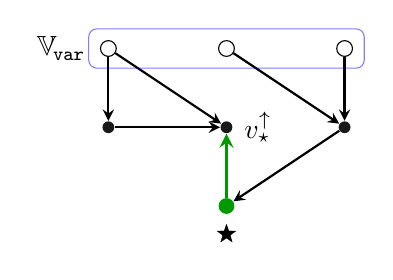
\begin{tikzpicture} 
			[dot/.style={circle,fill=black!90,inner sep=0pt, minimum size=1.5mm},
				empty/.style={inner sep=0pt, minimum size=1.5mm},
				spine/.style={very thick},
				edge/.style={thick}]
			\begin{scope}
				%\node[rectangle,draw=blue!50,rounded corners=3pt,minimum width=12mm, minimum height=5mm] at (0.15,1) {};
				\node[rectangle,draw=blue!50,rounded corners=3pt,minimum width=35mm, minimum height=5mm] at (0,2) {};

				\node at (0,0)  [root,label=below:$\STAR$] (zero) {};
				\node at (-1.5,1) [dot] (left) {};
				\node at (0.4,1) {$v_{\star}^\uparrow$};
				\node at (0,1) [dot] (up) {};
				\node at (1.5,1) [dot] (right) {};
				%\draw[->,spine, color=testcolor] (zero) to node [sloped,below] {} (left);
				\draw[->,spine, color=testcolor] (zero) to node [sloped,below] {} (up);
				\draw[->,edge] (right) to node [sloped,below] {} (zero);
				\draw[->,edge] (left) to node [sloped,below] {} (up);

				\node at (-1.5,2) [var] (up_left) {};
				\node at (-2.1,2) {$\CCV_{\!\var}$};
				\node at (0,2) [var] (up_up) {};
				\node at (1.5,2) [var] (up_right) {};

				\draw[->,edge] (up_left) to node [sloped,below] {} (left);
				\draw[->,edge] (up_left) to node [sloped,below] {} (up);
				\draw[->,edge] (up_up) to node [sloped,below] {} (right);
				\draw[->,edge] (up_right) to node [sloped,below] {} (right);
			\end{scope}
		\end{tikzpicture}
		\caption{An example of the graph $\CCG$, where the green edge connects the distinguished vertices $\protect\STAR$ and $v_{\star}^{\uparrow}$. The white vertices are in $\CCV_{\!\var}$ and have only outgoing edges. The distinguished vertex $\protect\STAR$ has an incoming edge, but it cannot come from $v_{\star}^{\uparrow}$.}
		\label{fig:graph}
	\end{figure}

Using the notation of Section~\ref{sec:contractions}, we write $\fC(\CCV_{\!\var})$ for the set of all contractions on $\CCV_{\!\var}$. For a graph $\CCG = (\CCV,\CCE)$ and a contraction $\gamma \in \fC(\CCV_{\!\var})$ we define the multigraph (i.e. two vertices are allowed to be connected by multiple edges) $\CCG_\gamma = (\tilde \CCV, \tilde\CCE)$, with labels $(\tilde a_e, \tilde r_e)$, in the following way: the set of vertices $\tilde \CCV \subset \CCV$ is obtained from $\CCV$ by identifying those vertices from $\CCV_{\!\var}$ which belong to the same component in $\gamma$. We denote this ``identification'' by a surjective map $\i_\gamma : \CCV \to \tilde \CCV$. In particular, $\i_\gamma$ maps the vertices from $\CCV \setminus \CCV_{\!\var}$ (which includes $\STAR$) to themselves. We define $\tilde \CCV_{\!\var}$ to be the image of $\CCV_{\!\var}$ under the map $\i_\gamma$. Then we define the set of edges $\tilde \CCE$ on $\tilde \CCV$ to contain $\tilde e = (\i_\gamma(e_-), \i_\gamma(e_+))$ for all $e = (e_-, e_+) \in \CCE$, with the label $(a_{\tilde e}, r_{\tilde e}) = (a_e, r_e)$. In what follows, we call $\CCG_\gamma = (\tilde \CCV, \tilde \CCE)$\label{lab:contracted_graph} the {\it contracted (multi)graph} corresponding to $\CCG$ and $\gamma$. To consider renormalised integrals, we will use a labeling $\L$ of the components of the contraction $\gamma$, defined as in Section~\ref{sec:renormalized-integrals}. We by analogy with \eqref{eq:Gamma-set} we define the set of vertices  %By analogy with \eqref{eq:Gamma-sets}, 
\begin{equation}\label{eq:Gamma-sets-V}
\Gamma := \{ v \in \tilde{\CCV}_{\!\var} :  |\i_\gamma^{-1}(v)| = 1 \} \cup \L^{-1}(\diamond),
%	 \Gamma_{\!1, \diamond} &:= \{ v \in \tilde{\CCV}_{\!\var} :  |\i_\gamma^{-1}(v)| = 1 \} \cap \L^{-1}(\diamond),
%	 \Gamma_{2} &:= \{ v \in \tilde{\CCV}_{\!\var} :  |\i_\gamma^{-1}(v)| = 2 \}.
\end{equation}
which correspond to the variables integrated with respect to martingales. 
%and we will use the shorthand $\Gamma_{\!1, \diamond}^c := \tilde{\CCV}_{\!\var} \setminus \Gamma_{\!1, \diamond}$.

A special case is $\CCV_{\!\var} = \emptyset$, in which all the definitions in the previous paragraph make sense for the identity contraction $\gamma = \id$, and the contracted graph $\CCG_\gamma$ coincides with the original one $\CCG$. 

It will be useful to define a \emph{simple} (containing no multiedges) graph $(\hat \CCV, \hat \CCE)$, such that $\hat \CCV = \tilde \CCV$ and the unique edge $e \in \hat \CCE$ from $e_-$ to $e_+$ is obtained by contracting all edges $\tilde e$ from $e_-$ to $e_+$ in $\tilde \CCE$, with the label $(\hat a_e, r_e)$ of $e$ being the sum of the labels of all such parallel edges $\tilde e$. It follows from Assumption~\ref{a:mainGraph} that if there is more than one edge connecting $e_-$ to $e_+$ in $\CCG_\gamma$, then the value $r_e$ associated to the contracted edge is either $0$ (if all these edges $\tilde e \in \tilde \CCE$ have $r_{\tilde e} = 0$), or coincides with the only value $r_{\tilde e} > 0$, for $\tilde e \in \tilde \CCE$ connecting $e_-$ to $e_+$. We can have $r_e < 0$ only if there is a unique edge $\tilde e$ from $e_-$ to $e_+$ with $r_{\tilde e} < 0$.

For a subset $\bar\CCV \subset \CCV$ we define the outgoing edges $\CCE^\uparrow (\bar \CCV) := \{e \in  \CCE : e_- \in \bar\CCV\}$, incoming edges $ \CCE^\downarrow (\bar \CCV) := \{ e\in  \CCE : e_+ \in \bar\CCV\}$, internal edges $ \CCE_0 (\bar \CCV) := \{e \in  \CCE : e_{\pm} \in \bar \CCV\}$, and incident edges $ \CCE (\bar \CCV) := \{e \in  \CCE : e_{-} \in \bar \CCV \text{ or } e_{+} \in \bar \CCV\}$. If $\bar \CCV =  \CCV$, we simply write $ \CCE^\uparrow$, $ \CCE^\downarrow$, etc. Furthermore, we define the sets $\CCE_+ (\bar \CCV) := \{e \in  \CCE(\bar \CCV) :  r_e > 0\}$, $ \CCE_- (\bar \CCV) := \{e \in  \CCE(\bar \CCV) :  r_e < 0\}$, $ \CCE_+^\uparrow :=  \CCE_+ \cap  \CCE^\uparrow$ and $ \CCE_+^\downarrow :=  \CCE_+ \cap  \CCE^\downarrow$. These sets, defined for the edges $\tilde \CCE$ and $\hat \CCE$, will have the respective decorations. 

Then we require the contracted graph to satisfy the following assumption, which we state for the simple graph $(\hat \CCV, \hat \CCE)$ defined above. 

\begin{assumption}\label{a:mainContraction}
	The graph $\CCG = (\CCV,\CCE)$ and the contraction $\gamma \in \fC(\CCV_{\!\var})$ are such that the graph $(\hat \CCV, \hat \CCE)$, defined above, has the following properties:
	\begin{enumerate}[topsep=2pt, itemsep=0ex]
		\item\label{it:mainContraction-1} for any edge $e \in \hat\CCE$ one has $\hat a_e + (r_e \wedge 0) < |\s|$;
		\item\label{it:mainContraction-2} for every subset $\bar \CCV \subset \hat \CCV_{\!\bar\star}$ of cardinality at least $3$ one has
		      \begin{equation*}
			      \sum_{e  \in \hat\CCE_0(\bar \CCV)} \hat a_e < \Bigl(2 |\bar \CCV| - |\bar \CCV \cap \Gamma| - 1 - \1_{\bar \CCV \cap \Gamma = \emptyset} \Bigr) \frac{|\s|}{2};
		      \end{equation*}
		\item for every subset $\bar \CCV \subset \hat \CCV$ containing $\STAR$ of cardinality at least $2$ one has
		      \begin{equation*}
			      \sum_{e \in \hat \CCE_0 (\bar \CCV)} \hat a_e + \sum_{e \in \hat \CCE^{\uparrow}_+ (\bar \CCV)} \bigl(\hat a_e + r_e - 1\bigr) - \sum_{e \in \hat \CCE^{\downarrow}_+ (\bar \CCV)} r_e < \Bigl(2 |\bar \CCV| - |\bar \CCV \cap \Gamma| \Bigr) \frac{|\s|}{2};
		      \end{equation*}
		\item for every non-empty subset $\bar \CCV \subset \hat \CCV_{\!\bar\star} \setminus \{ v_{\star}^\uparrow \}$ one has
		      \begin{equation*}
			      \sum_{e \in \hat \CCE(\bar \CCV) \setminus \hat \CCE^{\downarrow}_+(\bar \CCV)} \hat a_e + \sum_{e \in \hat \CCE^{\uparrow}_+(\bar \CCV)} r_e - \sum_{e \in \hat \CCE^\downarrow_+(\bar \CCV)}( r_e - 1) > \Bigl(2 |\bar \CCV| - |\bar \CCV \cap \Gamma| \Bigr) \frac{|\s|}{2}.
		      \end{equation*}
	\end{enumerate}
\end{assumption}

\begin{remark}
Assumption~\ref{a:mainContraction} coincides with Assumption~3.17 in \cite{ChandraShen} on an ``elementary graph'',  where the set of ``external vertices'' (see Definition~3.13 in \cite{ChandraShen}) is given in our case by the set $\Gamma$.
\end{remark}


\subsection{Kernels associated to the graph}

Given a graph $\CCG = (\CCV,\CCE)$ as above, to each edge we associate a kernel and each vertex corresponds to a variable in the domain $\R^{d+1}$. Then, for $e \in \CCE$, the values $a_e$ will describe the order of singularity of the kernel associated to the edge $e$. The value $r_e$ will describe the order of renormalisation of this kernel. %Integration will be performed with respect to measures, for which the following assumption holds.
For every vertex $v \notin \CCV_{\!\var} \cup \{\STAR\}$ we assume to be given a measure $\mu^\eps_v$ on $\R^{d+1}$ of the form
\begin{equation}\label{eq:point-measure}
	\mu^\eps (\d z) = \eps^d \sum_{y \in (\eps \Z)^d}  \delta(y - x)\, \d t\, \d x, 
\end{equation}
where $z = (t, x)$ with $t \in \R$ and $x \in \R^{d}$, and where $\delta$ is the Dirac delta function on $\R^d$. This measure counts the points in the space lattice and is the Lebesgue measure in time.
Notice that, as $\eps \to 0$, the measure $\mu^{\eps}_v$ converges locally in weak-$*$ topology to the Lebesgue measure on $\R^{d+1}$.

For each edge of the graph we associate a kernel with the following properties.

\begin{assumption}\label{a:Kernels}
 For every $e \in \CCE$ we consider a smooth\footnote{In all our applications it is sufficient to have kernels sufficiently many times differentiable. For example, we can take them to be in $\SC^q_\s$ for $q = \sum_{e \in \CCE} (|r_e| + 2)$.} kernel $K^{\eps}_e \colon \R^{d+1} \to \R$, which can be written as $K^{\eps}_e(z) = \sum_{n = 0}^{N} K^{\eps, n}_{e}(z)$ for $N = - \lfloor \log_2 \epsEH \rfloor$ and for some $\epsEH \in [\eps,1]$, where the smooth functions $\{K^{\eps, n}_{e}\}_{0 \leq n \leq N}$ have the following properties:
	\begin{enumerate}[topsep=2pt, itemsep=0ex]
		\item\label{a:DKernels_support} the function $K^{\eps, n}_{e}(z)$ is supported in $C_1 2^{-n} \leq \|z\|_\s \leq C_2 2^{-n}$ for some $0 < C_1 < C_2$;
		\item\label{a:DKernels_bounds} for any $q \geq 0$ and for some $C > 0$, independent of $\eps$ and $\epsEH$, one has
		      \begin{equation}\label{eq:Kn_bound}
			      |D^k K^{\eps, n}_{e}(z)| \leq C 2^{n(a_e + |k|_\s)}\;,
		      \end{equation}
		      uniformly in $z$, $|k|_\s \leq q$ and $0 \leq n \leq N$;
		\item\label{a:DKernels_poly} if $r_e < 0$, then for all $0 \leq n \leq N$ and $|k|_\s < |r_e|$ one has 
		\begin{equation}\label{eq:Kn_killer}
			\int_{\R^{d+1}} z^k K^{\eps, n}_{e}(z) \mu_{e_+}^{\eps}(\d z) = 0.
		\end{equation}
	\end{enumerate}	
\end{assumption}

The necessity to introduce a new parameter $\epsEH$ can be seen in our application in Section~\ref{sec:applicationStochQuant}, where the mesh size of the grid is $\eps$ and the interaction range is defined on the scale $\eps^{\frac{3}{4}} \geq \eps$.

We see from \eqref{eq:Kn_bound} that the value $a_e$ characterizes the order of singularity of the kernel. Moreover, the value $r_e$, assigned to an edge $e \in \CCE$, describes a renormalisation of the singularity, which for positive and negative values are defined in different ways (see the following section).

\begin{lemma}\label{lem:K_bound}
	 If Assumption~\ref{a:Kernels} is satisfied, then for any $q \geq 0$, the following quantity is bounded uniformly in $\epsEH \in [\eps,1]$ and $\eps \in (0, 1]$
	\begin{equation}\label{eq:K_bound}
					\| K^{\eps}_e \|^{(\epsEH)}_{a_e; q} := 
					\sup_{z \in \R^{d+1}} \sup_{|k|_\s < q} (\|z\|_\s + \epsEH)^{a_e + |k|_\s} |D^k K^{\eps}_{e}(z)|.
	\end{equation}
	The reverse statement if also true, i.e. if a kernel $K^{\eps}_e$ satisfies the bound \eqref{eq:K_bound} holds, then it has all the properties listen in Assumption~\ref{a:Kernels}. 
\end{lemma}

\begin{proof}
	The bound \eqref{eq:K_bound} is a direct consequence of Assumption~\ref{a:Kernels}\eqref{a:DKernels_support}-\eqref{a:DKernels_bounds}. The second part of the lemma follows by repeating the proof of \cite[Lemma~5.4]{HM18}.
\end{proof}

\subsubsection{Renormalisation}
\label{sec:renormalisation}

If $r_e \neq 0$, then the kernel corresponding to the edge $e$ requires renormalisation. For positive and negative values of $r_e$ the renormalisation is defined different. For $r_e > 0$ the renormalisation of the smooth kernel is required to get a sufficiently fast decay of the kernel at the origin. In the case $r_e < 0$ the renormalisation is required to make the kernel, with a very strong singularity at the origin, integrable. 

In the case $r_e > 0$, we define the renormalised kernel
\begin{equation}\label{e:defKhatn2}
	\hat K^{\eps}_e(z_{e_-}, z_{e_+}) := K^{\eps}_e(z_{e_+}-z_{e_-}) - \sum_{|k|_\s < r_e} {z_{e_+}^k \over k!} D^k K^{\eps}_e(-z_{e_-}),
\end{equation}
where the sum runs over all multi-indices $k \in \N_0^{d+1}$ such that $|k|_\s < r_e$. In the case $r_e = 0$ we simply define $\hat K^{\eps}_e(z_{e_-}, z_{e_+}) := K^{\eps}_e(z_{e_+}-z_{e_-})$. The positive renormalisation \eqref{e:defKhatn2} allows to define kernels, which have sufficiently fast polynomial decay at the diagonal $z_{e_-} = z_{e_+}$. This is the case when $K^{\eps}_e$ is smooth with uniformly bounded derivatives.

If $r_e < 0$, then for a smooth and compactly supported function $\phi$ on $\R^{d+1} \times \R^{d+1}$ we define the expansion
\begin{equation}\label{e:Taylor}
	(T_{r_e} \phi)(z_{e_-}, z_{e_+}) := \phi(z_{e_-}, z_{e_+}) - \sum_{|k|_\s < |r_e|} {(z_{e_+} - z_{e_-})^k \over k!} D_2^k \phi(z_{e_-}, z_{e_-}),
\end{equation}
where the sum runs over all multi-indices $k \in \N_0^{d+1}$ satisfying $|k|_\s < |r_e|$, and where $D_2^k$ is the multi-derivative in the second argument. Furthermore, we associate to $K^{\eps}_e$ the distribution
\begin{align}\label{e:defRen}
	\hat{K}^{\eps}_e(\phi) := \int_{\R^{d+1}} \int_{\R^{d+1}} \!K^{\eps}_e(z_{e_+} - z_{e_-}) (T_{r_e} \phi)(z_{e_-}, z_{e_+})\,\mu^{\eps}_{e_-}(\d z_{e_-}) \mu^{\eps}_{e_+}(\d z_{e_+}),
\end{align}
which is obtained from $K^{\eps}_e$ by subtracting delta-functions and their derivatives. Expression \eqref{e:defRen} is just another way to write the integral
\begin{equation*}
	\int_{\R^{d+1}} \int_{\R^{d+1}} \!K^{\eps}_e(z_{e_+} - z_{e_-}) \phi(z_{e_-}, z_{e_+})\,\mu^{\eps}_{e_-}(\d z_{e_-}) \mu^{\eps}_{e_+}(\d z_{e_+}),
\end{equation*}
since $\int_{\R^{d+1}} \!K^{\eps}_e(z) z^k\, \mu^{\eps}_{e_+}(\d z) = 0$ and the measure $\mu^{\eps}_{e_+}$ is translation invariant. %In particular, we will be interested in the cases when this double-integral is not bounded uniformly in $\eps \geq \eps$, but the expression \eqref{e:defRen} is.

\begin{remark}
	In all of the applications that we have in mind, we deal with labels $r_e$ which are either $+1$, $0$ or $-1$. In Section~\ref{sec:applicationStochQuant}, for example, we have $r_e = 1$ only for the tree in Section \ref{sec:last_symbol}; we use negative renormalisation with $r_e = -1$ only for the tree which is dealt with in \eqref{eq:important_subtree}. All the other edges in the trees of Section~\ref{sec:applicationStochQuant} always have $r_e=0$.
	
	Clearly, when $r_e =0$, we have no transformation to do on the kernels. When $r_e = 1$, on the other hand, we have \[ \hat K^{\eps}_e(z_{e_-}, z_{e_+}) := K^{\eps}_e(z_{e_+}-z_{e_-}) - K^{\eps}_e(-z_{e_-}), \] while when $r_e = -1$, we get \[ \hat K^{\eps}_e(z_{e_-}, z_{e_+}) := K^{\eps}_e(z_{e_+}-z_{e_-}) - \left( \int K^{\eps}_e(z_{e_+} - z_{e_-}) \mu^{\eps}_{e_+}(\d z_{e_+}) \right) \delta(z_{e_+}-z_{e_-}), \] where $\delta$ is the Dirac delta-function. Observe that positive renormalisation corresponds to subtracting the value of the kernel itself at the ``base'' point $z_{e_{-}}$, while negative renormalisation means removing singularities at the base point.
\end{remark}

\subsubsection{A generalised convolution}

Let us fix a graph $\CCG = (\CCV,\CCE)$ as described above. Then for a smooth and compactly supported function $\phi : \R^{d+1} \to \R$, for $z = (t, x), \bar z = (\bar t, \bar x) \in \R^{d+1}$ and for $\lambda \in (0,1]$ we define its rescaling and recentering
\begin{equation}\label{eq:test-function}
	\phi^\lambda_{\bar z}(z) := \lambda^{-|\s|} \phi \bigl(\lambda^{-2}(t - \bar t), \lambda^{-1}(x - \bar x)\bigr).
\end{equation}
For fixed $\bz^{\var} \in (\R^{d+1})^{\CCV_{\!\var}}$ we define the product measure on $\bz \in (\R^{d+1})^{\CCV_{\!\bar\star}}$
\begin{equation}\label{e:mu_def}
	\mu_{\CCV_{\!\bar\star}, \bz^{\var}}^{\eps}(\d \bz) := \Bigl(\prod_{v \in \CCV_{\!\bar\star} \setminus \CCV_{\!\var}} \mu_v^{\eps}(\d z_v)\Bigr) \Bigl(\prod_{w \in \CCV_{\!\var}} \delta(z_w - z^{\var}_w) \d z_w\Bigr),
\end{equation}
where again $\delta$ is the Dirac delta-function, and where $\bz = (z_v \in \R^{d+1} : v \in \CCV_{\!\bar\star})$ and $\bz^{\var} = (z^{\var}_v \in \R^{d+1} : v \in \CCV_{\!\var})$. In other words, the variable $z_v$, corresponding to the vertex $v \in \CCV_{\!\bar\star} \setminus \CCV_{\!\var}$, is integrated with respect to the measures $\mu_v^{\eps}$, and the variables corresponding to the vertices in $\CCV_{\!\var}$ are fixed to be equal to $\bz^{\var}$. These are the variables which we want to integrate with respect to martingales. Then we define the \emph{generalised convolution}
\begin{equation}\label{e:genconv}
	\CK^{\lambda, \eps}_\CCG(\bz^{\var}) := \int_{(\R^{d+1})^{\CCV_{\!\bar\star}}} \Bigl( \prod_{e\in \CCE}{\hat K}^{\eps}_e(z_{e_-}, z_{e_+})\Bigr) \phi^\lambda_0(z_{v_{\star}^\uparrow}) \mu_{\CCV_{\!\bar\star}, \bz^{\var}}^{\eps}(\d \bz).
\end{equation}
Since the kernels $K^{\eps}_e$ are smooth, our assumptions on the graph guarantee that the generalised convolution \eqref{e:genconv} is well-defined.


We fix any order of the elements in $\CCV_{\!\var}$ (which respectively fixed the order of the variables in $\CK^{\lambda, \eps}_\CCG(\bz^{\var})$) and we define 
\begin{equation} \label{eq:def_integrals_kernels}
	(\CI^{\eps, \L}_{\gamma} \CK^{\lambda, \eps}_\CCG )_t := \sum_{\sigma \in \Sigma_\ga} (\CI^{\eps, \L}_{\gamma, \sigma} \CK^{\lambda, \eps}_\CCG )_t,
\end{equation}
where the stochastic integral $\CI^{\eps, \L}_{\gamma, \sigma}$ is defined in Section~\ref{sec:renormalized-integrals} with respect to the fixed order of the variables. The following is our main result of this section.
\begin{theorem}\label{thm:convolutions}
	Let $\CCG=(\CCV,\CCE)$ be a graph with labels $\{a_e,r_e\}_{e\in \CCE}$ satisfying Assumption~\ref{a:mainGraph}, let $\gamma \in \fC_m(\CCV_{\!\var})$, with $1 \leq m \leq |\CCV_{\!\var}|=n$, be a contraction with a labeling $\L$ such that Assumption~\ref{a:mainContraction} is satisfied. Let the measures be defined as in \eqref{eq:point-measure} and let the kernels satisfy Assumption~\ref{a:Kernels}. 
	Let furthermore $\CI^{\eps, \L}_{\gamma}$ be a stochastic integral with respect to \cadlag martingales satisfying Assumption~\ref{a:Martingales}, let the set $\Gamma$ be defined in \eqref{eq:Gamma-sets-V}, and let 
	\begin{equation}\label{eq:alpha-gamma}
		\nu_\gamma := |\s| |\hat \CCV_{\!\bar\star} \setminus \{ \hat{v}^\uparrow_{\!\star} \}| - \frac{|\s|}{2} | \Gamma|  - \sum_{e \in \hat \CCE} \hat a_e < 0. 
	\end{equation}
	Then for any $\bar \kappa > 0$ there is $p_* \geq 2$ such that for every $p \geq p_*$ there is a constant $C$ for which the following bound holds
	\begin{align}\label{e:genconvBound}
		\biggl(\E \biggl[\sup_{t \in \R_+} \bigl| (\CI^{\eps, \L}_{\gamma} \CK^{\lambda, \eps}_\CCG)_t \bigr|^p\biggr]\biggr)^{\frac{1}{p}} &\le C (\lambda \vee \epsEH)^{\nu_\gamma} \sum_{A \sqcup B = \tilde \CCV_{\!\var}} \eps^{\alpha_\gamma(A, B)} \epsEH^{- \beta_{\gamma}(A, B)} \\
		&\qquad + C (\lambda \vee \epsEH)^{\nu_\gamma} \sum_{A \sqcup B \subsetneq \tilde \CCV_{\!\var}} \eps^{\alpha_\gamma(A, B) - \bar \kappa} \epsEH^{- \beta_{\gamma}(A, B)} \nonumber
	\end{align}
	uniformly in $\lambda \in (0,1]$, $\epsEH \in [\eps, 1]$ and $\eps \in (0,1]$, where the sums run over disjoint subsets $A$ and $B$ of $\tilde \CCV_{\!\var}$, such that $\L^{-1}(\triangledown) \subseteq B$ and $B \cap \Gamma = \emptyset$, the constant $\alpha_\gamma(A, B)$ is defined in \eqref{eq:alpha-power}, where
	\begin{equation}\label{eq:beta-constant}
	\beta_{\gamma}(A, B) := \frac{|\s|}{2} \Bigl( |A \setminus \Gamma| + 2 |(A \sqcup B)^c \setminus \Gamma | + |(A \sqcup B)^c \cap \Gamma |\Bigr),
	\end{equation}
	and with $(A \sqcup B)^c = \tilde \CCV_{\!\var} \setminus (A \sqcup B)$.
\end{theorem}

We prove this theorem in Section~\ref{sec:proof_bound}, and before that we need to get some preliminary results. 

\begin{remark}
From the proof of Theorem~\ref{thm:convolutions} we can see that there exists a value $q \geq 0$ and a compact set $\fK \subset \R^{d+1}$, such that the constant $C$ in \eqref{e:genconvBound} is proportional to
\begin{equation*}
\Bigl(\prod_{e \in \CCE} \| K^{\eps}_e \|^{(\epsEH)}_{a_e; q} \Bigr) \Bigl(\prod_{v \notin \CCV_{\!\var} \cup \{\star\}} \| \mu^{\eps}_{v} \|_{\TV(\fK)} \Bigr),
\end{equation*}
which by our assumptions is bounded uniformly in $\eps$ and $\epsEH$. For example, we can take a very rough value $q = \sum_{e \in \CCE} (|r_e| + 2)$.
\end{remark}

If we would like to consider a recentered test function $\phi^\lambda_{\bar z}(z)$, we need to shift respectively all the variables in the generalised convolution:
\begin{equation}\label{e:genconv_shift}
	\CK^{\lambda, \eps}_{\CCG, \bar z}(\bz^{\var}) := \int_{(\R^{d+1})^{\CCV_{\!\bar\star}}} \Bigl(\prod_{e\in \CCE}{\hat K}^{\eps}_e(z_{e_-} - \bar z, z_{e_+} - \bar z)\Bigr) \phi^\lambda_{\bar z}(z_{v_{\star}^\uparrow}) \mu_{\CCV_{\!\bar\star}, \bz^{\var}}^{\eps}(\d \bz).
\end{equation}
Then the following result can be proved as Theorem~\ref{thm:convolutions}, by changing the value of the variable $z_{\star}$ from $0$ to $\bar z$. Uniformity in $\bar z$ holds, because the norms of the kernels \eqref{e:wantedBound4} are independent of this variable. 

\begin{corollary}\label{cor:convolutions}
Under the assumptions of Theorem~\ref{thm:convolutions}, the bound \eqref{e:genconvBound} holds for the multiple integral $\CI^{\eps, \L}_\gamma \CK^{\lambda, \eps}_{\CCG, \bar z}$, locally uniformly in $\bar z$. 
%Moreover, the limit \eqref{eq:integrals-convergence} holds, where the variables in the limiting kernel are shifted by $\bar z$. 
\end{corollary}

Applying Minkowski inequality, we get from the definition \eqref{eq:def_integrals_kernels} the bound 
\begin{equation}\label{eq:integral-and-sigmas}
\biggl(\E \biggl[\sup_{t \in \R_+} \bigl| (\CI^{\eps, \L}_{\gamma} \CK^{\lambda, \eps}_\CCG)_t \bigr|^p\biggr]\biggr)^{\frac{1}{p}} \leq \sum_{\sigma \in \Sigma_\ga} \biggl(\E \biggl[\sup_{t \in \R_+} \bigl| (\CI^{\eps, \L}_{\gamma, \sigma} \CK^{\lambda, \eps}_\CCG)_t \bigr|^p\biggr]\biggr)^{\frac{1}{p}}.
\end{equation}
In the rest of the section we are going to prove the bound \eqref{e:genconvBound} only for the integral $\CI^{\eps, \L}_{\gamma, \imath}$ with the trivial permutation of the variables $\imath$, defined in Section~\ref{sec:orderings_vars}. One can see from the proof, that this bound is independent of the order of the variables (although the order plays a role in some intermediate results like Lemma~\ref{lem:KTildeBound}), and the same bound \eqref{e:genconvBound} follows for every integral $\CI^{\eps, \L}_{\gamma, \sigma}$.

\subsection{Multiscale decomposition of the generalised convolution}
\label{sec:decomp}

Our aim is to write the kernels $K_e^{\eps}$ in the generalised convolution \eqref{e:genconv} as sums of localised functions. For the edge $(\star, v_{\star}^\uparrow)$, we view the test function $\phi^\lambda_0(z_{v_{\star}^\uparrow})$ in \eqref{e:genconv} as a new kernel $K_{(\star, v_{\star}^\uparrow)}(z_{v_{\star}^\uparrow})$, supported on $\| z_{v_{\star}^\uparrow} \|_\s \lesssim \lambda$ and satisfying $\| K_{(\star, {v_{\star}^\uparrow})} \|_{0; q} \lesssim \lambda^{-|\s|}$ (recall that this edge has the labels $a_e = r_e = 0$ in the graph).

Our next aim is to decompose the kernels in \eqref{e:genconv} into sums of localised functions. To this end, for $e \in \CCE$ with $r_e > 0$, we take any smooth functions $\psi^{(\eps, n)} : \R^{d+1} \to \R$, such that $\psi^{(\eps, n)}(z)$ is supported in $C_1 2^{- n} \leq \|z\|_\s \leq C_2 2^{-n}$ (where $C_1, C_2$ are from Assumption~\ref{a:Kernels}), scales as $2^{-n}$ and satisfies $\sum_{n = 0}^N \psi^{(\eps, n)}(z) = 1$ for all $z$. Let us denote for convenience $\N_{\leq N} := \{0,1,\ldots, N\}$.\label{lab:NN} Then for $r_e > 0$ and $\n = (k,p,m) \in \N_{\leq N}^3$ we set
\begin{equation}\label{e:defKhatn}
	\hat K_e^{\eps, \n}(z,\bar z) := \psi^{(\eps, k)}(\bar z-z) \psi^{(\eps, p)}(z) \psi^{(\eps, m)}(\bar z) \hat K_e^{\eps}(z,\bar z),
\end{equation}
where the kernel $\hat K^{\eps}_e$ has been defined in \eqref{e:defKhatn2}. For $\n \in \N_{\leq N}^3$ and $e \in \CCE$ such that $r_e \leq 0$, we define the function
\begin{equation*}
	\hat K_e^{\eps, \n}(z,\bar z) :=
	\begin{cases}
		K^{\eps, k}_e(\bar z - z), & \text{if}~ \n = (k,0,0),\; 0 \leq k \leq N, \\
		0,                         & \text{otherwise},
	\end{cases}
\end{equation*}
where we made use of the expansion of the kernel from Assumption~\ref{a:Kernels}.

For $\lambda \in (0,1]$ we define the set $\CN^{\epsEH}_{\lambda}$ of functions $\n \colon \CCE \to \N_{\leq N}^3$ satisfying $2^{-|\n_{(\star, v^{\uparrow}_{\star})}|} \le \lambda \vee \epsEH$, 
with $\n_{(\star, v^{\uparrow}_{\star})}$ being the evaluation of the function $\n$ on the edge $(\star, v^{\uparrow}_{\star})$. Then for a function $\n \in \CN^{\epsEH}_{\lambda}$ and a point $\bz = (z_v : v \in \CCV_{\!\bar \star})$, we define
\begin{equation}\label{def:kayhat}
	\hat K^{\eps, \n}(\bz) := \prod_{e \in \CCE} \hat K_e^{\eps, \n_e}(z_{e_-}, z_{e_+}),
\end{equation}
where $z_\star = 0$. Since the functions $\psi^{(\eps, n)}$ sum up to $1$ and since we consider the test function $\phi^\lambda_0$ as a kernel, one can rewrite the generalised convolution \eqref{e:genconv} as
\begin{equation}\label{e:bigsum}
	\CK^{\lambda, \eps}_\CCG(\bz^{\var}) := \sum_{\n \in \CN^{\epsEH}_{\lambda}} \CK^{\eps, \n}_\CCG(\bz^{\var}), \qquad  \CK^{\eps, \n}_\CCG(\bz^{\var}) := \int_{(\R^{d+1})^{\CCV_{\!\bar\star}}} \!\!{\hat K}^{\eps, \n}(\bz)\, \mu_{\CCV_{\!\bar\star}, \bz^{\var}}^{\eps}(\d \bz).
\end{equation}

Since we are interested in estimating the integrals $\CI^{\eps, \L}_{\gamma, \imath} \CK^{\lambda, \eps}_\CCG$, we can exploit the fact that the integration variables $z_v$ in the kernel \eqref{e:bigsum}, for vertices $v$ belonging to the same component of $\gamma$, are equal. More precisely, we define the set $\CN^{\epsEH}_{\lambda, \gamma}$ in the same way as $\CN^{\epsEH}_{\lambda}$, but using the contracted graph $\CCG_\gamma = (\tilde \CCV, \tilde \CCE)$. Then for a function $\n \in \CN^{\epsEH}_{\lambda, \gamma}$ and a point $\bz = (z_v : v \in \tilde \CCV_{\!\bar \star})$, we define the kernel $\hat K^{\eps, \n}(\bz)$ as in \eqref{def:kayhat}, but with the product over $\tilde \CCE$. Furthermore, we define the measure $\mu_{\tilde \CCV_{\!\bar \star}, \bz^{\var}}^{\eps}$ on $(\R^{d+1})^{\tilde \CCV_{\!\bar\star}}$ by
\begin{equation}\label{eq:measure-mu-general}
	\mu_{\tilde \CCV_{\!\bar \star}, \bz^{\var}}^{\eps}(\d \bz) := \Bigl(\prod_{v \in \tilde \CCV_{\!\bar\star} \setminus \tilde \CCV_{\!\var}} \mu_v^{\eps}(\d z_v)\Bigr) \Bigl(\prod_{w \in \tilde \CCV_{\!\var}} \delta_{z_w - z^{\var}_{w_*}} \d z_w\Bigr),
\end{equation}
where $w_*$ is the first element (with respect to a chosen order of vertices) in $\i_\gamma^{-1}(w)$, and the map $\i_\gamma$ has been introduced in the beginning of this section. In other words, this measure identifies the variables in $\tilde \CCV_{\!\var}$ which correspond to the same component of $\gamma$. Then we define the kernel
\begin{equation}\label{e:Kernel_hat}
	\CK^{\eps, \n}_{\CCG_\gamma}(\bz^{\var}) := \int_{(\R^{d+1})^{\tilde \CCV_{\!\bar\star}}} \!\!{\hat K}^{\eps, \n}(\bz)\, \mu_{\tilde \CCV_{\!\bar \star}, \bz^{\var}}^{\eps}(\d \bz),
\end{equation}
and write the multiple stochastic integral as $\CI^{\eps, \L}_{\gamma, \imath} \CK^{\lambda, \eps}_\CCG = \sum_{\n \in \CN^{\epsEH}_{\lambda, \gamma}} \!\!\CI^{\eps, \L}_{\gamma, \imath} \CK_{\CCG_\gamma}^{\eps, \n}$. Using this expansion and applying Minkowski's inequality, we obtain the bound
\begin{equation}\label{e:wantedBound2}
	\biggl(\E \biggl[\sup_{t \in \R_+} \bigl| (\CI^{\eps, \L}_{\gamma, \imath} \CK^{\lambda, \eps}_\CCG)_t \bigr|^p\biggr]\biggr)^{\frac{1}{p}} \leq \sum_{\n \in \CN^{\epsEH}_{\lambda, \gamma}} \biggl(\E \biggl[\sup_{t \in \R_+} \bigl|(\CI^{\eps, \L}_{\gamma, \imath} \CK_{\CCG_\gamma}^{\eps, \n})_t \bigr|^p\biggr]\biggr)^{\frac{1}{p}}.
\end{equation}
Bounding a multiple integral of the generalised convolution boils down to bounding integrals in \eqref{e:wantedBound2} and summing over the functions $\n \in \CN^{\epsEH}_{\lambda, \gamma}$. This is what we do in the next sections, where, following the idea of \cite[Appendix~A.2]{HQ18}, we use a multiscale clustering in the sum over $\n$.

\subsection{Bounds on iterated integrals}
\label{sec:bounds-multiscale}

We associate to every point $\bz \in (\R^{d+1})^{\tilde \CCV}$ a rooted labelled binary tree $(T,\ell)$, such that $\|z_v - z_{w}\|_\s \sim 2^{-\ell_{v \wedge w}}$ and $\ell_{v \wedge w} \in \N_{\leq N}$, where $v \wedge w$ is the closest common ancestor of $v$ and $w$. Moreover, the labels $\ell$ satisfy $\ell_\v \ge \ell_\w$ whenever $\v \ge \w$, where $\v \ge \w$ means that $\w$ belongs to the shortest path from $\v$ to the root of the tree $T$. See \cite[Appendix~A.2]{HQ18} for construction of such tree and also for the terminology which we are going to use. Given a set of vertices $\tilde \CCV$, we denote by $\CCT^{\epsEH}(\tilde\CCV)$  the set of rooted labelled binary trees $(T,\ell)$ as above, which have $\tilde\CCV$ as their set of leaves. Denote furthermore by $\CCT_{\!\lambda}^\epsEH(\tilde\CCV)$ the subset of those labelled trees in $\CCT^{\epsEH}(\tilde\CCV)$ with the property that $2^{-\ell_{\star \wedge v^\uparrow_{\star}}} \le \lambda$. %for any two leaves $v,w \in \{\STAR, v^\uparrow_{\star}\}$.

Our next aim is to write summation in \eqref{e:wantedBound2} over such labelled trees $(T, \ell)$ and then over those functions $\n$ which are close in some sense to the labeling $\ell$. To this end, for the constant $c := (\log_2 |\tilde\CCV|+ |\log_2 C_1|) \vee |\log_2 C_2|$\footnote{Our value of $c$ is different from the analogous value in \cite[Definition~A.8]{HQ18}, because the kernels $K^{\epsEH, n}_{e}$ from Assumption~\ref{a:Kernels} have a different support. The need to define $c$ in this way can be seen from the proof of \cite[Lemma~A.9]{HQ18}.}, where the constants $C_1, C_2$ are from Assumption~\ref{a:Kernels}, we define the set $\CN^{\epsEH}_\gamma(T, \ell)$ consisting of all functions $\n \colon \tilde \CCE \to \N_{\leq N}^3$ such that
\begin{enumerate}[topsep=2pt, itemsep=0ex]
	\item for every edge $e = (v,w)$ with $r_e \le 0$, one has $\n_e = (k,0,0) \in \N_{\leq N}^3$ with $|k - \ell_{v\wedge w}| \le c$,
	\item for every edge $e = (v,w)$ with $r_e > 0$, one has $\n_e = (k,p,m) \in \N_{\leq N}^3$ with $|k - \ell_{v\wedge w}| \le c$, $|p - \ell_{v\wedge \star}| \le c$, and $|m - \ell_{w\wedge \star}| \le c$.
\end{enumerate}
Then we have the following analogue of \cite[Lemma~A.9]{HQ18}, which is proved in exactly the same way.

\begin{lemma}\label{lem:from_n_to_tree}
	Let us fix a point $\bz^{\var} \in (\R^{d+1})^{\CCV_{\!\var}}$. Let $\n \colon \tilde\CCE \to \N_{\leq N}^3$ be such that the kernel $\CK^{\eps, \n}_{\CCG_\gamma}(\bz^{\var})$ defined in \eqref{e:Kernel_hat} does not vanish. Then there exists a labelled tree $(T, \ell) \in \CCT^{\epsEH}_{\!\lambda}(\tilde\CCV)$ such that $\n \in \CN^{\epsEH}_\gamma(T, \ell)$.
\end{lemma}
 
Using this result, the right-hand side of \eqref{e:wantedBound2} can be estimated as
\begin{equation}\label{e:wantedBound3.5}
	\biggl(\E \biggl[\sup_{t \in \R_+} \bigl|(\CI^{\eps, \L}_{\gamma, \imath} \CK^{\lambda, \eps}_\CCG)_t \bigr|^p\biggr]\biggr)^{\frac{1}{p}} \leq \sum_{(T, \ell) \in \CCT^{\epsEH}_{\!\lambda}(\tilde\CCV)} \sum_{\n \in \CN^{\epsEH}_\gamma(T, \ell)} \biggl(\E \biggl[\sup_{t \in \R_+} \bigl|(\CI^{\eps, \L}_{\gamma, \imath} \CK_{\CCG_\gamma}^{\eps, \n})_t \bigr|^p\biggr]\biggr)^{\frac{1}{p}}.
\end{equation}

We will now modify the kernels in \eqref{def:kayhat} in the same way how it was done in \cite[Appendix~A.5]{HQ18}. Let $\Amin \subset \tilde\CCE$ contain those edges $e = (e_-, e_+)$ which have the label $r_e < 0$, and for which any two vertices $\{u,v\}$ satisfying $u \wedge v = e_- \wedge e_+$ coincide with $\{e_-,e_+\}$. Then we can factorize \eqref{def:kayhat} as
\begin{equation}\label{eq:K-hat-A-minus}
	\hat K^{\eps, \n}(\bz) = \hat G^{\epsEH, \n}(\bz) \Bigl(\prod_{e \in \Amin} \hat K_e^{\eps, \n_e}(z_{e_-}, z_{e_+})\Bigr), \qquad \hat G^{\epsEH, \n}(\bz) := \prod_{e \notin \Amin} \hat K_e^{\eps, \n_e}(z_{e_-}, z_{e_+}).
\end{equation}
For $e = (e_-, e_+)$ and $r > 0$ we define the operator $\SY^r_e$ acting on sufficiently smooth functions $V: (\R^{d+1})^{\tilde \CCV} \to \R$ as
\begin{equation*}
	(\SY^r_e V)(\bz) := V(\bz) - \sum_{|k|_\s < r} \frac{(z_{e_+} - z_{e_-})^k}{k!} (D^k_{e_+} V) (P_e(\bz)),
\end{equation*}
where $D^k_{e_+}$ is a derivative with respect to $z_{e_+}$ and where $(P_e(\bz))_v = z_v$ if $v \neq e_+$ and $(P_e(\bz))_v = z_{e_-}$ if $v = e_+$. Furthermore, writing $\Amin = \{e^{(1)}, \ldots, e^{(k)}\}$ for some $k \geq 0$, we define the kernel
\begin{equation}\label{eq:DKernel_tilde}
	\tilde K^{\eps, \n}(\bz) := \Bigl(\SY^{r_{e^{(k)}}}_{e^{(k)}} \cdots \SY^{r_{e^{(1)}}}_{e^{(1)}}\hat G^{\epsEH, \n}(\bz)\Bigr) \Bigl(\prod_{e \in \Amin} \hat K_e^{\eps, \n_e}(z_{e_-}, z_{e_+})\Bigr).
\end{equation}
Then for every $\bz^{\var}$ we have
\begin{equation}\label{eq:two_kernels}
	\int_{(\R^{d+1})^{\tilde\CCV_{\!\bar \star}}} \!\!{\hat K}^{\eps, \n}(\bz)\, \mu_{\tilde\CCV_{\!\bar \star}, \bz^{\var}}^{\eps}(\d \bz) = \int_{(\R^{d+1})^{\tilde\CCV_{\!\bar \star}}} \!\!{\tilde K}^{\eps, \n}(\bz)\, \mu_{\tilde\CCV_{\!\bar \star}, \bz^{\var}}^{\eps}(\d \bz),
\end{equation}
which is just a reformulation of the argument below \cite[Equation~A.26]{HQ18} in our context. Then \eqref{e:wantedBound3.5} can be written as
\begin{equation}\label{e:wantedBound4}
	\biggl(\E \biggl[\sup_{t \in \R_+} \bigl|(\CI^{\eps, \L}_{\gamma, \imath} \CK^{\lambda, \eps}_\CCG)_t \bigr|^p\biggr]\biggr)^{\frac{1}{p}} \leq \sum_{(T, \ell) \in \CCT^{\epsEH}_{\!\lambda}(\tilde\CCV)} \sum_{\n \in \CN^{\epsEH}_\gamma(T, \ell)} \biggl(\E \biggl[\sup_{t \in \R_+} \bigl|(\CI^{\eps, \L}_{\gamma, \imath} \tilde \CK_{\CCG_\gamma}^{\eps, \n})_t \bigr|^p\biggr]\biggr)^{\frac{1}{p}},
\end{equation}
with the new kernels
\begin{equation}\label{e:K_tilde}
	\tilde \CK^{\eps, \n}_{\CCG_\gamma}(\bz^{\var}) := \int_{(\R^{d+1})^{\tilde\CCV_{\!\bar \star}}} \!\!{\tilde K}^{\eps, \n}(\bz)\,\mu_{\tilde\CCV_{\!\bar \star}, \bz^{\var}}^{\eps}(\d \bz).
\end{equation}
Using the notation \eqref{eq:F_gamma}, we denote with $(\tilde \CK^{\eps, \n}_{\CCG_\gamma})^\gamma : (\R^{d+1})^{\tilde\CCV_{\!\var}} \to \R$ the kernel which is obtained from $\tilde \CK^{\eps, \n}_{\CCG_\gamma}$ by making all the variables from the same component of $\gamma$ equal. This is the same definition as in \eqref{eq:F_gamma}. We would like to apply  Theorem~\ref{thm:integral-bound-renorm} to bound the stochastic integrals in \eqref{e:wantedBound4}. For this, we need to estimate the norms \eqref{eq:norm_basis} of the kernel $(\tilde \CK^{\eps, \n}_{\CCG_\gamma})^\gamma(\bz^{\var})$, which is what we are going to do now. 

\medskip
Let $T^\circ$ denote the set of interior nodes of the tree $T$. Then for $e \in \hat E$ let us define the function $\eta_e : T^\circ \to \R$ by
\begin{align*}
	\eta_e(v) & := - \hat{a}_e \1_{e_\uparrow} (v) +  r_e \bigl(\1_{e_+\wedge \star} (v) - \1_{e_\uparrow} (v)\bigr) \1_{ r_e >0,\, e_+\wedge \star > e_\uparrow} \\
	          & \qquad + (1-  r_e -  \hat{a}_e) \bigl(\1_{e_-\wedge \star} (v) - \1_{e_\uparrow} (v)\bigr) \1_{ r_e >0,\, e_-\wedge \star > e_\uparrow},
\end{align*}
where $\1_v(w) := \1_{v = w}$ and $e_\uparrow := e_- \wedge e_+ \in T^\circ$ for an edge $e = (e_-, e_+) \in \hat\CCE$. The function $\eta_e$ coincides with the one defined in \cite[Equation~A.20]{HQ18} and is used to bound the generalised convolution without taking into account negative renormalisation. To consider negative renormalisation we define by analogy with \cite[Equation~A.27]{HQ18} a modified function 
\begin{equation}\label{e:tilde_eta}
	\tilde \eta(v) := |\s| + \sum_{e \in \hat\CCE} \tilde \eta_e(v), \qquad \tilde \eta_e(v) := \eta_e(v) - r_e\, \1_{e \in \Amin} \bigl(\1_{e_\uparrow} (v) - \1_{e_\Uparrow} (v) \bigr),
\end{equation}
where the interior node $e_\Uparrow \in T^\circ$ is of the form $w \wedge e_-$ with $w \not \in e$ which is the furthest from the root. 

From the fixed order of the variables in \eqref{eq:def_integrals_kernels} we obtain an oder of the vertices in $\tilde\CCV_{\!\var}$. Then for every $v \in \tilde\CCV_{\!\var}$ we denote by $v^{\rightarrow}$ the element following after $v$ with respect to this order, and in case when there is no following element we define $v^{\rightarrow} = \STAR$. For $A \subset \tilde \CCV_{\!\var}$, let $T_A$ be the subtree of $T$ containing all the leaves $v$ and $v^{\rightarrow}$, for $v \in A \sqcup \{\STAR\}$, and all the inner nodes $v \wedge v^{\rightarrow}$ for such $v$. Let $T_A^\circ$ contain its inner nodes. 

Then we have the following bound on the norms \eqref{eq:norms-def}-\eqref{eq:norm_basis} of the kernels $(\tilde \CK^{\eps, \n}_{\CCG_\gamma})^\gamma$.

\begin{lemma}\label{lem:KTildeBound}
	Let $\gamma \in \fC_m(\CCV_{\!\var})$ be a contraction with a labeling $\L$, let the set $\Gamma$ be defined in \eqref{eq:Gamma-sets-V}, let $A, B \subseteq \tilde \CCV_{\!\var}$ be disjoint sets such that $B \cap \Gamma = \emptyset$. Then for any labeled tree $(T, \ell) \in \CCT^{\epsEH}_{\!\lambda}(\tilde\CCV)$ and any $p \geq 2$ there is a constant $C$ such that for every $\n \in \CN^{\epsEH}_\gamma(T,\ell)$ one has the bound
	\begin{equation}
		\big\Vert (\tilde \CK^{\eps, \n}_{\CCG_\gamma})^\gamma \big\Vert_{L^{2, 1, p}_\eps(A, B, (A \sqcup B)^c)} \leq C \epsEH^{- \beta_{\gamma, p}(A, B)} \Bigl(\prod_{\nu \in T^\circ} 2^{-\ell_\nu \tilde \eta(\nu)}\Bigr) \Bigl(\prod_{\nu \in T_\Gamma^\circ} 2^{\ell_{\nu}|\s| }\Bigr)^{\frac{1}{2}}, \label{eq:KTildeBound1} 
	\end{equation}
	where we use the norm \eqref{eq:norms-def}-\eqref{eq:norm_basis}, where we write $(A \sqcup B)^c = \tilde{\CCV}_{\!\var} \setminus (A \sqcup B)$, and where 
	\begin{equation}\label{eq:beta-gamma-p}
	\beta_{\gamma, p}(A, B) := |\s| \biggl( \frac{1}{2} |A \setminus \Gamma| + \frac{p-1}{p} |(A \sqcup B)^c \setminus \Gamma | + \frac{p-2}{2 p} |(A \sqcup B)^c \cap \Gamma |\biggr).
	\end{equation}
\end{lemma}

As it was pointed out after the definition \eqref{eq:norms-def}, the norm depends on the chosen order of the variables. The bound \eqref{eq:KTildeBound1} depends on this order through the last multiplier because the set $T_\Gamma^\circ$ is defined using the order. In particular, changing the order of the variables of the kernel in \eqref{eq:KTildeBound1} will change the expression on the right-hand side.

\begin{proof}[of Lemma~\ref{lem:KTildeBound}]
Since each vertex in $\tilde{\CCV}_{\!\var}$ corresponds to a variable with respect to which the norm in \eqref{eq:KTildeBound1} is computed (see the definition \eqref{eq:norms-def}-\eqref{eq:norm_basis}), we choose the order of the vertices in $\tilde{\CCV}_{\!\var}$ to coincide with the order of the variables in the definition of the norm, i.e. we write $\tilde{\CCV}_{\!\var} = (v_1, \ldots, v_M)$.

We are going to prove a more general result; namely, we will prove a bound on the norm of the kernel $(\tilde \CK^{\eps, \n}_{\CCG_\gamma})^\gamma$ some of whose variables are fixed. For this, we take $1 \leq m < M$ and the set $D = \{v_{m+1}, \ldots, v_M\} \subset \tilde \CCV_{\!\var}$ of vertices and we will fix the values of the variables corresponding to these vertices. More precisely, for $\bz_{D} \in (\R^{d+1})^D$ we write $(\tilde \CK^{\eps, \n}_{\CCG_\gamma})^\gamma \big|_{\bz_{D}}$ for the function from $(\R^{d+1})^{\tilde\CCV_{\!\var} \setminus D}$ to $\R$, which is obtained from $(\tilde \CK^{\eps, \n}_{\CCG_\gamma})^\gamma(\bz^{\var})$ by fixing the values of the variables $z^{\var}_v$ with $v \in D$. We extend this definition for $D = \emptyset$ (which corresponds to $m = M$) by $(\tilde \CK^{\eps, \n}_{\CCG_\gamma})^\gamma \big|_{\bz_{\emptyset}} = (\tilde \CK^{\eps, \n}_{\CCG_\gamma})^\gamma$.

For $1 < m \leq M$ and for two disjoint sets $A, B \subseteq \tilde \CCV_{\!\var} \setminus D$, as in the statement of this lemma, we are going to prove the bound
\begin{align}\label{eq:KTildeBound-need}
		&\big\Vert (\tilde \CK^{\eps, \n}_{\CCG_\gamma})^\gamma \big|_{\bz_{D}} \big\Vert_{L^{2, 1, p}_\eps(A, B, (A \sqcup B \sqcup D)^c)} \\
		&\hspace{1cm} \leq C \Bigl(\prod_{\nu \in T^\circ} 2^{-\ell_\nu \tilde \eta(\nu)}\Bigr) \Bigl(\prod_{\nu \in T^\circ_{D}} 2^{\ell_\nu|\s|}\Bigr) \Bigl(\prod_{\nu \in T^\circ_{A}} 2^{\ell_\nu|\s|}\Bigr)^{\frac{1}{2}} \Bigl(\prod_{\nu \in T^\circ_{(A \sqcup B \sqcup D)^c}} 2^{\ell_\nu|\s|}\Bigr)^{\frac{p-1}{p}} \nonumber
\end{align}
uniformly in $\bz_{D} \in (\R^{d+1})^D$, where $(A \sqcup B \sqcup D)^c = \tilde{\CCV}_{\!\var} \setminus (A \sqcup B \sqcup D)$. Moreover, we will show that for $m = 1$ (in which case $D = \CCV_{\!\var}$ and $A = B = \emptyset$) the same bound holds for the absolute value of $(\tilde \CK^{\eps, \n}_{\CCG_\gamma})^\gamma \big|_{\bz_{D}}$.

We can see that the bound \eqref{eq:KTildeBound1} follows from it in the particular case $D = \emptyset$. Indeed, if $D = \emptyset$, then $T^\circ_{D} = \emptyset$ and \eqref{eq:KTildeBound-need} simplifies to
\begin{equation}\label{eq:KTildeBound-need-D-is-empty}
		\big\Vert (\tilde \CK^{\eps, \n}_{\CCG_\gamma})^\gamma \big\Vert_{L^{2, 1, p}_\eps(A, B, (A \sqcup B)^c)} \leq C \Bigl(\prod_{\nu \in T^\circ} 2^{-\ell_\nu \tilde \eta(\nu)}\Bigr) \Bigl(\prod_{\nu \in T^\circ_{A}} 2^{\ell_\nu|\s|}\Bigr)^{\frac{1}{2}} \Bigl(\prod_{\nu \in T^\circ_{(A \sqcup B)^c}} 2^{\ell_\nu|\s|}\Bigr)^{\frac{p-1}{p}}.
\end{equation}
Furthermore, we have $A = (\Gamma \sqcup (A \setminus \Gamma)) \setminus ((A \sqcup B)^c \cap \Gamma)$, where we used our assumption $B \cap \Gamma = \emptyset$, and we write the products over $\nu \in T^\circ_{A}$ as
\begin{equation*}
\prod_{\nu \in T^\circ_{A}} 2^{\ell_{\nu}|\s| }= \Bigl(\prod_{\nu \in T^\circ_{\Gamma}} 2^{\ell_\nu|\s| }\Bigr) \Bigl(\prod_{\nu \in T^\circ_{A} \setminus T^\circ_{\Gamma}} 2^{\ell_\nu|\s| }\Bigr) \Bigl(\prod_{\nu \in T^\circ_{(A \sqcup B)^c} \cap T^\circ_{\Gamma}} 2^{-\ell_\nu|\s|}\Bigr).
\end{equation*}
Hence, the product on the right-hand side of \eqref{eq:KTildeBound-need-D-is-empty} equals 
	\begin{equation*}
	\Bigl(\prod_{\nu \in T^\circ} 2^{-\ell_\nu \tilde \eta(\nu)}\Bigr) \Bigl(\prod_{\nu \in T^\circ_{\Gamma}} 2^{\ell_\nu|\s| }\Bigr)^{\frac{1}{2}} \Bigl(\prod_{\nu \in T^\circ_{A} \setminus T^\circ_{\Gamma}} 2^{\ell_\nu|\s| }\Bigr)^{\frac{1}{2}} \Bigl(\prod_{\nu \in T^\circ_{(A \sqcup B)^c} \setminus T^\circ_{\Gamma}} 2^{\ell_\nu|\s|}\Bigr)^{\frac{p-1}{p}} \Bigl(\prod_{\nu \in T^\circ_{(A \sqcup B)^c} \cap T^\circ_{\Gamma}} 2^{\ell_\nu|\s|}\Bigr)^{\frac{p-2}{2p}}.
	\end{equation*}
	According to our definition of the labels $\ell$ in Section~\ref{sec:bounds-multiscale} we have $2^{-\ell_\nu} \geq \epsEH$, and we can bound the preceding expression by the right-hand side of \eqref{eq:KTildeBound1}. Here, we used our assumption $p \geq 2$.
\medskip

Now, we turn to the proof of \eqref{eq:KTildeBound-need}. From \cite[Lemma~A.16]{HQ18} we conclude that the kernel \eqref{eq:DKernel_tilde} satisfies
	\begin{equation}\label{e:wantedBoundK}
		\sup_{\bz \in (\R^{d+1})^{\tilde \CCV_{\!\bar \star}}}|\tilde K^{\eps, \n}(\bz)| \lesssim \prod_{\nu \in T^\circ} 2^{-\ell_\nu(\tilde \eta(\nu) - |\s|)},
	\end{equation}
	uniformly over all $\n \in \CN^{\epsEH}_\gamma(T,\ell)$. We will use this estimate to bound the norms \eqref{eq:norms-def}-\eqref{eq:norm_basis}. 
	
	Let us first consider the case $m = 1$, i.e. $D = \tilde{\CCV}_{\!\var}$. We have $(\tilde \CK^{\eps, \n}_{\CCG_\gamma})^\gamma \big|_{\bz_{D}} = (\tilde \CK^{\eps, \n}_{\CCG_\gamma})^\gamma (\bz_{D})$, and we are going to bound it absolutely. From \eqref{eq:measure-mu-general} and \eqref{e:K_tilde} we get 
	\begin{equation}\label{eq:bounds-induction}
	(\tilde \CK^{\eps, \n}_{\CCG_\gamma})^\gamma \big|_{\bz_{D}} = \int_{(\R^{d+1})^{\tilde\CCV_{\!\bar \star} \setminus \tilde \CCV_{\!\var}}} \!\!(\tilde \CK^{\eps, \n}_{\CCG_\gamma})^\gamma(\bz) \Big|_{\bz^{\var} = \bz_{D}}\, \prod_{v \in \tilde \CCV_{\!\bar\star} \setminus \tilde \CCV_{\!\var}} \mu_v^{\eps}(\d z_v).
	\end{equation}
	We write $\bz = (\bz_{\tilde\CCV_{\!\bar \star} \setminus \tilde \CCV_{\!\var}}, \bz^{\var})$, where $\bz_{\tilde\CCV_{\!\bar \star} \setminus \tilde \CCV_{\!\var}}$ contains the variables $z_v$ with $v \in \tilde\CCV_{\!\bar \star} \setminus \tilde \CCV_{\!\var}$. The definition of the kernel and properties of the measures $\mu^\eps_v$ allow to bound the preceding expression by a constant times
	\begin{equation*}
		|\CA^\eps_{\gamma}|_{|\tilde\CCV_{\!\bar \star} \setminus \tilde \CCV_{\!\var}|} \sup_{\bz_{\tilde\CCV_{\!\bar \star} \setminus \tilde \CCV_{\!\var}} \in (\R^{d+1})^{\tilde\CCV_{\!\bar \star} \setminus \tilde \CCV_{\!\var}}}|\tilde K^{\eps, \n}(\bz_{\tilde\CCV_{\!\bar \star} \setminus \tilde \CCV_{\!\var}}, \bz_{D})|,
	\end{equation*}
	where we write $|\cdot|_\alpha$ for the $(\alpha |\s|)$-dimensional Lebesgue measure, and the set $\CA^\eps_{\gamma}$ contains all points $\{ z_v : v \in \tilde\CCV_{\!\bar \star} \setminus \tilde \CCV_{\!\var}\}$, satisfying the conditions 
	\begin{align*}
		\|z_v - z_w\|_\s \leq C' 2^{-\ell_{v\wedge w}}, \qquad &\text{for}~v, w \in \tilde\CCV_{\!\bar \star} \setminus \tilde \CCV_{\!\var},\\
		\|z_v - z^{\var}_w\|_\s \leq C' 2^{-\ell_{v\wedge w}}, \qquad &\text{for}~v \in \tilde\CCV_{\!\bar \star} \setminus \tilde \CCV_{\!\var}, ~ w \in \tilde \CCV_{\!\var}.
	\end{align*}
Here, we use the fact that $2^{-\ell_{v\wedge w}} \geq \epsEH$, which is a consequence of the assumption  $(T,\ell) \in \CCT^{\epsEH}_{\!\lambda}(\tilde\CCV)$. For an interior node $\nu \in T^\circ$, let us choose $v_\pm \in \tilde \CCV$ to be such that $v_- \wedge v_+ = \nu$ and there is an edge from $v_-$ to $v_+$. Then the collection of edges $\{(v_-, v_+) : \nu \in T^\circ\}$ forms a spanning tree of $\tilde\CCV$, and $\CA^\eps_{\gamma}$ is a subset of
	\begin{align*}
		 \Bigl\{\bz_{\tilde\CCV_{\!\bar \star} \setminus \tilde \CCV_{\!\var}} \in (\R^{d+1})^{\tilde\CCV_{\!\bar \star} \setminus \tilde \CCV_{\!\var}}  :\; & \| z_{v_+} - z_{v_-}\|_\s \leq C' 2^{-\ell_{\nu}}\;\; \forall\; \nu \in T^\circ, v_\pm \notin \tilde \CCV_{\!\var}, \\
		 &\qquad \| z_{v_+} - z^{\var}_{v_-}\|_\s \leq C' 2^{-\ell_{\nu}}\;\; \forall\; \nu \in T^\circ, v_- \in \tilde \CCV_{\!\var} \Bigr\},
	\end{align*}
	where $z_\star = 0$. Here, we used the property that the vertices in $\tilde \CCV_{\!\var}$ have only outgoing edges. Next, we compute the Lebesgue measure of this set. We integrate out the variables $z_v$ one by one, for $v \notin \tilde \CCV_{\!\var}$, which gives an expression of order $\prod_{\substack{\nu \in T^\circ \setminus T^\circ_{\tilde \CCV_{\!\var}}}} 2^{-\ell_\nu|\s|}$. Hence,
	\begin{equation*}
	|\CA^\eps_{\gamma}|_{|\tilde\CCV_{\!\bar \star} \setminus \tilde \CCV_{\!\var}|} \lesssim \prod_{\substack{\nu \in T^\circ \setminus T^\circ_{\tilde \CCV_{\!\var}}}} 2^{-\ell_\nu|\s|},
	\end{equation*}
	combining which with the estimate on the kernel \eqref{e:wantedBoundK} we get
	\begin{equation}
	\Big| (\tilde \CK^{\eps, \n}_{\CCG_\gamma})^\gamma \big|_{\bz_{D}} \Bigr| \lesssim \Bigl(\prod_{\substack{\nu \in T^\circ \setminus T^\circ_{\tilde \CCV_{\!\var}}}} 2^{-\ell_\nu|\s|}\Bigr) \Bigl(\prod_{\nu \in T^\circ} 2^{-\ell_\nu(\tilde \eta(\nu) - |\s|)}\Bigr) \lesssim \Bigl(\prod_{\nu \in T^\circ} 2^{-\ell_\nu \tilde \eta(\nu)}\Bigr) \Bigl(\prod_{\substack{\nu \in T^\circ_{\tilde \CCV_{\!\var}}}} 2^{\ell_\nu|\s|}\Bigr). \label{eq:K-simple-bound2}
	\end{equation}
	Recalling that $D = \tilde \CCV_{\!\var}$, this is exactly the right-hand side of \eqref{eq:KTildeBound-need} with $A = B = \emptyset$.
	
	\medskip
	Now we proceed with the proof of \eqref{eq:KTildeBound-need} by induction over $m = 2, \ldots, M$. Let us define the function with respect to the variable $z_{v_m}$ corresponding to the vertex $v_m$:
	\begin{equation}\label{eq:F}
	F(z_{v_m}) := 
	\begin{cases}
	\big\Vert (\tilde \CK^{\eps, \n}_{\CCG_\gamma})^\gamma \big|_{\bz_{D \sqcup \{v_m\}}} \big\Vert_{L^{2, 1, p}_\eps(A \setminus \{v_m\}, B, (A \sqcup B \sqcup D)^c)} \text{~~~if~~} v_m \in A, \\
	\big\Vert (\tilde \CK^{\eps, \n}_{\CCG_\gamma})^\gamma \big|_{\bz_{D \sqcup \{v_m\}}} \big\Vert_{L^{2, 1, p}_\eps(A, B \setminus \{v_m\}, (A \sqcup B \sqcup D)^c)} \text{~~~if~~} v_m \in B, \\
	\big\Vert (\tilde \CK^{\eps, \n}_{\CCG_\gamma})^\gamma \big|_{\bz_{D \sqcup \{v_m\}}} \big\Vert_{L^{2, 1, p}_\eps(A, B, (A \sqcup B \sqcup D)^c \setminus \{v_m\})} \text{~~~if~~} v_m \in (A \sqcup B \sqcup D)^c.
	\end{cases}
	\end{equation}
	Then we use the definition \eqref{eq:norms-def}-\eqref{eq:norm_basis} to write
	\begin{equation}\label{eq:KTildeBound1_1}
		\big\Vert (\tilde \CK^{\eps, \n}_{\CCG_\gamma})^\gamma \big|_{\bz_{D}} \big\Vert_{L^{2, 1, p}_\eps(A, B, (A \sqcup B \sqcup D)^c)} \leq 
		\begin{cases}
			\| F \|_{L^2_\eps} &\text{if}~ v_m \in A, \\
			\| F \|_{L^1_\eps} &\text{if}~ v_m \in B, \\
			\| F \|_{L^p_\eps} &\text{if}~ v_m \in (A \sqcup B \sqcup D)^c.
		\end{cases}
	\end{equation}
	We got an inequality because we omitted the indicator functions in the definition \eqref{eq:norms-def}, which corresponds to increasing the domain of integration of the function. We need to bound the three norms on the right-hand side of \eqref{eq:KTildeBound1_1}.
\medskip
	
If $v_m \in A$, then the definition \eqref{eq:norm-eps} yields
	\begin{equation}\label{eq:K-simple-bound}
	\| F \|_{L^2_\eps} = \biggl(\eps^d \sum_{x \in \Le} \int_{r=0}^\infty F_1(r,x)^2 \d r\biggr)^{\frac{1}{2}}.
	\end{equation}
The norms \eqref{eq:norms-def}-\eqref{eq:norm_basis} are defined on the time interval $[0, T]$, which means that the integral in \eqref{eq:K-simple-bound} with respect to $r$ should be on $[0, T]$. Since the kernel $(\tilde \CK^{\eps, \n}_{\CCG_\gamma})^\gamma$ is compactly supported, we can take $T$ big enough so that the integrals can be written on $[0, \infty)$. We use this convention in all formulas below. 

Recalling the definitions of the kernel \eqref{e:K_tilde} and the function $\n$ in Section~\ref{sec:bounds-multiscale}, we conclude that the function $F(z_{v_m})$ is supported on $\|z_{v_m} - z_{v^\rightarrow_m}\|_\s \leq C'' 2^{- \ell_{v_m \wedge v^\rightarrow_m}}$ for some constant $C'' > 0$. We recall that $v^\rightarrow_m = v_{m+1}$ if $m < M$ and $v^\rightarrow_M = \STAR$. Then the norm \eqref{eq:K-simple-bound} can be bounded as
\begin{equation}\label{eq:F1-bound}
	\| F \|_{L^2_\eps} \lesssim \biggl( 2^{- \ell_{v_m \wedge v^\rightarrow_m} |\s|} \sup_{\|z_{v_m} - z_{v^\rightarrow_m}\|_\s \leq C'' 2^{- \ell_{v_m \wedge v^\rightarrow_m}}} F(z_{v_m})^2 \biggr)^{\frac{1}{2}}.
\end{equation}

If $m = 1$, i.e. the set $D \sqcup \{v_1\}$ in \eqref{eq:F} equals $\tilde{\CCV}_{\!\var}$, then the function $F(z_{v_1})$ satisfies the bound \eqref{eq:K-simple-bound2}. We note that in this case we necessarily have $A \setminus \{v_1\} = B = \emptyset$. Then the expression \eqref{eq:F1-bound} is bounded by a constant times
\begin{align}\nonumber
	&2^{- \ell_{v_1 \wedge v^\rightarrow_1} |\s|/2} \Bigl(\prod_{\nu \in T^\circ} 2^{-\ell_\nu \tilde \eta(\nu)}\Bigr) \Bigl(\prod_{\substack{\nu \in T^\circ_{\tilde \CCV_{\!\var}}}} 2^{\ell_\nu|\s|}\Bigr) \\
	&\qquad = \Bigl(\prod_{\nu \in T^\circ} 2^{-\ell_\nu \tilde \eta(\nu)}\Bigr) \Bigl(\prod_{\substack{\nu \in T^\circ_{\tilde{\CCV}_{\!\var}} \setminus \{v_1 \wedge v^\rightarrow_1\}}} 2^{\ell_\nu|\s|}\Bigr) 2^{\ell_{v_1 \wedge v^\rightarrow_1} |\s|/2}. \label{eq:F1-bound1}
\end{align}
Since $T^\circ_{\tilde{\CCV}_{\!\var}} \setminus \{v_1 \wedge v^\rightarrow_1\} = T^\circ_{\tilde{\CCV}_{\!\var} \setminus \{v_1\}}$, this is exactly \eqref{eq:KTildeBound-need} with $A = \{v_1\}$, $B = \emptyset$ and $D = \tilde{\CCV}_{\!\var} \setminus \{v_1\}$.

If $m \geq 2$, i.e. the set $D \sqcup \{v_m\}$ in \eqref{eq:F} is a strict subset of $\tilde{\CCV}_{\!\var}$, then by the induction hypothesis the function $F(z_{v_m})$ satisfies the bound \eqref{eq:KTildeBound-need} with the three sets $A \setminus \{v_m\}$, $B$ and $D \sqcup \{v_m\}$. Then the expression \eqref{eq:F1-bound} is bounded by a constant multiple of 
\begin{equation}\label{eq:F1-bound2}
2^{- \ell_{v_m \wedge v^\rightarrow_m} |\s| / 2} \Bigl(\prod_{\nu \in T^\circ} 2^{-\ell_\nu \tilde \eta(\nu)}\Bigr) \Bigl(\prod_{\nu \in T^\circ_{D \sqcup \{v_m\}}} 2^{\ell_\nu|\s| }\Bigr) \Bigl(\prod_{\nu \in T^\circ_{A \setminus \{v_m\}}} 2^{\ell_\nu|\s| }\Bigr)^{\frac{1}{2}} \Bigl(\prod_{\nu \in T^\circ_{(A \sqcup B \sqcup D)^c}} 2^{\ell_\nu|\s|}\Bigr)^{\frac{p-1}{p}}.
\end{equation}
Since $T^\circ_{D \sqcup \{v_m\}} = T^\circ_{D} \sqcup \{v_m \wedge v_m^{\rightarrow}\}$ and $T^\circ_{A \setminus \{v_m\}} = T^\circ_{A} \setminus \{v_m \wedge v_m^{\rightarrow}\}$, this is exactly the required expression \eqref{eq:KTildeBound-need}.
\medskip

Now we consider the case $v_m \in B$ in \eqref{eq:KTildeBound1_1}. Similarly to \eqref{eq:F1-bound} we get 
\begin{equation}\label{eq:F2-bound}
	\| F \|_{L^1_\eps} \lesssim 2^{- \ell_{v_m \wedge v^\rightarrow_m} |\s|} \sup_{\|z_{v_m}\|_\s \lesssim 2^{- \ell_{v_m \wedge v^\rightarrow_m}}} |F(z_{v_m})|.
\end{equation}
If $m = 1$, then by analogy with \eqref{eq:F1-bound1} we bound the preceding expression by a constant times 
\begin{equation*}
	2^{- \ell_{v_1 \wedge v^\rightarrow_1} |\s|} \Bigl(\prod_{\nu \in T^\circ} 2^{-\ell_\nu \tilde \eta(\nu)}\Bigr) \Bigl(\prod_{\substack{\nu \in T^\circ_{\tilde \CCV_{\!\var}}}} 2^{\ell_\nu|\s|}\Bigr) = \Bigl(\prod_{\nu \in T^\circ} 2^{-\ell_\nu \tilde \eta(\nu)}\Bigr) \Bigl(\prod_{\substack{\nu \in T^\circ_{\tilde{\CCV}_{\!\var}} \setminus \{v_1 \wedge v^\rightarrow_1\}}} 2^{\ell_\nu|\s|}\Bigr),
\end{equation*}
which is exactly \eqref{eq:KTildeBound-need} with $A = \emptyset$, $B = \{v_1\}$ and $D = \tilde{\CCV}_{\!\var} \setminus \{v_1\}$. In the case $m \geq 2$ we use the induction hypothesis, and by analogy with \eqref{eq:F1-bound2}, we bound \eqref{eq:F2-bound} by a constant times
\begin{equation*}
2^{- \ell_{v_m \wedge v^\rightarrow_m} |\s|} \Bigl(\prod_{\nu \in T^\circ} 2^{-\ell_\nu \tilde \eta(\nu)}\Bigr) \Bigl(\prod_{\nu \in T^\circ_{D \sqcup \{v_m\}}} 2^{\ell_\nu|\s| }\Bigr) \Bigl(\prod_{\nu \in T^\circ_{A}} 2^{\ell_\nu|\s| }\Bigr)^{\frac{1}{2}} \Bigl(\prod_{\nu \in T^\circ_{(A \sqcup B \sqcup D)^c}} 2^{\ell_\nu|\s|}\Bigr)^{\frac{p-1}{p}},
\end{equation*}
which is the required bound \eqref{eq:KTildeBound-need}.
\medskip

Finally, we consider the case $v_m \in (A \sqcup B \sqcup D)^c$ in \eqref{eq:KTildeBound1_1}. Similarly to \eqref{eq:F1-bound} we can bound
\begin{equation}\label{eq:F3-bound}
	\| F \|_{L^p_\eps} \lesssim \biggl( 2^{- \ell_{v_m \wedge v^\rightarrow_m} |\s|} \sup_{\|z_{v_m}\|_\s \lesssim 2^{- \ell_{v_m \wedge v^\rightarrow_m}}} |F(z_{v_m})|^p \biggr)^{\frac{1}{p}}.
\end{equation} 
In the case $m = 1$, we use \eqref{eq:K-simple-bound2} to bound this expression by a constant multiple of 
\begin{equation*}
2^{- \ell_{v_1 \wedge v^\rightarrow_1} |\s| / p} \Bigl(\prod_{\nu \in T^\circ} 2^{-\ell_\nu \tilde \eta(\nu)}\Bigr) \Bigl(\prod_{\substack{\nu \in T^\circ_{\tilde \CCV_{\!\var}}}} 2^{\ell_\nu|\s|}\Bigr),
\end{equation*}
which is the required bound \eqref{eq:KTildeBound-need} with the sets $A = B = \emptyset$ and $D = \tilde{\CCV}_{\!\var} \setminus \{v_1\}$. If $m \geq 2$, we use the induction hypothesis and similarly to \eqref{eq:F1-bound2} we bound the expression \eqref{eq:F3-bound} by a constant times
\begin{equation*}
2^{- \ell_{v_m \wedge v^\rightarrow_m} |\s|/p} \Bigl(\prod_{\nu \in T^\circ} 2^{-\ell_\nu \tilde \eta(\nu)}\Bigr) \Bigl(\prod_{\nu \in T^\circ_{D \sqcup \{v_m\}}} 2^{\ell_\nu|\s| }\Bigr) \Bigl(\prod_{\nu \in T^\circ_{A}} 2^{\ell_\nu|\s| }\Bigr)^{\frac{1}{2}} \Bigl(\prod_{\nu \in T^\circ_{(A \sqcup B \sqcup D)^c \setminus \{v_m\}}} 2^{\ell_\nu|\s|}\Bigr)^{\frac{p-1}{p}},
\end{equation*}
which is exactly \eqref{eq:KTildeBound-need}.
\end{proof}

Since the product in \eqref{eq:KTildeBound-need} is different from the one in \cite[Lemma~A.10]{HQ18}, we need to have an analogous result in our context. For this we define the function $\hat \eta : T^\circ \to \R$ by $\hat \eta(v) = \tilde \eta(v)$ if $v \notin T^\circ_{\Gamma}$, and $\hat \eta(v) = \tilde \eta(v) - |\s|/2$ if $v \in T^\circ_{\Gamma}$, where we use the set $T^\circ_{\Gamma}$ introduced above Lemma~\ref{lem:KTildeBound}.

\begin{lemma}\label{lem:eta-satisfies}
In the setting of Theorem~\ref{thm:convolutions}, the function $\hat \eta$ satisfies assumptions of \cite[Lemma~A.10]{HQ18}, and 
\begin{equation}\label{eq:eta-hat-length}
|\hat \eta| := \sum_{v \in \T^\circ} \hat\eta(v) = |\s| |\tilde \CCV_{\!\bar\star} \setminus \tilde \CCV^\uparrow_{\!\star}| - \sum_{e \in \hat \CCE} \hat a_e - \frac{|\s|}{2} |\Gamma|.
\end{equation}
\end{lemma}

\begin{proof}
Using the definition of the function $\hat \eta$, the assumptions of \cite[Lemma~A.10]{HQ18} follow at once if we prove the following two properties 
\begin{enumerate}[topsep=2pt, itemsep=0ex]
\item For every $\nu \in T^\circ$ one has $\sum_{v \geq \nu} \tilde \eta(v) > \frac{|\s|}{2} \#\{v \in T^\circ_{\Gamma} : v \geq \nu\}$.
\item For every $\nu \in T^\circ$ such that $\nu \leq \nu_\star$ one has $\sum_{v \not\geq \nu} \tilde \eta(v) < \frac{|\s|}{2} \#\{v \in T^\circ_{\Gamma} : v \not\geq \nu\}$, provided that
this sum contains at least one term, where $\nu_\star$ is a fixed distinguished inner node.
\end{enumerate}
These bounds can be shown by repeating the proof of \cite[Lemma~A.19]{HQ18} and using Assumption~\ref{a:mainContraction}. To compute \eqref{eq:eta-hat-length} we use $|T^\circ_{\Gamma}| = |\Gamma|$.
\end{proof}

\begin{lemma}\label{lem:bound-for-eta}
Let the function $\tilde \eta$ be defined in \eqref{e:tilde_eta}. In the setting of Theorem~\ref{thm:convolutions} the following bound holds uniformly over $\lambda \in (0, 1]$:
\begin{equation}\label{eq:bound-for-eta}
\sum_{\ell \in \CN^{\epsEH}_\lambda(T^\circ)} \Bigl(\prod_{\nu \in T^\circ} 2^{-\ell_\nu \tilde \eta(\nu)}\Bigr) \Bigl(\prod_{\nu \in T^\circ_{\Gamma}} 2^{\ell_\nu|\s| / 2}\Bigr) \lesssim (\lambda \vee \epsEH)^{|\hat \eta|},
\end{equation}
where $|\hat \eta|$ is computed in \eqref{eq:eta-hat-length}.
\end{lemma}

\begin{proof}
Using the function $\hat \eta$, defined above Lemma~\ref{lem:eta-satisfies}, we can write the left-hand side of \eqref{eq:bound-for-eta} as
\begin{equation*}
\sum_{\ell \in \CN^{\epsEH}_\lambda(T^\circ)} \prod_{\nu \in T^\circ} 2^{-\ell_\nu \hat \eta_\nu}.
\end{equation*}
Then Lemma~\ref{lem:eta-satisfies} implies that the function $\hat \eta$ satisfies the assumptions of \cite[Lemma~A.10]{HQ18}, and \cite[Equation~A.29]{HQ18} allows to bound the left-hand side of \eqref{eq:bound-for-eta} by $\lambda^{|\hat \eta|}$, where $|\hat \eta|$ is computed in \eqref{eq:eta-hat-length}.
\end{proof}

\subsection{Proof of Theorem~\ref{thm:convolutions}}
\label{sec:proof_bound}

We use formula \eqref{eq:integral-and-sigmas}, applying Theorem~\ref{thm:integral-bound-renorm} to each term and estimate the norms of the functions using Lemma~\ref{lem:KTildeBound} (as we explained below \eqref{eq:integral-and-sigmas}, this lemma can be used for different permutations of variables):
\begin{align*}
	&\Bigl(\E \Bigl[\sup_{t \in \R_+} \bigl|(\CI^{\eps, \L}_{\gamma} \CK^{\lambda, \eps}_\CCG)_t \bigr|^p\Bigr]\Bigr)^{\frac{1}{p}} \\
	&\quad \lesssim \sum_{A \sqcup B = \tilde \CCV_{\!\var}} \eps^{\alpha_\gamma(A, B)} \epsEH^{- \beta_{\gamma, p}(A, B)} \left( \sum_{(T, \ell) \in \CCT^{\epsEH}_{\!\lambda}(\tilde\CCV)} \sum_{\n \in \CN^{\epsEH}_\gamma(T, \ell)} \Bigl(\prod_{\nu \in T^\circ} 2^{-\ell_\nu \tilde \eta(\nu)}\Bigr) \Bigl(\prod_{\nu \in T^\circ_{\Gamma}} 2^{\ell_\nu|\s| / 2}\Bigr) \right) \nonumber \\
		& \qquad + \sum_{A \sqcup B \subsetneq \tilde \CCV_{\!\var}} \eps^{ ( \alpha_\gamma(A, B) - m \kappa_{n, p} ) ( \frac{p-1}{p} )^{m-1}} \epsEH^{- \beta_{\gamma, p}(A, B) \ldouble ( \frac{p-1}{p} )^m \rdouble} \nonumber\\
		&\hspace{3cm} \cdot \left( \sum_{(T, \ell) \in \CCT^{\epsEH}_{\!\lambda}(\tilde\CCV)} \sum_{\n \in \CN^{\epsEH}_\gamma(T, \ell)} \Bigl(\prod_{\nu \in T^\circ} 2^{-\ell_\nu \tilde \eta(\nu)}\Bigr) \Bigl(\prod_{\nu \in T^\circ_{\Gamma}} 2^{\ell_\nu|\s| / 2}\Bigr) \right)^{\ldouble ( \frac{p-1}{p} )^m \rdouble}, \nonumber
\end{align*}
where $|\CCV_{\!\var}| = n$, $|\tilde\CCV_{\!\var}| = m$, and the set $B$ satisfies $\L^{-1}(\triangledown) \subseteq B$ and $B \cap \Gamma = \emptyset$. Lemma~\ref{lem:bound-for-eta} allows to bound the expression in the brackets by $(\lambda \vee \epsEH)^{\nu_\gamma}$, for $\nu_\gamma$ defined in \eqref{eq:alpha-gamma}, i.e. the preceding expression is bounded by a constant multiple of 
\begin{align}\label{eq:integral-bound-proof}
	&(\lambda \vee \epsEH)^{\nu_\gamma} \sum_{A \sqcup B = \tilde \CCV_{\!\var}} \eps^{\alpha_\gamma(A, B)} \epsEH^{- \beta_{\gamma, p}(A, B)} \\
		& \qquad + (\lambda \vee \epsEH)^{\nu_\gamma \ldouble ( \frac{p-1}{p} )^m \rdouble} \sum_{A \sqcup B \subsetneq \tilde \CCV_{\!\var}} \eps^{ ( \alpha_\gamma(A, B) - m \kappa_{n, p} ) ( \frac{p-1}{p} )^{m-1}} \epsEH^{- \beta_{\gamma, p}(A, B) \ldouble ( \frac{p-1}{p} )^m \rdouble} \nonumber.
\end{align}
Since by assumption \eqref{eq:alpha-gamma} we have $(\lambda\vee \epsEH)^{\nu_\gamma} \geq 1$ and $\epsEH^{- \beta_{\gamma, p}(A, B)} \geq 1$, the powers $\ldouble ( \frac{p-1}{p} )^m \rdouble$ in \eqref{eq:integral-bound-proof} can be omitted, which yields a weaker bound
\begin{align*}
	&(\lambda \vee \epsEH)^{\nu_\gamma} \sum_{A \sqcup B = \tilde \CCV_{\!\var}} \eps^{\alpha_\gamma(A, B)} \epsEH^{- \beta_{\gamma, p}(A, B)} \\
		& \qquad + (\lambda \vee \epsEH)^{\nu_\gamma} \sum_{A \sqcup B \subsetneq \tilde \CCV_{\!\var}} \eps^{ ( \alpha_\gamma(A, B) - m \kappa_{n, p} ) ( \frac{p-1}{p} )^{m-1}} \epsEH^{- \beta_{\gamma, p}(A, B)}.
\end{align*}
We estimate the value $\beta_{\gamma, p}(A, B)$, defined in \eqref{eq:beta-gamma-p}, by the value $\beta_{\gamma}(A, B)$, defined in \eqref{eq:beta-constant}, which yields $\epsEH^{- \beta_{\gamma, p}(A, B)} \leq \epsEH^{- \beta_{\gamma}(A, B)}$. Finally, in the preceding sum we have $\alpha_\gamma(A, B) > 0$ (see Theorem~\ref{thm:IterIntMomentBound}) and $\lim_{p \to \infty} \kappa_{n, p} = 0$ (see \eqref{eq:kappa_def}). Hence, for any fixed $\bar \kappa > 0$ we can take $p$ large enough so that for all $A$ and $B$ in the preceding sum we have $( \alpha_\gamma(A, B) - m \kappa_{n, p} ) ( \frac{p-1}{p} )^{m-1} \leq \alpha_\gamma(A, B) - \bar \kappa$. This yields the required bound \eqref{e:genconvBound}.

%\begin{comment}
\section{Application to a discrete martingale model}
\label{sec:applicationStochQuant}

This section is a showcase of the theory we developed in this paper. We introduce a family of martingales indexed by points of the lattice $\Le$; we then build trees as iterated integrals against the martingales themselves; and we finally apply our theory to prove uniform bounds.

The martingales in this section are chosen to resemble those that appear in our companion paper \cite{3dIsingKac}, where we prove convergence of the dynamical Ising-Kac model to $\Phi^4_3$ and this proof of convergence is what motivated the development of the theory here in the first place. We have therefore chosen to present a family of martingales which is both simpler and similar to the one found in the Ising-Kac model. In this way, we aim to give the reader a concrete and easy example of how the theory above can be applied.

For the proof of convergence in our companion paper \cite{3dIsingKac}, we use the theory of regularity structures (\cite{Regularity}, see also \cite{Book, Notes}), together with the discretisation framework by \cite{EH19}. We prefer not to reintroduce all the concepts developed in these articles. Generally speaking, however, the theory of regularity structures is used as a solution theory for the (continuous) $\Phi^4_3$ equation, while the discretisation framework by \cite{EH19} gives us a solution theory for the discrete Ising-Kac model which preserves the formalism of regularity structures; \cite{EH19} also supplies us with some convergence tools, while our theory develops the missing tool for convergence of models, namely uniform boundedness in the scaling parameter. % - of \textit{discrete trees}. \\

As follows from \cite{Regularity}, the regularity structure for the $\Phi^4_3$ equation has a basis which is convenient to write as formal expressions, which are written using the symbols $\Xi$, $\CI$ and $X_i$, $i = 0, \ldots, 3$. Here, the symbol $\Xi$ corresponds to the driving noise of the equation, $\CI$ corresponds to the convolution map with respect to the heat kernel, and $X_i$ are the time-space variables. For example, the expression $\Psi := \CI(\Xi)$ corresponds to the convolution of the heat kernel with the driving noise. The first several basis elements of the regularity structure are $\Xi$, $\Psi$, $\Psi^2$, $\Psi^3$, $\Psi^2 X_i$, $\CI(\Psi^3) \Psi$, $\CI(\Psi^3) \Psi^2$, $\CI(\Psi^3) \Psi^3$. In this section we will prove moment bounds for a discrete model acting only on the elements $\Xi$, $\Psi$, $\Psi^2$, $\CI(\Psi^3) \Psi^2$, which we believe are the most interesting. We refer the reader to our companion paper \cite{3dIsingKac} for a full description of the regularity structure for the Ising-Kac model.

\medskip
A \emph{model} is a pair of linear maps $(\Pi, \Gamma)$ on a regularity structure, which map the basis elements into functions/distributions. These maps are required to satisfy certain algebraic and analytic properties which can be found in \cite{Regularity}. In this section we will consider a discrete model (in the sense of \cite{EH19}) and, more precisely, only a discretisation of the map $\Pi$. For this, we need to make some definitions. 

For any $\alpha \in (0, 1)$, we define $\epsEH := \eps^\al$ and the function $\psi_{\epsEH}: \R^3 \to \R_+$ by $\psi_{\epsEH}(x) := \epsEH^{-3} \psi( \epsEH^{-1} x )$, with $\psi$ being a smooth function, supported in the ball centered at the origin and of radius $1$, and satisfying $\int_{\R^3} \psi(x) \d x = 1$. While any $\al \in (0, 1)$ works for our purposes, we choose $\al = 3/4$. Then for $t \geq 0$ and $x \in \Lambda_\eps := (\eps \Z \slash \Z)^3$ we define the martingale 
\begin{equation}\label{eq:M-application}
	\mathcal{M}_{\eps}(t, x) = \frac{1}{\sqrt 2} \eps^{\frac{5}{2}} \sum_{y \in \Le} \psi_{\epsEH}(x-y) \Big( \CP_{\eps^{-2}t}(\eps^{-1} y) - \tilde \CP_{\eps^{-2}t}(\eps^{-1} y) \Big),
 \end{equation}
where $\CP_t(x)$ and $\tilde \CP_t(x)$, for $x \in \Le$, are independent Poisson processes of intensities $1$. We extend these martingales periodically to $x \in \eps \Z^3$ and we extend them to $\R$ in time as in \eqref{eq:martingale-extension}. We denote the new space-time domain by $D_\eps := \R \times \eps \Z^3$.

As mentioned above, we want to make the family of martingales \eqref{eq:M-application} as similar as possible to the family of martingales of the Ising-Kac interaction system; and, by the choice of $\al = \frac{3}{4}$, the two families of martingales have the same limiting behaviour as $\eps \to 0$. We refer the reader to the \cite{3dIsingKac} for a more detailed explanation. 

Using these martingales, we are going to define a discretisation of the map $\Pi$, which we denote by $\hat \Pi^{\eps}$. As we mentioned above, we will bound this map only for the four elements $\Xi$, $\Psi$, $\Psi^2$ and $\CI(\Psi^3) \Psi^2$ of the regularity structure, and a complete analysis of the map in a similar context is performed in \cite{3dIsingKac}. For every fixed $z \in D_\eps$ the action of this map on the element $\Xi$ is defined as 
\begin{equation}\label{eq:Pi-and-Xi}
\bigl(\hat \Pi^{\eps}_z \Xi\bigr)(\bar z) = \d \CM_{\eps}(\bar z),
\end{equation}
which means that for every test function $\phi : \R^4 \to \R$ we have 
\begin{equation*}
 \iota_\eps \bigl(\hat \Pi_{z}^{\eps}\Xi\bigr)(\phi) = \int_{D_\eps} \!\! \phi (\bar z)\, \d \CM_{\eps}(\bar z),
\end{equation*}
where we used the extension \eqref{eq:extension} and the expression on the left-hand side means the duality pairing of the distribution $\iota_\eps (\hat \Pi_{z}^{\eps}\Xi)$ with the test function $\phi$.

Let $P(t,x) := \frac{1}{(4 \pi t)^{3/2}} e^{- |x|/(4t)}$ be the heat kernel on $\R^3$. In order to integrate it with respect to the martingales $\CM_{\eps}$, we need to remove the singularity of $P$ at the origin. For this, we will convolve $P$ with a smooth function. More precisely, let us take any smooth function $\tilde \psi : \R^4 \to \R$, supported in the unit ball with the center at the origin and which satisfies $\int_{\R^4} \tilde \psi(z)\, \d z = 1$. Let us set $\tilde \psi_{\epsEH}(t,x) := \epsEH^{-5} \tilde \psi(\epsEH^{-2} t, \epsEH^{-1} x)$. Then we define a smoothened heat kernel $P^\eps := P * \tilde \psi_\epsEH$, where the convolution is over $\R^4$. As follows from \cite[Lemma~7.7]{Regularity}, we can write $P^\eps = K^\eps + R^\eps$, where $K^\eps$ is a compactly supported singular part of the kernel (i.e. $K^\eps(0)$ diverges as $\eps \to 0$) and $R^\eps$ is smooth. Then we set 
\begin{equation}\label{eq:Pi-and-Psi}
\bigl(\hat \Pi_{z}^{\eps}\Psi\bigr)(\bar z) = \int_{D_\eps} \!\! K^\eps(\bar z - \tilde z) \, \d \CM_{\eps}(\tilde z),
\end{equation}
where we recall that $\Psi = \CI(\Xi)$ and where the integral with respect to the martingale is defined as in \eqref{eq:integral-wrt-extension}. 

We will also use the kernel $K^\epsEH := K^\eps \star_\eps \psi_{\epsEH}$, where $\star_\eps$ is the convolution on $\eps \Z^3$. Then we set 
\begin{equation}\label{eq:Pi-and-Psi2}
\bigl(\hat \Pi_{z}^{\eps}\Psi^2\bigr)(\bar z) = \bigl(\hat \Pi_{z}^{\eps}\Psi\bigr)(\bar z)^2 - C^\eps_1,
\end{equation}
where the renormalisation constant is 
\begin{equation}\label{e:Phi_C1}
 C^\eps_1 = \int_{D_\eps} \!\! K^\epsEH(z)^2 \, \d z.
\end{equation}
It is not difficult to see that $\hat \Pi_{z}^{\eps}\Psi$ converges to a distribution as $\eps \to 0$. This implies that the product $(\hat \Pi_{z}^{\eps}\Psi^2)(\bar z)^2$ diverges in the limit, and in order to have a non-trivial limit we need to renormalise the product by subtracting the divergent constant $ C^\eps_1$. The precise formula for this constant will be explained in Section~\ref{sec:symbol-3} below.

Finally, for the element $\CI(\Psi^3) \Psi^2$ we set 
\begin{equation}\label{eq:Pi-and-last}
\bigl(\hat \Pi_{z}^{\eps} \CI(\Psi^3) \Psi^2\bigr)(\bar z) = \bigl(\hat \Pi_{z}^{\eps}\Psi\bigr)(\bar z)^2 \int_{D_\eps} \!\! \bigl(K^\eps(\bar z - \tilde z) - K^\eps(z - \tilde z)\bigr) \bigl(\hat \Pi_{z}^{\eps}\Psi\bigr)(\tilde z)^3 \, \d \tilde z - 3 C^\eps_2\, (\hat \Pi_{z}^{\eps}\Psi)(\bar z),
\end{equation}
where the new renormalisation constant is
\begin{equation}\label{e:Phi_C2}
 C^\eps_2 = 2 \int_{D_\eps} \int_{D_\eps} \int_{D_\eps} \!\! K^\epsEH(z_1) K^\epsEH(z_1-z_3) K^\epsEH(z_2) K^\epsEH(z_2-z_3) K^\epsEH(z_3) \, \d z_1\, \d z_2\, \d z_3.
\end{equation}
Again, we need to subtract the renormalisation constant to have non-divergent moment bounds for the function. The formula for the renormalisation constant is explained in Section~\ref{sec:last_symbol} below.

For a fixed $\kappa > 0$, we assign to these four basis elements a \emph{homogeneity} $| \bigcdot |$ as
\[ | \Xi | = - \frac52 - \kappa, \qquad | \Psi | = - \frac12 - \kappa, \qquad | \Psi^2 | = -1 - 2 \kappa, \qquad | \CI(\Psi^3) \Psi^2 | = -\frac12 - 5 \kappa. \]
Let $\tau$ be one of these elements. We are going to prove that for some $\bar \kappa > 0$, any $p \geq 2$ and any test function $\phi : \R^4 \to \R$ the following bound holds:
\begin{equation}\label{e:model_bound}
	\Bigl(\E \bigl| \iota_\eps \bigl(\hat \Pi_{z}^{\eps}\tau\bigr)(\phi^\lambda_z)\bigr|^p\Bigr)^{\frac{1}{p}} \leq C (\lambda \vee \epsEH)^{|\tau| + \bar \kappa},
\end{equation}
uniformly in $z \in D_\eps$, $\lambda \in (0,1]$ and $\eps > 0$, where we use the extension \eqref{eq:extension} and a recentered and rescaled test function \eqref{eq:test-function}. The constant $C$ in this bound may depend on $p$. 
\medskip

For every element $\tau \in \{\Xi, \Psi, \Psi^2, \CI(\Psi^3) \Psi^2\}$, we use \eqref{eq:expansion} to write $(\hat \Pi_{z}^{\eps}\tau)(\phi_z^\lambda)$ as a sum of terms of the form
\begin{equation*}
	\int_{D_\eps} \phi_z^\lambda(\bar z) \biggl(\int_{\CD_\ga} F_{\bar z} (z_1, \ldots, z_n) \, \d \CM^{\otimes n}_{\eps} (z_1, \ldots, z_n)\biggr) \d \bar z,
\end{equation*}
where the measure $\CM^{\otimes n}_{\eps}$ is the product measure built from $\CM_\eps$ as in \eqref{eq:expansion2}, and the function $F$ and the contraction $\gamma$ (with $n$ components) will be specified case by case. In order to bound such terms, we are going to use Corollary~\ref{cor:convolutions}. For this, by analogy with the Ising-Kac model in \cite{IsingKac}, we use the definition \eqref{eq:M-application} and rewrite the previous expression in the form
\begin{equation*}
	\int_{D_\eps} \phi_z^\lambda(\bar z) \biggl(\int_{\CD_\ga} \Big( \big( F \ae^n \psi_\epsEH \big)_{\bar z} (z_1, \ldots, z_n) \Big) \, \d \bM^{\otimes n}_{\eps} (z_1, \ldots, z_n)\biggr) \d \bar z,
\end{equation*}
where now the measure $\bM^{\otimes n}_{\eps}$ is built as in \eqref{eq:expansion2} using the family of martingales 
\begin{equation}\label{eq:M-application-convolved}
	\M_{\eps}(t, x) := \frac{1}{\sqrt 2} \eps^{-\frac{1}{2}} \bigl(\CP_{\eps^{-2}t}(\eps^{-1} x) - \tilde \CP_{\eps^{-2}t}(\eps^{-1} x)\bigr)
\end{equation}
 and where $F \ae^n \psi_\epsEH$ is the discrete convolution of $F$ against the function $\psi_\epsEH$ in each of the variables of $F$. In particular, $\M_{\eps}$ are \cadlag martingales, satisfying Assumption~\ref{a:Martingales} with $\kone = \frac12$, $\ktwo = 2$, $\kthree = \frac{5}{2}$ and $\C_\eps \equiv 1$. We note that we can replace the Poisson processes in \eqref{eq:M-application} and in \eqref{eq:M-application-convolved} by their compensated versions, because the integrals of their intensities cancel each other.

Additionally, it is convenient to use graphical notation to represent the function $F$ and the integrals. In the graphical notation, nodes represent variables and arrows represent kernels. The vertex ``\,\tikz[baseline=-3] \node [root] {};\,'' labelled with $z$ represents the basis point $z \in D_\eps$. The arrow ``\,\tikz[baseline=-0.1cm] \draw[testfcn] (1,0) to (0,0);\,'' represents a test function $\phi^\lambda_z$. The arrow ``\,\tikz[baseline=-0.1cm] \draw[keps] (0,0) to (1,0);\,'' represents either the discrete kernel $K^{\eps}$ or $K^{\epsEH}$, and we will write two labels $(a_e, r_e)$ on this arrow, which correspond to the labels on graphs as described in Section~\ref{sec:GeneralizedConvolutions}. More precisely, since the kernels $K^{\eps}$  and $K^{\epsEH}$ satisfy the bound \eqref{eq:K_bound} with $a_e=3$ (this follows from \cite[Lemma~7.7]{Regularity}), Lemma~\ref{lem:K_bound} implies that the kernels $K^{\eps}$  and $K^{\epsEH}$ have all the properties from Assumption~\ref{a:Kernels} with the values $a_e=3$ and $r_e=0$. Hence, we will depict this kernel by ``\,\tikz[baseline=-0.1cm] \draw[keps] (0,0) to node[labl,pos=0.45] {\tiny 3,0} (1,0);\,''. Whenever a contracted variable $z_i$ is integrated with respect to the measure $\bM^{\otimes n}_{\eps}$ with $n \geq 2$, we denote it by a node ``\,\tikz[baseline=-3] \node [var_very_blue] {};\,''. Moreover, the variable integrated with respect to $\M_{\eps}$ will be denoted by ``\,\tikz[baseline=-3] \node [var_blue] {};\,''. By the node ``\,\tikz[baseline=-3] \node [dot] {};\,'' we denote a variable integrated out in $D_\eps$. 

Using this notation, we will now prove the bounds \eqref{e:model_bound} for each of the four elements $\tau$.

\subsection{The element $\tau = \Xi$} 

The definition \eqref{eq:Pi-and-Xi} yields 
\begin{equation*}
 \iota_\eps (\hat \Pi_{z}^{\eps}\Xi)(\phi_z^\lambda) = \int_{D_\eps} \!\! \big( \phi_z^\lambda \ae \psi_\epsEH \big) (\bar z)\, \d \M_{\eps}(\bar z) .
\end{equation*}
Lemma~\ref{lem:Wiener} now gives the required bound \eqref{e:model_bound} with $|\Xi| = - \frac{5}{2} - \kappa$.

\subsection{The element $\tau = \Psi$}

Using \eqref{eq:Pi-and-Psi}, we can represent the map $\hat \Pi_{z}^{\eps}\tau$ diagrammatically as
\begin{equation*}
\iota_\eps (\hat \Pi_{z}^{\eps}\tau)(\phi_z^\lambda)
\;=\; 
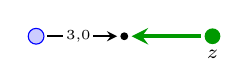
\begin{tikzpicture}[scale=0.35, baseline=0cm]
	\node at (0.9,0.2)  [root] (root) {};
	\node at (0.9,0.2) [rootlab] {$z$};
	\node at (-2.3, 0.2)  [dot] (int) {};
	\node at (-5.5,0.2)  [var_blue] (left) {};	
	\draw[testfcn] (int) to (root);	
	\draw[keps] (left) to node[labl,pos=0.45] {\tiny 3,0} (int);
\end{tikzpicture}\;.
\end{equation*}
This diagram is the stochastic integral $\CI^{\eps} (F)$, where the kernel $F$ is in this case the generalised convolution $\CK^{\lambda, \eps}_{\CCG, z}$, as in \eqref{e:genconv_shift}, given by
\begin{equation*}
\CK^{\lambda, \eps}_{\CCG, z}(z^{\var}) = \int_{D_\eps} \!\!\phi_z^\lambda(\bar z)\, K^{\epsEH}(\bar z - z^{\var})\, \d \bar z.
\end{equation*}
One can check that Assumption~\ref{a:mainContraction} is satisfied for this diagram with a trivial contraction: from the diagram we see that $| \hat \CCV_{\!\var}| = 1$ and $|\hat \CCV_{\!\bar\star} \setminus \{ v^\uparrow_{\!\star} \}| = 1$. The space-time scaling is $\s = (2, 1, 1, 1)$, so that $|\s|=5$ and the value of the constant $\nu_\gamma$ in \eqref{e:genconvBound} is $-\frac{1}{2}$. Applying Corollary~\ref{cor:convolutions} with $\Gamma = \{ 1 \}$ and recalling that $|\tau| = -\frac{1}{2}-\kappa$, one obtains the bound 
\begin{equation*}
\Bigl( \E \bigl| \iota_\eps ( \hat \Pi^\eps_z \tau)(\phi^\lambda_z)\bigr|^p\Bigr)^{\frac{1}{p}} \lesssim (\lambda \vee \epsEH)^{- \frac{1}{2}} \big( 1 + \eps^{\frac52 - \bar{k}} \epsEH^{-\frac52} \big).
\end{equation*}
As such, we immediately get \eqref{e:model_bound} for the element $\tau$.

In what follows, we prefer not to specify contractions $\gamma$ every time, as it will be clear from diagrams. 

\subsection{The element $\tau = \Psi^2$}
\label{sec:symbol-3}

Taking into account the renormalisation in \eqref{eq:Pi-and-Psi2}, the map $\hat \Pi_{z}^{\eps}\tau$ can be represented by the diagrams
\begin{equation}\label{e:Pi2}
	\iota_\eps (\hat \Pi_{z}^{\eps}\tau)(\phi_z^\lambda)
	\;=\; 
	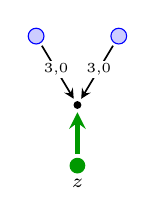
\begin{tikzpicture}[scale=0.35, baseline=0cm]
		\node at (0,-2.2)  [root] (root) {};
		\node at (0,-2.2) [rootlab] {$z$};
		\node at (0,-2.5) {$$};
		\node at (0,0)  [dot] (int) {};
		\node at (-1.5,2.5)  [var_blue] (left) {};
		\node at (1.5,2.5)  [var_blue] (right) {};
		
		\draw[testfcn] (int) to (root);
		
		\draw[keps] (left) to node[labl,pos=0.45] {\tiny 3,0} (int);
		\draw[keps] (right) to node[labl,pos=0.45] {\tiny 3,0} (int);
	\end{tikzpicture}
	\; +\;
	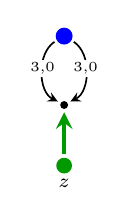
\begin{tikzpicture}[scale=0.35, baseline=0cm]
		\node at (0,-2.2)  [root] (root) {};
		\node at (0,-2.2) [rootlab] {$z$};
		\node at (0,0)  [dot] (int) {};
		\node at (0,2.5)  [var_very_blue] (left) {};
		
		\draw[testfcn] (int) to (root);
		
		\draw[keps] (left) to[bend left=60] node[labl,pos=0.45] {\tiny 3,0} (int);
		\draw[keps] (left) to[bend left=-60] node[labl,pos=0.45] {\tiny 3,0} (int);
	\end{tikzpicture}
	\; -\; C^\eps_1\, 
	
\begin{tikzpicture}[scale=0.35, baseline=-0.5cm]
		\node at (0,-2.2)  [root] (root) {};
		\node at (0,-2.2) [rootlab] {$z$};
		\node at (0,0)  [dot] (int) {};
		
		\draw[testfcn] (int) to (root);
	\end{tikzpicture}\;.
\end{equation}
where the renormalisation constant is given in \eqref{e:Phi_C1}. Let us denote by ``\,\tikz[baseline=-3] \node [var_red_square] {};\,'' the variable which is integrated with respect to the martingales $t \mapsto ( [ \M_\eps(x) ]_t - \langle \M_\eps(x) \rangle_t )_{x \in \Le}$. Then, by \eqref{eq:RenormIntegrals}, our choice of the renormalisation constant allows to write \eqref{e:Pi2} as 
\begin{equation}\label{e:Pi2-new}
\iota_\eps (\hat \Pi_{z}^{\eps}\tau)(\phi_z^\lambda)
\;=\; 
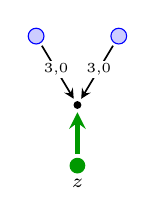
\begin{tikzpicture}[scale=0.35, baseline=0cm]
	\node at (0,-2.2)  [root] (root) {};
	\node at (0,-2.2) [rootlab] {$z$};
	\node at (0,-2.5) {$$};
	\node at (0,0)  [dot] (int) {};
	\node at (-1.5,2.5)  [var_blue] (left) {};
	\node at (1.5,2.5)  [var_blue] (right) {};
	
	\draw[testfcn] (int) to (root);
	
	\draw[keps] (left) to node[labl,pos=0.45] {\tiny 3,0} (int);
	\draw[keps] (right) to node[labl,pos=0.45] {\tiny 3,0} (int);
\end{tikzpicture}
\; +\;
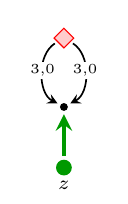
\begin{tikzpicture}[scale=0.35, baseline=0cm]
	\node at (0,-2.2)  [root] (root) {};
	\node at (0,-2.2) [rootlab] {$z$};
	\node at (0,0)  [dot] (int) {};
	\node at (0,2.5)  [var_red_square] (left) {};
	
	\draw[testfcn] (int) to (root);
	
	\draw[keps] (left) to[bend left=60] node[labl,pos=0.45] {\tiny 3,0} (int);
	\draw[keps] (left) to[bend left=-60] node[labl,pos=0.45] {\tiny 3,0} (int);
\end{tikzpicture},
\end{equation}
Let us denote these two diagrams by $\iota_\eps (\hat \Pi_{z}^{\eps, 1}\tau)(\phi_z^\lambda)$ and $\iota_\eps (\hat \Pi_{z}^{\eps, 2}\tau)(\phi_z^\lambda)$ respectively.

Let us start with the first diagram in \eqref{e:Pi2-new}. Assumption~\ref{a:mainContraction} is satisfied for it with a trivial contraction, and the bound \eqref{e:genconvBound} holds with the set $\Gamma = \{1, 2\}$. Furthermore, we have $| \hat \CCV_{\!\var}| = 2$ and $|\hat \CCV_{\!\bar\star} \setminus \{ v^\uparrow_{\!\star} \}| = 2$ and the value of the constant $\nu_\gamma$ in \eqref{e:genconvBound} is $-1$. Applying Corollary~\ref{cor:convolutions} to this diagram, we get the bound 
\begin{equation*}
 \Bigl(\E \bigl| \iota_\eps( \hat \Pi^{\eps, 1}_z \tau)(\phi^\lambda_z)\bigr|^p\Bigr)^{\frac{1}{p}} \lesssim (\lambda \vee \epsEH)^{-1} \bigl(1 + \eps^{\frac52 - \bar{k}} \epsEH^{-\frac52} + \eps^{5 - \bar{k}} \epsEH^{-5}\bigr).
\end{equation*}
Recalling that $|\tau| = -1-2\kappa$ and that $\eps$ is smaller than $\epsEH$, we get the bound \eqref{e:model_bound}.

The second diagram in \eqref{e:Pi2-new} does not satisfy Assumption~\ref{a:mainContraction}, because the kernels have very strong singularities. To solve this problem, we notice that multiplication of a kernel by a positive power of $\eps$ decreases the order of singularity in \eqref{eq:K_bound}. Hence, for any $0 < a < 3$ we can write the last diagram in \eqref{e:Pi2-new} as
\begin{equation}\label{eq:cherry-contracted} \eps^{2 (a - 3)}
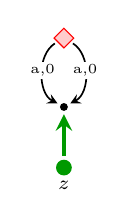
\begin{tikzpicture}[scale=0.35, baseline=0cm]
	\node at (0,-2.2)  [root] (root) {};
	\node at (0,-2.2) [rootlab] {$z$};
	\node at (0,-2.5) {$$};
	\node at (0,0)  [dot] (int) {};
	\node at (0,2.5)  [var_red_square] (left) {};
	
	\draw[testfcn] (int) to (root);
	
	\draw[keps] (left) to[bend left=60] node[labl,pos=0.45] {\tiny a,0} (int);
	\draw[keps] (left) to[bend left=-60] node[labl,pos=0.45] {\tiny a,0} (int);
\end{tikzpicture},
\end{equation}
where we multiplied each kernel by $\eps^{3-a}$. For $a < \frac{5}{2}$ Assumption~\ref{a:mainContraction} is satisfied and Corollary~\ref{cor:convolutions} yields 
\begin{equation*}
	\Bigl(\E \bigl|\iota_\eps( \hat \Pi^{\eps, 2}_z \tau)(\phi^\lambda_z)\bigr|^p\Bigr)^{\frac{1}{p}} \lesssim \eps^{2a - 6} (\lambda \vee \epsEH)^{\frac52 - 2a} \big( \eps^{\frac52} + \eps^{5 - \bar k} \epsEH^{\frac52} \big) \lesssim \eps^{2a - \frac72} .
\end{equation*}
If we choose $a > \frac74$, then this term disappears in the limit. Notice that here the only difference with the case $\tau = \Psi$ is that the coefficient $\alpha_\ga(A, B)$ coming from Corollary~\ref{cor:convolutions} is larger.

\subsection{The element $\tau = \CI(\Psi^3) \Psi^2$} 
\label{sec:last_symbol}

Using the definition \eqref{eq:Pi-and-last}, the diagrams for the map $\hat \Pi_{z}^{\eps}\tau$ are the following:
\begin{align} \nonumber
\iota_\eps &(\hat \Pi_{z}^{\eps}\tau)(\phi_z^\lambda)
\;=\; 
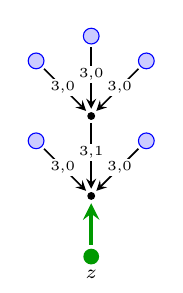
\begin{tikzpicture}[scale=0.35, baseline=-0.5cm]
	\node at (0,-5.1)  [root] (root) {};
	\node at (0,-5.1) [rootlab] {$z$};
	\node at (0,0) [dot] (int) {};
	\node at (-2,2) [var_blue] (left) {};
	\node at (0,2.9)  [var_blue] (cent) {};
	\node at (2,2)  [var_blue] (right) {};
	\node at (0,-2.9) [dot] (cent1) {};
	\node at (2,-0.9)  [var_blue] (right1) {};
	\node at (-2,-0.9)  [var_blue] (left1) {};
	\draw[testfcn] (cent1) to (root);
	\draw[keps] (left) to node[labl,pos=0.45] {\tiny 3,0} (int);
	\draw[keps] (right) to node[labl,pos=0.45] {\tiny 3,0} (int);
	\draw[keps] (cent) to node[labl,pos=0.45] {\tiny 3,0} (int);
	\draw[keps] (int) to node[labl,pos=0.45] {\tiny 3,1} (cent1);
	\draw[keps] (right1) to node[labl,pos=0.45] {\tiny 3,0} (cent1);
	\draw[keps] (left1) to node[labl,pos=0.45] {\tiny 3,0} (cent1);
\end{tikzpicture}
\; +\;3\,
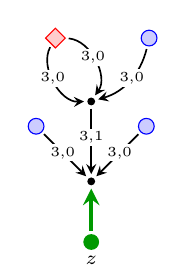
\begin{tikzpicture}[scale=0.35, baseline=-0.5cm]
	\node at (0,-5.1)  [root] (root) {};
	\node at (0,-5.1) [rootlab] {$z$};
	\node at (0,0)  [dot] (int) {};
	\node at (-1.3,2.3)  [var_red_square] (left) {};
	\node at (2.1,2.3)  [var_blue] (right) {};
	\node at (0,-2.9) [dot] (cent1) {};
	\node at (2,-0.9)  [var_blue] (right1) {};
	\node at (-2,-0.9)  [var_blue] (left1) {};
	\draw[testfcn] (cent1) to (root);
	\draw[keps] (left) to[bend left=60] node[labl,pos=0.45] {\tiny 3,0} (int);
	\draw[keps] (left) to[bend left=-60] node[labl,pos=0.45] {\tiny 3,0} (int);
	\draw[keps] (right) to[bend left=30] node[labl,pos=0.45] {\tiny 3,0} (int);
	\draw[keps] (int) to node[labl,pos=0.45] {\tiny 3,1} (cent1);
	\draw[keps] (right1) to node[labl,pos=0.45] {\tiny 3,0} (cent1);
	\draw[keps] (left1) to node[labl,pos=0.45] {\tiny 3,0} (cent1);
\end{tikzpicture}
\; +\;
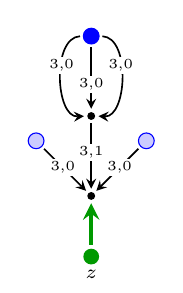
\begin{tikzpicture}[scale=0.35, baseline=-0.5cm]
	\node at (0,-5.1)  [root] (root) {};
	\node at (0,-5.1) [rootlab] {$z$};
	\node at (0,0)  [dot] (int) {};
	\node at (0,2.9)  [var_very_blue] (left) {};
	\node at (0,-2.9) [dot] (cent1) {};
	\node at (2,-0.9)  [var_blue] (right1) {};
	\node at (-2,-0.9)  [var_blue] (left1) {};
	\draw[testfcn] (cent1) to (root);
	\draw[keps] (left) to[bend left=90] node[labl,pos=0.4] {\tiny 3,0} (int);
	\draw[keps] (left) to[bend left=-90] node[labl,pos=0.4] {\tiny 3,0} (int);
	\draw[keps] (left) to node[labl,pos=0.6] {\tiny 3,0} (int);
	\draw[keps] (int) to node[labl,pos=0.45] {\tiny 3,1} (cent1);
	\draw[keps] (right1) to node[labl,pos=0.45] {\tiny 3,0} (cent1);
	\draw[keps] (left1) to node[labl,pos=0.45] {\tiny 3,0} (cent1);
\end{tikzpicture}
\; +\;
2\,
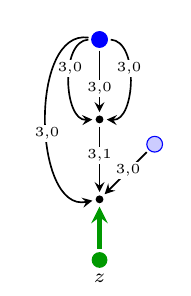
\begin{tikzpicture}[scale=0.35, baseline=-0.5cm]
	\node at (0,-5.1)  [root] (root) {};
	\node at (0,-5.1) [rootlab] {$z$};
	\node at (0,0)  [dot] (int) {};
	\node at (0,2.9)  [var_very_blue] (left) {};
	\node at (0,-2.9) [dot] (cent1) {};
	\node at (2,-0.9)  [var_blue] (right1) {};
	\draw[testfcn] (cent1) to (root);
	\draw[keps] (left) to[bend left=90] node[labl,pos=0.4] {\tiny 3,0} (int);
	\draw[keps] (left) to[bend left=-90] node[labl,pos=0.4] {\tiny 3,0} (int);
	\draw[keps] (left) to node[labl,pos=0.6] {\tiny 3,0} (int);
	\draw[keps] (int) to node[labl,pos=0.45] {\tiny 3,1} (cent1);
	\draw[keps] (left) to[bend right=100] node[labl,pos=0.55] {\tiny 3,0} (cent1);
	\draw[keps] (right1) to node[labl,pos=0.45] {\tiny 3,0} (cent1);
\end{tikzpicture}
\; +\;3\,
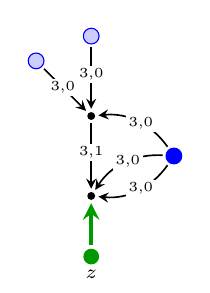
\begin{tikzpicture}[scale=0.35, baseline=-0.5cm]
	\node at (0,-5.1)  [root] (root) {};
	\node at (0,-5.1) [rootlab] {$z$};
	\node at (0,-4.5) {$$};
	\node at (0,0) [dot] (int) {};
	\node at (-2,2) [var_blue] (left) {};
	\node at (0,2.9)  [var_blue] (cent) {};
	\node at (0,-2.9) [dot] (cent1) {};
	\node at (3,-1.45)  [var_very_blue] (right1) {};
	\draw[testfcn] (cent1) to (root);
	\draw[keps] (left) to node[labl,pos=0.45] {\tiny 3,0} (int);
	\draw[keps] (right1) to[bend left=-30] node[labl,pos=0.45] {\tiny 3,0} (int);
	\draw[keps] (cent) to node[labl,pos=0.45] {\tiny 3,0} (int);
	\draw[keps] (int) to node[labl,pos=0.45] {\tiny 3,1} (cent1);
	\draw[keps] (right1) to[bend left=-30] node[labl,pos=0.45] {\tiny 3,0} (cent1);
	\draw[keps] (right1) to[bend left=30] node[labl,pos=0.45] {\tiny 3,0} (cent1);
\end{tikzpicture}\\[0.5cm]
&\label{eq:last-tree}
\; +\;6\,
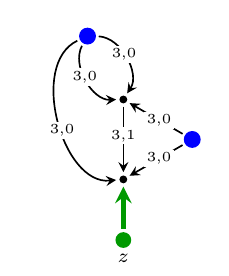
\begin{tikzpicture}[scale=0.35, baseline=-0.5cm]
	\node at (0,-5.1)  [root] (root) {};
	\node at (0,-5.1) [rootlab] {$z$};
	\node at (0,0)  [dot] (int) {};
	\node at (-1.3,2.3)  [var_very_blue] (left) {};
	\node at (0,-2.9) [dot] (cent1) {};
	\node at (2.5,-1.45)  [var_very_blue] (right1) {};
	\draw[testfcn] (cent1) to (root);
	\draw[keps] (left) to[bend left=60] node[labl,pos=0.45] {\tiny 3,0} (int);
	\draw[keps] (left) to[bend left=-60] node[labl,pos=0.45] {\tiny 3,0} (int);
	\draw[keps] (right1) to node[labl,pos=0.45] {\tiny 3,0} (int);
	\draw[keps] (int) to node[labl,pos=0.45] {\tiny 3,1} (cent1);
	\draw[keps] (right1) to node[labl,pos=0.45] {\tiny 3,0} (cent1);
	\draw[keps] (left) to[bend left=-80] node[labl,pos=0.55] {\tiny 3,0} (cent1);
\end{tikzpicture}
\; +\;3\,
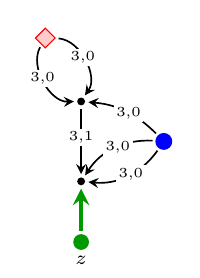
\begin{tikzpicture}[scale=0.35, baseline=-0.5cm]
	\node at (0,-5.1)  [root] (root) {};
	\node at (0,-5.1) [rootlab] {$z$};
	\node at (0,0)  [dot] (int) {};
	\node at (-1.3,2.3)  [var_red_square] (left) {};
	\node at (0,-2.9) [dot] (cent1) {};
	\node at (3,-1.45) [var_very_blue] (right1) {};
	\draw[testfcn] (cent1) to (root);
	\draw[keps] (left) to[bend left=60] node[labl,pos=0.45] {\tiny 3,0} (int);
	\draw[keps] (left) to[bend left=-60] node[labl,pos=0.45] {\tiny 3,0} (int);
	\draw[keps] (right1) to[bend left=-20] node[labl,pos=0.45] {\tiny 3,0} (int);
	\draw[keps] (int) to node[labl,pos=0.45] {\tiny 3,1} (cent1);
	\draw[keps] (right1) to[bend left=-30] node[labl,pos=0.45] {\tiny 3,0} (cent1);
	\draw[keps] (right1) to[bend left=30] node[labl,pos=0.45] {\tiny 3,0} (cent1);
\end{tikzpicture}
\;+\;6\,
\begin{tikzpicture}[scale=0.35, baseline=-0.5cm]
	\node at (0,-5.1)  [root] (root) {};
	\node at (0,-5.1) [rootlab] {$z$};
	\node at (0,0)  [dot] (int) {};
	\node at (2.5,-1.45)  [var_very_blue] (right1) {};
	\node at (-2,-0.9)  [var_blue] (left1) {};
	\node at (-2,2) [var_blue] (left) {};
	\node at (0,2.9)  [var_blue] (cent) {};
	\draw[testfcn] (cent1) to (root);
	\draw[keps] (left) to node[labl,pos=0.45] {\tiny 3,0} (int);
	\draw[keps] (cent) to node[labl,pos=0.45] {\tiny 3,0} (int);
	\draw[keps] (right1) to node[labl,pos=0.45] {\tiny 3,0} (int);
	\draw[keps] (int) to node[labl,pos=0.45] {\tiny 3,1} (cent1);
	\draw[keps] (right1) to node[labl,pos=0.45] {\tiny 3,0} (cent1);
	\draw[keps] (left1) to node[labl,pos=0.45] {\tiny 3,0} (cent1);
\end{tikzpicture}
\; +\;6\,
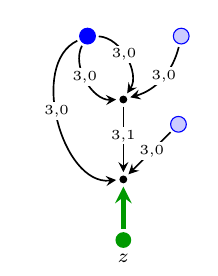
\begin{tikzpicture}[scale=0.35, baseline=-0.5cm]
	\node at (0,-5.1)  [root] (root) {};
	\node at (0,-5.1) [rootlab] {$z$};
	\node at (0,0)  [dot] (int) {};
	\node at (-1.3,2.3)  [var_very_blue] (left) {};
	\node at (2.1,2.3)  [var_blue] (right) {};
	\node at (0,-2.9) [dot] (cent1) {};
	\node at (2,-0.9)  [var_blue] (right1) {};
	\draw[testfcn] (cent1) to (root);s
	\draw[keps] (left) to[bend left=60] node[labl,pos=0.45] {\tiny 3,0} (int);
	\draw[keps] (left) to[bend left=-60] node[labl,pos=0.45] {\tiny 3,0} (int);
	\draw[keps] (right) to[bend left=30] node[labl,pos=0.45] {\tiny 3,0} (int);
	\draw[keps] (int) to node[labl,pos=0.45] {\tiny 3,1} (cent1);
	\draw[keps] (left) to[bend left=-80] node[labl,pos=0.45] {\tiny 3,0} (cent1);
	\draw[keps] (right1) to node[labl,pos=0.45] {\tiny 3,0} (cent1);
\end{tikzpicture}
\; +\;
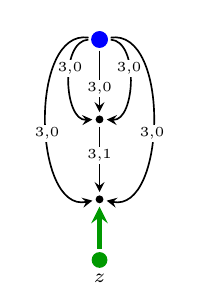
\begin{tikzpicture}[scale=0.35, baseline=-0.5cm]
	\node at (0,-5.1)  [root] (root) {};
	\node at (0,-5.1) [rootlab] {$z$};
	\node at (0,0)  [dot] (int) {};
	\node at (0,2.9)  [var_very_blue] (left) {};
	\node at (0,-2.9) [dot] (cent1) {};
	\draw[testfcn] (cent1) to (root);
	\draw[keps] (left) to[bend left=90] node[labl,pos=0.4] {\tiny 3,0} (int);
	\draw[keps] (left) to[bend left=-90] node[labl,pos=0.4] {\tiny 3,0} (int);
	\draw[keps] (left) to node[labl,pos=0.6] {\tiny 3,0} (int);
	\draw[keps] (int) to node[labl,pos=0.45] {\tiny 3,1} (cent1);
	\draw[keps] (left) to[bend left=100] node[labl,pos=0.55] {\tiny 3,0} (cent1);
	\draw[keps] (left) to[bend right=100] node[labl,pos=0.55] {\tiny 3,0} (cent1);
\end{tikzpicture}\\[0.5cm]
&\; +\;3\,
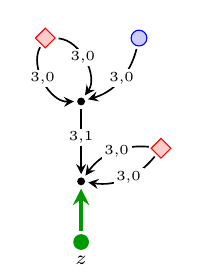
\begin{tikzpicture}[scale=0.35, baseline=-0.5cm]
	\node at (0,-5.1)  [root] (root) {};
	\node at (0,-5.1) [rootlab] {$z$};
	\node at (0,0)  [dot] (int) {};
	\node at (-1.3,2.3)  [var_red_square] (left) {};
	\node at (2.1,2.3)  [var_blue] (right) {};
	\node at (0,-2.9) [dot] (cent1) {};
	\node at (2.9,-1.7) [var_red_square] (right1) {};
	\draw[testfcn] (cent1) to (root);
	\draw[keps] (left) to[bend left=60] node[labl,pos=0.45] {\tiny 3,0} (int);
	\draw[keps] (left) to[bend left=-60] node[labl,pos=0.45] {\tiny 3,0} (int);
	\draw[keps] (int) to node[labl,pos=0.45] {\tiny 3,1} (cent1);
	\draw[keps] (right1) to[bend left=-30] node[labl,pos=0.45] {\tiny 3,0} (cent1);
	\draw[keps] (right1) to[bend left=30] node[labl,pos=0.45] {\tiny 3,0} (cent1);
	\draw[keps] (right) to[bend left=30] node[labl,pos=0.45] {\tiny 3,0} (int);
\end{tikzpicture}
\; +\;6\,
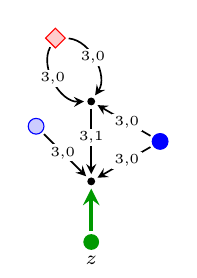
\begin{tikzpicture}[scale=0.35, baseline=-0.5cm]
	\node at (0,-5.1)  [root] (root) {};
	\node at (0,-5.1) [rootlab] {$z$};
	\node at (0,0)  [dot] (int) {};
	\node at (-1.3,2.3)  [var_red_square] (left) {};
	\node at (0,-2.9) [dot] (cent1) {};
	\node at (2.5,-1.45)  [var_very_blue] (right1) {};
	\node at (-2,-0.9)  [var_blue] (left1) {};
	\draw[testfcn] (cent1) to (root);
	\draw[keps] (left) to[bend left=60] node[labl,pos=0.45] {\tiny 3,0} (int);
	\draw[keps] (left) to[bend left=-60] node[labl,pos=0.45] {\tiny 3,0} (int);
	\draw[keps] (right1) to node[labl,pos=0.45] {\tiny 3,0} (int);
	\draw[keps] (int) to node[labl,pos=0.45] {\tiny 3,1} (cent1);
	\draw[keps] (right1) to node[labl,pos=0.45] {\tiny 3,0} (cent1);
	\draw[keps] (left1) to node[labl,pos=0.45] {\tiny 3,0} (cent1);
\end{tikzpicture}
\;+\;
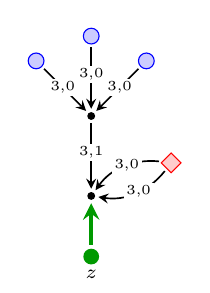
\begin{tikzpicture}[scale=0.35, baseline=-0.5cm]
	\node at (0,-5.1)  [root] (root) {};
	\node at (0,-5.1) [rootlab] {$z$};
	\node at (0,0) [dot] (int) {};
	\node at (-2,2) [var_blue] (left) {};
	\node at (0,2.9) [var_blue] (cent) {};
	\node at (2,2) [var_blue] (right) {};
	\node at (0,-2.9) [dot] (cent1) {};
	\node at (2.9,-1.7) [var_red_square] (right1) {};
	\draw[testfcn] (cent1) to (root);
	\draw[keps] (left) to node[labl,pos=0.45] {\tiny 3,0} (int);
	\draw[keps] (right) to node[labl,pos=0.45] {\tiny 3,0} (int);
	\draw[keps] (cent) to node[labl,pos=0.45] {\tiny 3,0} (int);
	\draw[keps] (int) to node[labl,pos=0.45] {\tiny 3,1} (cent1);
	\draw[keps] (right1) to[bend left=-30] node[labl,pos=0.45] {\tiny 3,0} (cent1);
	\draw[keps] (right1) to[bend left=30] node[labl,pos=0.45] {\tiny 3,0} (cent1);
\end{tikzpicture}
\; +\;
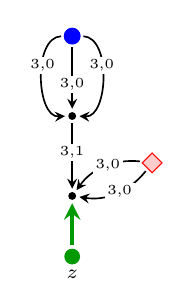
\begin{tikzpicture}[scale=0.35, baseline=-0.5cm]
	\node at (0,-5.1)  [root] (root) {};
	\node at (0,-5.1) [rootlab] {$z$};
	\node at (0,0)  [dot] (int) {};
	\node at (0,2.9)  [var_very_blue] (left) {};
	\node at (0,-2.9) [dot] (cent1) {};
	\node at (2.9,-1.7) [var_red_square] (right1) {};
	\draw[testfcn] (cent1) to (root);
	\draw[keps] (left) to[bend left=90] node[labl,pos=0.4] {\tiny 3,0} (int);
	\draw[keps] (left) to[bend left=-90] node[labl,pos=0.4] {\tiny 3,0} (int);
	\draw[keps] (left) to node[labl,pos=0.6] {\tiny 3,0} (int);
	\draw[keps] (int) to node[labl,pos=0.45] {\tiny 3,1} (cent1);
	\draw[keps] (right1) to[bend left=-30] node[labl,pos=0.45] {\tiny 3,0} (cent1);
	\draw[keps] (right1) to[bend left=30] node[labl,pos=0.45] {\tiny 3,0} (cent1);
\end{tikzpicture} + \\[0.5cm]
& \; +\; 6\;
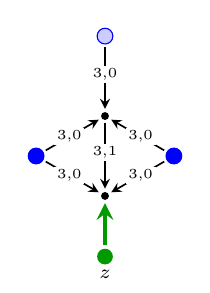
\begin{tikzpicture}[scale=0.35, baseline=-0.5cm]
	\node at (0,-5.1)  [root] (root) {};
	\node at (0,-5.1) [rootlab] {$z$};
	\node at (0,0) [dot] (int) {};
	\node at (0,2.9)  [var_blue] (cent) {};
	\node at (0,-2.9) [dot] (cent1) {};
	\node at (2.5,-1.45)  [var_very_blue] (right1) {};
	\node at (-2.5,-1.45)  [var_very_blue] (left1) {};
	\draw[testfcn] (cent1) to (root);
	\draw[keps] (left1) to node[labl,pos=0.45] {\tiny 3,0} (int);
	\draw[keps] (right1) to node[labl,pos=0.45] {\tiny 3,0} (int);
	\draw[keps] (cent) to node[labl,pos=0.45] {\tiny 3,0} (int);
	\draw[keps] (int) to node[labl,pos=0.45] {\tiny 3,1} (cent1);
	\draw[keps] (right1) to node[labl,pos=0.45] {\tiny 3,0} (cent1);
	\draw[keps] (left1) to node[labl,pos=0.45] {\tiny 3,0} (cent1);
\end{tikzpicture}
\; -\;3 C^\eps_2\;
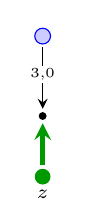
\begin{tikzpicture}[scale=0.35, baseline=-0.7cm]
	\node at (0,-5.1)  [root] (root) {};
	\node at (0,-5.1) [rootlab] {$z$};
	\node at (0,0)  [var_blue] (cent) {};
	\node at (0,-2.9) [dot] (cent1) {};
	\draw[testfcn] (cent1) to (root);
	\draw[keps] (cent) to node[labl,pos=0.45] {\tiny 3,0} (cent1);
\end{tikzpicture}\;. \nonumber
\end{align}
All these diagrams, except the tenth and the last two, can be bounded by a direct application of Corollary~\ref{cor:convolutions}.

To bound the tenth diagram (the one that contracts all leaves), we write
\begin{equation*}
	\bM^{\otimes 5}_\eps ( A_\ga) = \eps^{15} \sum_{x \in \Le} \sum_{0 \leq s \leq T} \big(\Delta_s \M_{\eps}(x) \big)^{5} = \eps^{13} \sum_{x \in \Le} \sum_{0 \leq s \leq T} \Delta_s \M_{\eps}(x),
\end{equation*}
where $\gamma \in \fC_1(\CCV_{\!\var})$ and $|\CCV_{\!\var}| = |\gamma_1| = 5$. Then we can write 
\begin{equation*}
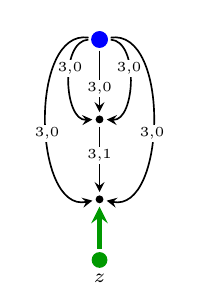
\begin{tikzpicture}[scale=0.35, baseline=-0.5cm]
	\node at (0,-5.1)  [root] (root) {};
	\node at (0,-5.1) [rootlab] {$z$};
	\node at (0,0)  [dot] (int) {};
	\node at (0,2.9)  [var_very_blue] (left) {};
	\node at (0,-2.9) [dot] (cent1) {};
	\draw[testfcn] (cent1) to (root);
	\draw[keps] (left) to[bend left=90] node[labl,pos=0.4] {\tiny 3,0} (int);
	\draw[keps] (left) to[bend left=-90] node[labl,pos=0.4] {\tiny 3,0} (int);
	\draw[keps] (left) to node[labl,pos=0.6] {\tiny 3,0} (int);
	\draw[keps] (int) to node[labl,pos=0.45] {\tiny 3,1} (cent1);
	\draw[keps] (left) to[bend left=100] node[labl,pos=0.55] {\tiny 3,0} (cent1);
	\draw[keps] (left) to[bend right=100] node[labl,pos=0.55] {\tiny 3,0} (cent1);
\end{tikzpicture}
\;=\; \eps^{10}
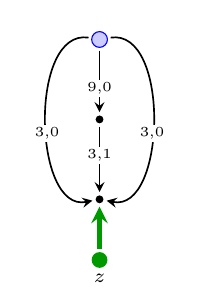
\begin{tikzpicture}[scale=0.35, baseline=-0.5cm]
	\node at (0,-5.1)  [root] (root) {};
	\node at (0,-5.1) [rootlab] {$z$};
	\node at (0,0)  [dot] (int) {};
	\node at (0,2.9)  [var_blue] (left) {};
	\node at (0,-2.9) [dot] (cent1) {};
	\draw[testfcn] (cent1) to (root);
	\draw[keps] (left) to node[labl,pos=0.6] {\tiny 9,0} (int);
	\draw[keps] (int) to node[labl,pos=0.45] {\tiny 3,1} (cent1);
	\draw[keps] (left) to[bend left=100] node[labl,pos=0.55] {\tiny 3,0} (cent1);
	\draw[keps] (left) to[bend right=100] node[labl,pos=0.55] {\tiny 3,0} (cent1);
\end{tikzpicture},
\end{equation*}
where the stochastic integral is with respect to the martingale $\M_{\eps}$. Taking powers of $\eps$ to improve the singularities of the kernels, Corollary~\ref{cor:convolutions} allows to bound moments of this diagram by $(\lambda \vee \epsEH)^{|\tau|}$, and the remaining positive $\eps$ power makes it vanish in the limit. 
\medskip

We now turn our attention to the last two diagrams in \eqref{eq:last-tree}, which are also the most interesting ones. We can write
\begin{align} \label{eq:important_subtree}
	2\;
	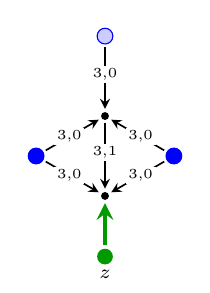
\begin{tikzpicture}[scale=0.35, baseline=-0.5cm]
		\node at (0,-5.1)  [root] (root) {};
		\node at (0,-5.1) [rootlab] {$z$};
		\node at (0,0) [dot] (int) {};
		\node at (0,2.9)  [var_blue] (cent) {};
		\node at (0,-2.9) [dot] (cent1) {};
		\node at (2.5,-1.45)  [var_very_blue] (right1) {};
		\node at (-2.5,-1.45)  [var_very_blue] (left1) {};
		\draw[testfcn] (cent1) to (root);
		\draw[keps] (left1) to node[labl,pos=0.45] {\tiny 3,0} (int);
		\draw[keps] (right1) to node[labl,pos=0.45] {\tiny 3,0} (int);
		\draw[keps] (cent) to node[labl,pos=0.45] {\tiny 3,0} (int);
		\draw[keps] (int) to node[labl,pos=0.45] {\tiny 3,1} (cent1);
		\draw[keps] (right1) to node[labl,pos=0.45] {\tiny 3,0} (cent1);
		\draw[keps] (left1) to node[labl,pos=0.45] {\tiny 3,0} (cent1);
	\end{tikzpicture}
	\; -\; C^\eps_2 \;
	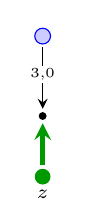
\begin{tikzpicture}[scale=0.35, baseline=-0.7cm]
		\node at (0,-5.1)  [root] (root) {};
		\node at (0,-5.1) [rootlab] {$z$};
		\node at (0,0)  [var_blue] (cent) {};
		\node at (0,-2.9) [dot] (cent1) {};
		\draw[testfcn] (cent1) to (root);
		\draw[keps] (cent) to node[labl,pos=0.45] {\tiny 3,0} (cent1);
	\end{tikzpicture}
	\; = \; \left(
	2\;
	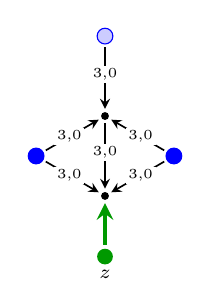
\begin{tikzpicture}[scale=0.35, baseline=-0.5cm]
		\node at (0,-5.1)  [root] (root) {};
		\node at (0,-5.1) [rootlab] {$z$};
		\node at (0,0) [dot] (int) {};
		\node at (0,2.9)  [var_blue] (cent) {};
		\node at (0,-2.9) [dot] (cent1) {};
		\node at (2.5,-1.45)  [var_very_blue] (right1) {};
		\node at (-2.5,-1.45)  [var_very_blue] (left1) {};
		\draw[testfcn] (cent1) to (root);
		\draw[keps] (left1) to node[labl,pos=0.45] {\tiny 3,0} (int);
		\draw[keps] (right1) to node[labl,pos=0.45] {\tiny 3,0} (int);
		\draw[keps] (cent) to node[labl,pos=0.45] {\tiny 3,0} (int);
		\draw[keps] (int) to node[labl,pos=0.45] {\tiny 3,0} (cent1);
		\draw[keps] (right1) to node[labl,pos=0.45] {\tiny 3,0} (cent1);
		\draw[keps] (left1) to node[labl,pos=0.45] {\tiny 3,0} (cent1);
	\end{tikzpicture}
	\; -\; C^\eps_2 \;
	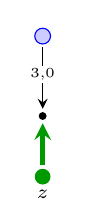
\begin{tikzpicture}[scale=0.35, baseline=-0.7cm]
		\node at (0,-5.1)  [root] (root) {};
		\node at (0,-5.1) [rootlab] {$z$};
		\node at (0,0)  [var_blue] (cent) {};
		\node at (0,-2.9) [dot] (cent1) {};
		\draw[testfcn] (cent1) to (root);
		\draw[keps] (cent) to node[labl,pos=0.45] {\tiny 3,0} (cent1);
	\end{tikzpicture} \right)
	\; -\; 2\;
	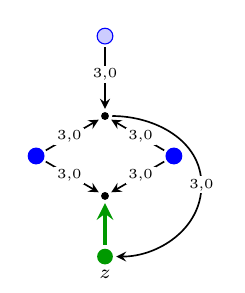
\begin{tikzpicture}[scale=0.35, baseline=-0.5cm]
		\node at (0,-5.1)  [root] (root) {};
		\node at (0,-5.1) [rootlab] {$z$};
		\node at (0,0) [dot] (int) {};
		\node at (0,2.9)  [var_blue] (cent) {};
		\node at (0,-2.9) [dot] (cent1) {};
		\node at (2.5,-1.45)  [var_very_blue] (right1) {};
		\node at (-2.5,-1.45)  [var_very_blue] (left1) {};
		\draw[testfcn] (cent1) to (root);
		\draw[keps] (left1) to node[labl,pos=0.45] {\tiny 3,0} (int);
		\draw[keps] (right1) to node[labl,pos=0.45] {\tiny 3,0} (int);
		\draw[keps] (cent) to node[labl,pos=0.45] {\tiny 3,0} (int);
		\draw[keps] (right1) to node[labl,pos=0.45] {\tiny 3,0} (cent1);
		\draw[keps] (left1) to node[labl,pos=0.45] {\tiny 3,0} (cent1);
		\draw [keps] (int) to[out=0,in=90] (3.5,-2.5) to [out=-90, in=0] node[labl,pos=0] {\tiny 3,0} (root);
	\end{tikzpicture}\;.
\end{align}
The last diagram can be first decomposed as 
\[
	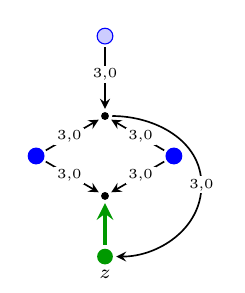
\begin{tikzpicture}[scale=0.35, baseline=-0.5cm]
		\node at (0,-5.1)  [root] (root) {};
		\node at (0,-5.1) [rootlab] {$z$};
		\node at (0,0) [dot] (int) {};
		\node at (0,2.9)  [var_blue] (cent) {};
		\node at (0,-2.9) [dot] (cent1) {};
		\node at (2.5,-1.45)  [var_very_blue] (right1) {};
		\node at (-2.5,-1.45)  [var_very_blue] (left1) {};
		\draw[testfcn] (cent1) to (root);
		\draw[keps] (left1) to node[labl,pos=0.45] {\tiny 3,0} (int);
		\draw[keps] (right1) to node[labl,pos=0.45] {\tiny 3,0} (int);
		\draw[keps] (cent) to node[labl,pos=0.45] {\tiny 3,0} (int);
		\draw[keps] (right1) to node[labl,pos=0.45] {\tiny 3,0} (cent1);
		\draw[keps] (left1) to node[labl,pos=0.45] {\tiny 3,0} (cent1);
		\draw [keps] (int) to[out=0,in=90] (3.5,-2.5) to [out=-90, in=0] node[labl,pos=0] {\tiny 3,0} (root);
	\end{tikzpicture}\;
	=
	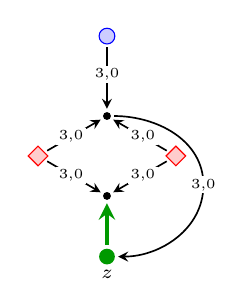
\begin{tikzpicture}[scale=0.35, baseline=-0.5cm]
		\node at (0,-5.1)  [root] (root) {};
		\node at (0,-5.1) [rootlab] {$z$};
		\node at (0,0) [dot] (int) {};
		\node at (0,2.9)  [var_blue] (cent) {};
		\node at (0,-2.9) [dot] (cent1) {};
		\node at (2.5,-1.45)  [var_red_square] (right1) {};
		\node at (-2.5,-1.45)  [var_red_square] (left1) {};
		\draw[testfcn] (cent1) to (root);
		\draw[keps] (left1) to node[labl,pos=0.45] {\tiny 3,0} (int);
		\draw[keps] (right1) to node[labl,pos=0.45] {\tiny 3,0} (int);
		\draw[keps] (cent) to node[labl,pos=0.45] {\tiny 3,0} (int);
		\draw[keps] (right1) to node[labl,pos=0.45] {\tiny 3,0} (cent1);
		\draw[keps] (left1) to node[labl,pos=0.45] {\tiny 3,0} (cent1);
		\draw [keps] (int) to[out=0,in=90] (3.5,-2.5) to [out=-90, in=0] node[labl,pos=0] {\tiny 3,0} (root);
	\end{tikzpicture}\;
	+ \; 2 \;
	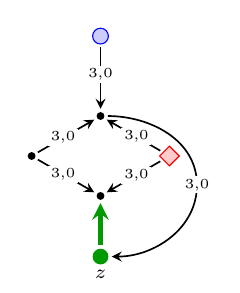
\begin{tikzpicture}[scale=0.35, baseline=-0.5cm]
		\node at (0,-5.1)  [root] (root) {};
		\node at (0,-5.1) [rootlab] {$z$};
		\node at (0,0) [dot] (int) {};
		\node at (0,2.9)  [var_blue] (cent) {};
		\node at (0,-2.9) [dot] (cent1) {};
		\node at (2.5,-1.45)  [var_red_square] (right1) {};
		\node at (-2.5,-1.45)  [dot] (left1) {};
		\draw[testfcn] (cent1) to (root);
		\draw[keps] (left1) to node[labl,pos=0.45] {\tiny 3,0} (int);
		\draw[keps] (right1) to node[labl,pos=0.45] {\tiny 3,0} (int);
		\draw[keps] (cent) to node[labl,pos=0.45] {\tiny 3,0} (int);
		\draw[keps] (right1) to node[labl,pos=0.45] {\tiny 3,0} (cent1);
		\draw[keps] (left1) to node[labl,pos=0.45] {\tiny 3,0} (cent1);
		\draw [keps] (int) to[out=0,in=90] (3.5,-2.5) to [out=-90, in=0] node[labl,pos=0] {\tiny 3,0} (root);
	\end{tikzpicture}\;
	+
	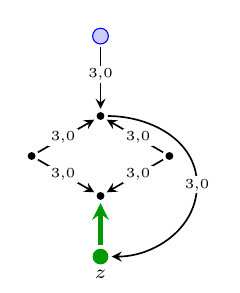
\begin{tikzpicture}[scale=0.35, baseline=-0.5cm]
		\node at (0,-5.1)  [root] (root) {};
		\node at (0,-5.1) [rootlab] {$z$};
		\node at (0,0) [dot] (int) {};
		\node at (0,2.9)  [var_blue] (cent) {};
		\node at (0,-2.9) [dot] (cent1) {};
		\node at (2.5,-1.45)  [dot] (right1) {};
		\node at (-2.5,-1.45)  [dot] (left1) {};
		\draw[testfcn] (cent1) to (root);
		\draw[keps] (left1) to node[labl,pos=0.45] {\tiny 3,0} (int);
		\draw[keps] (right1) to node[labl,pos=0.45] {\tiny 3,0} (int);
		\draw[keps] (cent) to node[labl,pos=0.45] {\tiny 3,0} (int);
		\draw[keps] (right1) to node[labl,pos=0.45] {\tiny 3,0} (cent1);
		\draw[keps] (left1) to node[labl,pos=0.45] {\tiny 3,0} (cent1);
		\draw [keps] (int) to[out=0,in=90] (3.5,-2.5) to [out=-90, in=0] node[labl,pos=0] {\tiny 3,0} (root);
	\end{tikzpicture}\;
\]
and applying Corollary~\ref{cor:convolutions} with $\nu_\ga = -\frac{11}{2}$, each term can be bounded by $\big( \lambda \vee \epsEH \big)^{-\frac{11}{2}} \eps^5 \leq \big( \lambda \vee \epsEH \big)^{-\frac{1}{2}}$. Then the expression in the brackets in \eqref{eq:important_subtree} can instead be written as
\begin{equation} \label{eq:last_tree_decomposition}
	2\;
	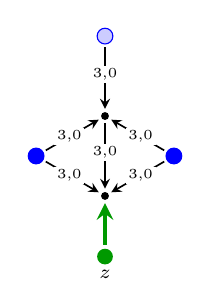
\begin{tikzpicture}[scale=0.35, baseline=-0.5cm]
		\node at (0,-5.1)  [root] (root) {};
		\node at (0,-5.1) [rootlab] {$z$};
		\node at (0,0) [dot] (int) {};
		\node at (0,2.9)  [var_blue] (cent) {};
		\node at (0,-2.9) [dot] (cent1) {};
		\node at (2.5,-1.45)  [var_very_blue] (right1) {};
		\node at (-2.5,-1.45)  [var_very_blue] (left1) {};
		\draw[testfcn] (cent1) to (root);
		\draw[keps] (left1) to node[labl,pos=0.45] {\tiny 3,0} (int);
		\draw[keps] (right1) to node[labl,pos=0.45] {\tiny 3,0} (int);
		\draw[keps] (cent) to node[labl,pos=0.45] {\tiny 3,0} (int);
		\draw[keps] (int) to node[labl,pos=0.45] {\tiny 3,0} (cent1);
		\draw[keps] (right1) to node[labl,pos=0.45] {\tiny 3,0} (cent1);
		\draw[keps] (left1) to node[labl,pos=0.45] {\tiny 3,0} (cent1);
	\end{tikzpicture}
	\; -\; C^\eps_2\;
	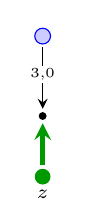
\begin{tikzpicture}[scale=0.35, baseline=-0.7cm]
		\node at (0,-5.1)  [root] (root) {};
		\node at (0,-5.1) [rootlab] {$z$};
		\node at (0,0)  [var_blue] (cent) {};
		\node at (0,-2.9) [dot] (cent1) {};
		\draw[testfcn] (cent1) to (root);
		\draw[keps] (cent) to node[labl,pos=0.45] {\tiny 3,0} (cent1);
	\end{tikzpicture} 
	\;=\;
	2 \;
	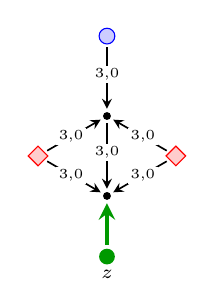
\begin{tikzpicture}[scale=0.35, baseline=-0.5cm]
		\node at (0,-5.1)  [root] (root) {};
		\node at (0,-5.1) [rootlab] {$z$};
		\node at (0,0) [dot] (int) {};
		\node at (0,2.9)  [var_blue] (cent) {};
		\node at (0,-2.9) [dot] (cent1) {};
		\node at (2.5,-1.45)  [var_red_square] (right1) {};
		\node at (-2.5,-1.45)  [var_red_square] (left1) {};
		\draw[testfcn] (cent1) to (root);
		\draw[keps] (left1) to node[labl,pos=0.45] {\tiny 3,0} (int);
		\draw[keps] (right1) to node[labl,pos=0.45] {\tiny 3,0} (int);
		\draw[keps] (cent) to node[labl,pos=0.45] {\tiny 3,0} (int);
		\draw[keps] (int) to node[labl,pos=0.45] {\tiny 3,0} (cent1);
		\draw[keps] (right1) to node[labl,pos=0.45] {\tiny 3,0} (cent1);
		\draw[keps] (left1) to node[labl,pos=0.45] {\tiny 3,0} (cent1);
	\end{tikzpicture}
	+ 4 \;
	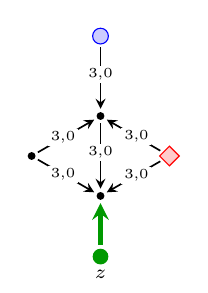
\begin{tikzpicture}[scale=0.35, baseline=-0.5cm]
		\node at (0,-5.1)  [root] (root) {};
		\node at (0,-5.1) [rootlab] {$z$};
		\node at (0,0) [dot] (int) {};
		\node at (0,2.9)  [var_blue] (cent) {};
		\node at (0,-2.9) [dot] (cent1) {};
		\node at (2.5,-1.45)  [var_red_square] (right1) {};
		\node at (-2.5,-1.45)  [dot] (left1) {};
		\draw[testfcn] (cent1) to (root);
		\draw[keps] (left1) to node[labl,pos=0.45] {\tiny 3,0} (int);
		\draw[keps] (right1) to node[labl,pos=0.45] {\tiny 3,0} (int);
		\draw[keps] (cent) to node[labl,pos=0.45] {\tiny 3,0} (int);
		\draw[keps] (int) to node[labl,pos=0.45] {\tiny 3,0} (cent1);
		\draw[keps] (right1) to node[labl,pos=0.45] {\tiny 3,0} (cent1);
		\draw[keps] (left1) to node[labl,pos=0.45] {\tiny 3,0} (cent1);
	\end{tikzpicture}
	\;+\; \left( \; 2 \;
	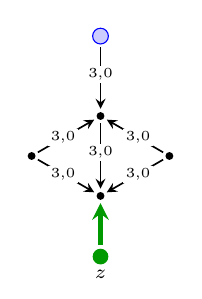
\begin{tikzpicture}[scale=0.35, baseline=-0.5cm]
		\node at (0,-5.1)  [root] (root) {};
		\node at (0,-5.1) [rootlab] {$z$};
		\node at (0,-5.3) {$$};
		\node at (0,0) [dot] (int) {};
		\node at (0,2.9)  [var_blue] (cent) {};
		\node at (0,-2.9) [dot] (cent1) {};
		\node at (2.5,-1.45)  [dot] (right1) {};
		\node at (-2.5,-1.45)  [dot] (left1) {};
		\draw[testfcn] (cent1) to (root);
		\draw[keps] (left1) to node[labl,pos=0.45] {\tiny 3,0} (int);
		\draw[keps] (right1) to node[labl,pos=0.45] {\tiny 3,0} (int);
		\draw[keps] (cent) to node[labl,pos=0.45] {\tiny 3,0} (int);
		\draw[keps] (int) to node[labl,pos=0.45] {\tiny 3,0} (cent1);
		\draw[keps] (right1) to node[labl,pos=0.45] {\tiny 3,0} (cent1);
		\draw[keps] (left1) to node[labl,pos=0.45] {\tiny 3,0} (cent1);
	\end{tikzpicture}
	\; -\; C^\eps_2 \;
	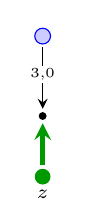
\begin{tikzpicture}[scale=0.35, baseline=-0.7cm]
		\node at (0,-5.1)  [root] (root) {};
		\node at (0,-5.1) [rootlab] {$z$};
		\node at (0,0)  [var_blue] (cent) {};
		\node at (0,-2.9) [dot] (cent1) {};
		\draw[testfcn] (cent1) to (root);
		\draw[keps] (cent) to node[labl,pos=0.45] {\tiny 3,0} (cent1);
	\end{tikzpicture}
	\right),
\end{equation}
The first two diagrams above can again be bounded using Corollary~\ref{cor:convolutions} by a constant multiple of $(\lambda \vee \epsEH)^{- 1/ 2}$.

The last expression in the brackets in \eqref{eq:last_tree_decomposition} needs more attention. Let us define a new kernel 
\[
	\CG_\eps (z_1, z_2) \; := \;
	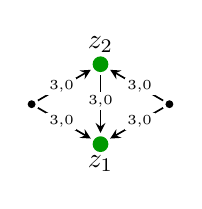
\begin{tikzpicture}[scale=0.35, baseline=-0.55cm]
		\node at (0,0) [root] (int) {};
		\node at (0, 0.7) [] () {$z_2$};
		\node at (0,-2.9) [root] (cent) {};
		\node at (0,-3.6) [] () {$z_1$};
		\node at (2.5,-1.45) [dot] (right1) {};
		\node at (-2.5,-1.45) [dot] (left1) {};
		\draw[keps] (left1) to node[labl,pos=0.45] {\tiny 3,0} (int);
		\draw[keps] (right1) to node[labl,pos=0.45] {\tiny 3,0} (int);
		\draw[keps] (int) to node[labl,pos=0.45] {\tiny 3,0} (cent);
		\draw[keps] (right1) to node[labl,pos=0.45] {\tiny 3,0} (cent);
		\draw[keps] (left1) to node[labl,pos=0.45] {\tiny 3,0} (cent);
	\end{tikzpicture}\;,
\]
which is in fact a function of the difference of the arguments, i.e. $\CG_\eps (z_1, z_2) = \CG_\eps (z_2 - z_1)$. As follows from the order of the singularity of the kernel $K^{\epsEH}$ and \cite[Lemma~7.3]{HM18}, the function $\CG_\eps$ satisfies $|D^k \CG_\eps(z)| \lesssim (\|z\|_\s + \epsEH)^{-5 - |k|_\s}$ for all multiindices $k$ with $|k|_\s$ large enough. Then we conclude from Lemma~\ref{lem:K_bound} that the function $\CG_\eps$ has all the properties listed in Assumption~\ref{a:Kernels} with the values $a_e = 5$ and $r_e = 0$. We denote the kernel $\CG_\eps$ by an edge ``\,\tikz[baseline=-0.1cm] \draw[kernelBig] (0,0) to node[labl,pos=0.45] {\tiny 5,0} (1,0);\,''. Then the first diagram in the brackets in \eqref{eq:last_tree_decomposition} can be represented as
\begin{equation*}
	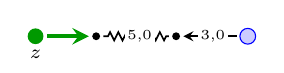
\begin{tikzpicture}[scale=0.35, baseline=0cm]
		\node at (0,0)  [root] (root) {};
		\node at (0,0) [rootlab] {$z$};
		\node at (2.2,0) [dot] (cent1) {};
		\node at (5.1,0) [dot] (int) {};
		\node at (7.7,0)  [var_blue] (cent) {};
		\draw[testfcn] (cent1) to (root);
		\draw[keps] (cent) to node[labl,pos=0.45] {\tiny 3,0} (int);
		\draw[kernelBig] (int) to node[labl,pos=0.45] {\tiny 5,0} (cent1);
	\end{tikzpicture}\;,
\end{equation*}
and one can see that this diagram does not satisfy Assumption~\ref{a:mainContraction}(\ref{it:mainContraction-1}) (recall that $|\s| = 5$). To resolve this problem, we need to use a negative renormalisation (in the sense of Section~\ref{sec:renormalisation}) of the kernel $\CG_\eps$. More precisely, for any smooth function $\eta: \R^4 \times \R^4 \to \R$, we define its negative renormalisation as
\[
	\big( \SR_\eps \CG_\eps \big) (\eta) := \int_{D_\eps} \int_{D_\eps} \CG_\eps(z_1, z_2) \big( \eta(z_1, z_2) - \eta(z_1, z_1) \big) \, \d z_1 \d z_2,
\]
and we graphically depict $\SR_\eps \CG_\eps$ as ``\,\tikz[baseline=-0.1cm] \draw[kernelBig] (0,0) to node[labl,pos=0.45] {\tiny 5,-1} (1,0);\,'', where the label ``$-1$'' refers to the order of renormalisation. Since the renormalisation constant \eqref{e:Phi_C2} can be represented as
\begin{equation*}
 C^\eps_2 = 2 \;
 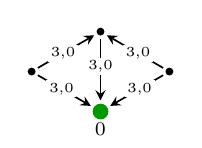
\begin{tikzpicture}[scale=0.35, baseline=-0.55cm]
		\node at (0,0) [dot] (int) {};
		\node at (0,-2.9) [root] (cent) {};
		\node at (0,-2.9) [rootlab] {$0$};
		\node at (2.5,-1.45) [dot] (right1) {};
		\node at (-2.5,-1.45) [dot] (left1) {};
		\draw[keps] (left1) to node[labl,pos=0.45] {\tiny 3,0} (int);
		\draw[keps] (right1) to node[labl,pos=0.45] {\tiny 3,0} (int);
		\draw[keps] (int) to node[labl,pos=0.45] {\tiny 3,0} (cent);
		\draw[keps] (right1) to node[labl,pos=0.45] {\tiny 3,0} (cent);
		\draw[keps] (left1) to node[labl,pos=0.45] {\tiny 3,0} (cent);
	\end{tikzpicture}\;,
\end{equation*}
the expression in the brackets in \eqref{eq:last_tree_decomposition} equals
\begin{equation*}
	2\; 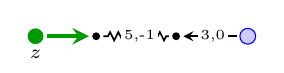
\begin{tikzpicture}[scale=0.35, baseline=-0.1cm]
		\node at (0,0)  [root] (root) {};
		\node at (0,0) [rootlab] {$z$};
		\node at (2.2,0) [dot] (cent1) {};
		\node at (5.1,0) [dot] (int) {};
		\node at (7.7,0)  [var_blue] (cent) {};
		\draw[testfcn] (cent1) to (root);
		\draw[keps] (cent) to node[labl,pos=0.45] {\tiny 3,0} (int);
		\draw[kernelBig] (int) to node[labl,pos=0.45] {\tiny 5,-1} (cent1);
	\end{tikzpicture}\;.
\end{equation*}
This diagram satisfies Assumption~\ref{a:mainContraction}, and using Corollary~\ref{cor:convolutions} we bound its moments by a constant multiple of $(\lambda \vee \epsEH)^{-\bar\kappa}$ for any $\bar\kappa > 0$.

\begin{appendices}

\section{Properties of \cadlag~martingales}
\label{sec:Appendix2}

Following \cite[Ch.~I.4]{JS03}, we list those properties of martingales which are used in the article. Let $(M_t)_{t \geq 0}$ and $(N_t)_{t \geq 0}$ be two \cadlag~square-integrable martingales on the same filtered probability space. Their {\it predictable quadratic covariation} $\langle M, N\rangle_t$ is the unique adapted process with bounded total variation, such that $M_t N_t - \langle M, N\rangle_t$ is a martingale. The {\it quadratic covariation} $[M, N]_t$ is defined by
\begin{equation}%\label{e:Bracket}
	[M, N]_t := M_t N_t - M_0 N_0 - \int_{0}^t M_{s^-} \d N_s - \int_{0}^t N_{s^-} \d M_s\;,
\end{equation}
where $M_{s-} := \lim_{r \uparrow s} M_{r}$ is the left limit of $M$ at time $s$. Another way to define these quadratic covariations is the following: if $0 = t_0 \leq \cdots \leq t_n = t$ is a partition with diameter $\max_i (t_{i+1} - t_{i})$ tending to zero as $n \to \infty$, then $[M, N]_t$ is equal to the limit in probability of the sums $\sum_{i=0}^{n-1} (M_{t_{i+1}} - M_{t_{i}}) (N_{t_{i+1}} - N_{t_{i}})$ as $n \to \infty$ (see \cite[Thm.~I.4.47]{JS03}), and $\langle M, N\rangle_t$ is the probability limit of the sums $\sum_{i=0}^{n-1} \E [(M_{t_{i+1}} - M_{t_{i}}) (N_{t_{i+1}} - N_{t_{i}}) | \Ff_{t_i} ]$, where $(\Ff_t)_{t \geq 0}$ is the underlying filtration \cite[Prop.~I.4.50]{JS03}. The difference of the two bracket processes $[M, N]_t - \langle M, N\rangle_t$ is always a \cadlag~martingale \cite[Prop.~I.4.50]{JS03}. In the case $M = N$, it will be convenient to use the shorthands $[M]_t = [M, M]_t$ and $\langle M \rangle_t = \langle M, M\rangle_t$.

The following is the standard version of the \BDG inequality \cite[6.E.3]{Semimartirgales}.

\begin{proposition}\label{prop:BDGclassic}
	Let $(M_t)_{t \in [0, T]}$ be a \cadlag square integrable martingale. Then, for any $p \geq 1$ there exists a constant $C > 0$, depending on $p$, such that 
	\begin{equation}
		\E \biggl[ \sup_{t \in [0, T]} | M_t |^p \biggr]^{\frac{1}{p}} \leq C \left( \E \left[ [ M]_t^{p / 2} \right] \right)^{\frac{1}{p}}.
	\end{equation}
\end{proposition}

Sometimes it is more convenient to use the \BDG inequality in the following form, which is obtained by approximating $M$ by discrete-time martingales and applying the discrete-time \BDG inequality \cite{HH80}.

\begin{proposition}\label{prop:BDG}
	Let $(M_t)_{t \in [0, T]}$ be a \cadlag square integrable martingale. Then, for any $p \geq 1$ there exists a constant $C > 0$ depending on $p$ such that 
	\begin{equation}\label{eq:BDG}
		\E \biggl[ \sup_{t \in [0, T]} | M_t |^p \biggr]^{\frac{1}{p}} \leq C \biggl( \E \left[ \langle M \rangle_t^{p/2}\right]^{\frac{1}{p}} + \E \biggl[ \sup_{t \in [0, T]} | \Delta_t M |^p \biggr]^{\frac{1}{p}} \biggr),
	\end{equation}
	where $\Delta_t M := M_t - M_{t-}$ is a jump at time $t$.
\end{proposition}

\section{Properties of the function $a^{\ldouble p \rdouble}$}
\label{sec:AppendixStrangePower}
	
	In this appendix we prove some properties of the function $a^{\ldouble p \rdouble}$, defined in \eqref{eq:strange_power}.
	
	\begin{lemma} \label{propertiesExponent}
		For $a, b, p, q > 0$, the following properties hold:
		\begin{enumerate}
			\item $(ab )^{\ldouble p \rdouble} \leq a^{\ldouble p \rdouble} b^{\ldouble p \rdouble}$ and for $p \geq 1$, $(a + b )^{\ldouble p \rdouble} \leq 2^{p-1} (a^{\ldouble p \rdouble} + b^{\ldouble p \rdouble})$;
			\item \emph{monotonicity in the base:} $a^{\ldouble p \rdouble} \leq b^{\ldouble p \rdouble}$ for $p \geq 1$ and $a \leq b$; $a^{\ldouble p \rdouble} \leq b^{\ldouble p \rdouble}$ for $p \leq 1$ and $a \geq b$;
			\item \emph{monotonicity in the exponent:} $a^{\ldouble p \rdouble} \leq a^{\ldouble q \rdouble}$ for $1 \leq p \leq q$; $a^{\ldouble p \rdouble} \leq a^{\ldouble q \rdouble}$ for $q \leq p \leq 1$;
			\item $( a^{\ldouble p \rdouble})^{\ldouble p \rdouble} = a^{\ldouble p^2 \rdouble}$;
			\item if $p \in (0,1]$ and if $\Vert \cdot \Vert$ is any norm with respect to which the function $a \mapsto a^{\ldouble p \rdouble}$ is finite, then $\Vert a^{\ldouble p \rdouble} \Vert \lesssim \Vert a \Vert^{\ldouble p \rdouble}$, where the norm is applied to the functions in $a$; for $p \geq 1$, the opposite inequality holds.
		\end{enumerate}
	\end{lemma}
	
	\begin{proof}
		\begin{enumerate}[leftmargin=*]
			\item By definition $( ab)^{\ldouble p \rdouble} = \max \{ ab, a^p b^p \}$, and $a^{\ldouble p \rdouble} b^{\ldouble p \rdouble} = \max \{ ab, a^p b, a b^p, a^p b^p \}$. Similar computations can be done with summation: $( a + b )^{\ldouble p \rdouble} = \max \{ a + b, (a + b)^p \} \leq 2^{p-1} \max \{ a + b, a^p + b^p \}$ and $a^{\ldouble p \rdouble} + b^{\ldouble p \rdouble} = \max \{ a , a^p \} + \max \{ b, b^p \}$, which implies $a^{\ldouble p \rdouble} + b^{\ldouble p \rdouble} = \max \{ a+b, a^p+b, a+b^p, a^p+b^p \}$.
			\item Let $p \geq 1$. If $a \geq 1$, then $b$ has to be bigger then or equal to $1$ too, and  therefore $b^{\ldouble p\rdouble} = b^p \geq a^p = a^{\ldouble p\rdouble}$. When $a < 1$, we have two cases: $b \geq 1$, which means that $b^{\ldouble p\rdouble} = b^p \geq 1 \geq a = a^{\ldouble p\rdouble}$; or $b < 1$, which implies that $b^{\ldouble p\rdouble} = b \geq a = a^{\ldouble p\rdouble}$. For $p \leq 1$, we can use a similar argument.
			\item When $1 \leq p \leq q$, we have $a^{\ldouble p \rdouble} = a^p \mathbbm{1}_{a \geq 1} + a \mathbbm{1}_{a < 1} \leq a^q \mathbbm{1}_{a \geq 1} + a \mathbbm{1}_{a < 1} = a^{\ldouble q\rdouble}$. When $1 \geq p \geq q$, we have $a^{\ldouble p \rdouble} = a \mathbbm{1}_{a \geq 1} + a^p \mathbbm{1}_{a < 1} \leq a \mathbbm{1}_{a \geq 1} + a^q = a^{\ldouble q\rdouble}$.
			\item We have $( a^{\ldouble p\rdouble})^{\ldouble p\rdouble} = \max \{ \max \{ a, a^p \}, \max \{ a, a^{p} \}^p \}$. This expression equals either $a^{p^2}$ (when $a \geq 1$ and $p \geq 1$ or when $a \leq 1$ and $p \leq 1$) or $a$ (when $a \geq 1$ and $p \leq 1$ or when $a \leq 1$ and $p \geq 1$). Thus, the expression equals $\max \{ a, a^{p^2} \} = a^{\ldouble p^2\rdouble}$.
			\item We have $\Vert a^{\ldouble p\rdouble} \Vert = \Vert a \mathbbm{1}_{a \geq 1} + a^p \mathbbm{1}_{a < 1} \Vert \leq \Vert a \mathbbm{1}_{a \geq 1} \Vert + \Vert a^p \mathbbm{1}_{a < 1} \Vert$. For $p \in (0,1]$, using Jensen's inequality, this expression is bounded by $\Vert a \mathbbm{1}_{a \geq 1} \Vert + \Vert a \mathbbm{1}_{a < 1} \Vert^p \leq 2 \max \{ \Vert a \Vert, \Vert a \Vert^p \} = 2 \Vert a \Vert^{\ldouble p\rdouble}$. The inequality for $p \geq 1$ can be proved analogously. 
			\end{enumerate}
	\end{proof}

\end{appendices}

\bibliographystyle{Martin}
\bibliography{bibliography}

\end{document}
